\documentclass[11pt]{article}
\usepackage[T1]{fontenc}
\usepackage{lmodern}
\usepackage[margin=1.05in]{geometry}
\usepackage{amsmath,amssymb,amsthm,mathtools,mathrsfs}
\usepackage{microtype}
\usepackage{enumitem}
\usepackage{tikz}
\usetikzlibrary{arrows.meta,positioning}
\usepackage{xcolor}
\usepackage[colorlinks=true,linkcolor=blue!45!black,citecolor=blue!45!black,urlcolor=blue!45!black]{hyperref}
\input{glyphtounicode}
\pdfgentounicode=1
\pdftrailerid{}
\hypersetup{pdftitle={Smooth counterexamples to Yau's nodal upper bound in dimensions three and four},pdfsubject={Spectral geometry and nodal sets},pdfauthor={OpenAI}}
\numberwithin{equation}{section}
\newtheorem{theorem}{Theorem}[section]
\newtheorem{proposition}[theorem]{Proposition}
\newtheorem{lemma}[theorem]{Lemma}
\newtheorem{corollary}[theorem]{Corollary}
\theoremstyle{definition}
\newtheorem{definition}[theorem]{Definition}
\theoremstyle{remark}
\newtheorem{remark}[theorem]{Remark}
\newcommand{\R}{\mathbb R}
\newcommand{\C}{\mathbb C}
\newcommand{\N}{\mathbb N}
\newcommand{\Sph}{\mathbb S}
\newcommand{\T}{\mathbb T}
\newcommand{\HH}{\mathcal H}
\newcommand{\cH}{\mathcal H}
\newcommand{\dd}{\,\mathrm d}
\DeclareMathOperator{\vol}{vol}
\DeclareMathOperator{\supp}{supp}
\DeclareMathOperator{\tr}{tr}
\DeclareMathOperator{\Id}{Id}
\DeclareMathOperator{\diag}{diag}
\DeclareMathOperator{\Div}{div}
\DeclareMathOperator{\divg}{div}
\DeclareMathOperator{\Hess}{Hess}
\DeclareMathOperator{\grad}{grad}
\DeclareMathOperator{\dist}{dist}
\setlist{itemsep=2pt,topsep=4pt}
\setlength{\emergencystretch}{2em}
\title{Smooth counterexamples to Yau's nodal upper bound\\in dimensions three and four}
\author{OpenAI}
\date{September 23, 2026}
\begin{document}
\maketitle
\begin{abstract}
We construct a smooth metric on the three-sphere, arbitrarily close to the round metric in the smooth topology, and a smooth metric on $S^2\times\T^2$ for which sequences of exact real Laplace eigenfunctions have unbounded nodal measure divided by the square root of the eigenvalue. Each sequence belongs to one fixed metric. Thus the upper-bound part of Yau's nodal conjecture fails for smooth metrics in dimensions three and four.
\end{abstract}
\section{Introduction}
\label{sec:introduction}

Let $(M,g)$ be a closed connected smooth Riemannian manifold of dimension $d$.
We write $-\Delta_g u=\lambda u$ for a nonzero real Laplace eigenfunction
with $\lambda>0$, and $Z_u=\{x\in M:u(x)=0\}$ for its nodal set. Yau's
nodal conjecture in the smooth category predicts constants $c_g,C_g>0$,
depending on this one metric, such that
\begin{equation}\label{eq:intro-yau}
 c_g\sqrt\lambda\le\mathcal H_g^{d-1}(Z_u)
              \le C_g\sqrt\lambda
\end{equation}
for every such eigenfunction. The distinction between a fixed metric and a
metric chosen anew at each eigenvalue is essential. The lower and upper
inequalities are also logically separate. This paper disproves the upper
inequality in two low-dimensional smooth settings.

\begin{theorem}\label{thm:main}
Let $g_*$ be the round metric on $\Sph^3$. Every neighborhood of $g_*$ in
the $C^\infty$ topology contains a smooth Riemannian metric $g_\infty$ for
which there are nonzero smooth real functions $u_j$ and positive numbers
$\lambda_j$ satisfying
\[
 -\Delta_{g_\infty}u_j=\lambda_j u_j,\qquad
 \lambda_j\longrightarrow\infty,\qquad
 \frac{\HH^2_{g_\infty}(Z_{u_j})}{\sqrt{\lambda_j}}
       \longrightarrow\infty.
\]
\end{theorem}

\begin{theorem}\label{thm:four}
There are a smooth Riemannian metric $g_\infty$ on $S^2\times\T^2$,
nonzero smooth real functions $u_j$, and positive numbers
$\lambda_j\to\infty$ such that
\[
 -\Delta_{g_\infty}u_j=\lambda_j u_j,\qquad
 \frac{\cH^3_{g_\infty}(Z_{u_j})}{\sqrt{\lambda_j}}
       \longrightarrow\infty.
\]
\end{theorem}

Theorem~\ref{thm:main} gives a negative resolution of the upper-bound
part of the smooth nodal conjecture already in dimension three, with
metrics arbitrarily close to the round sphere. Theorem~\ref{thm:four}
provides a distinct four-dimensional topology and metric realization.
Neither theorem asserts a power-law excess, and neither contradicts the
lower-bound part of \eqref{eq:intro-yau}.
In dimensions at least five, a separate companion constructs fixed-metric
counterexamples with a fixed positive power-law excess
\cite[Theorem~1.1 and Corollary~5.6]{OpenAINodalPower2026}.

\paragraph{Context.}
Yau formulated the nodal measure problem for Laplace eigenfunctions on
closed manifolds \cite{Yau1982}. Donnelly and Fefferman established both
sharp estimates for real-analytic metrics
\cite[Theorem~1.2]{DonnellyFefferman1988}.
For smooth metrics, Hardt and Simon obtained a general non-polynomial
upper estimate \cite[Section~5]{HardtSimon1989}. Logunov later proved
a polynomial upper estimate in dimensions at least three
\cite{LogunovUpper2018}, as well as the sharp lower estimate
\cite[Theorem~1.1]{LogunovLower2018}. The gap between polynomial growth
and the conjectured square-root upper bound is where the examples here lie.

The smooth surface case has a separate quantitative history.
Br\"uning proved the sharp square-root lower estimate
\cite[Satz~2]{Bruning1978}. Donnelly and Fefferman obtained the upper
estimate $C_g\lambda^{3/4}$ \cite{DonnellyFefferman1990}, and Logunov
and Malinnikova improved its exponent to $3/4-\beta$ for a universal
$\beta\in(0,1/4)$ \cite{LogunovMalinnikova2018}.
Under intermediate regularity hypotheses, Hezari proved bounds for
Gevrey metrics and a specified quasianalytic class
\cite[preprint version, Theorems~1.1 and~1.2]{Hezari2023}; these are not statements for
arbitrary smooth metrics.

Metric flexibility has also been used to prescribe nodal geometry.
On a closed manifold of dimension at least three, Enciso and Peralta-Salas
realized any smooth connected closed orientable separating hypersurface
as the nodal set of a first nonconstant eigenfunction by choosing the metric
\cite[preprint version, Theorem~1.1]{EncisoPeraltaSalas2015}.
Their work with Steinerberger prescribes any smooth connected closed
separating hypersurface in the same dimensions, within each conformal class
and with fixed total volume, up to an ambient diffeomorphism arbitrarily
close to the identity in $C^0$
\cite[preprint version, Theorem~1.1]{EncisoPeraltaSalasSteinerberger2017}.
On a fixed round sphere or flat torus, high-energy eigenfunctions can
have nodal components of prescribed complicated topology
\cite{EncisoPeraltaSalasTorres2018}. Krauz has prescribed individual
nodal configurations on the sphere by metric choice \cite{Krauz2025}.
These results address nodal topology, including at high frequencies on
fixed analytic metrics. The distinction in Theorems~\ref{thm:main}
and~\ref{thm:four} is the unbounded normalized nodal measure along a
sequence of eigenfunctions for one fixed smooth metric.

\paragraph{Two constructions and their common logic.}
Each branch starts from a background metric with explicit high-frequency
eigenfunctions and a region left unchanged by all local corrections.
A smooth logarithmic envelope is corrugated in transverse directions so
that its integrated gradient becomes arbitrarily large without losing
the strict Hessian inequality needed for localized complex waves.
Finite phase and transport jets give quasimodes with arbitrarily small
weighted residual. This construction is related to complex-phase WKB
quasimodes \cite[Section~3]{DenckerSjostrandZworski2004}; the weighted
finite-order estimates required here are proved in the wave sections. A Gaussian superposition makes the real value and
first derivative jointly nonvanishing and supplies many strict
opposite-sign tests along short coordinate segments. These tests form a
lower semicontinuous score bounded by the nodal Hausdorff measure, even
when the zero set is not assumed regular. Random-wave studies of typical
nodal volume provide a related probabilistic backdrop
\cite{RudnickWigman2007,Wigman2008}; the argument here selects one wave
with a large stable sign score and proves its realization under a metric
change, rather than importing a random-wave nodal-volume formula.

The obstacle is to replace each quasimode by an exact eigenfunction of an
\emph{ordinary} Laplace--Beltrami operator while retaining every sign.
In the three-sphere branch, a scalar conductivity and independent density
first correct the equation. Division by a positive solution of a
semilinear elliptic equation makes them satisfy the three-dimensional
metric determinant identity in the active region; a transverse tensor
change repairs the remaining defect in a clean annulus. In the
$S^2\times\T^2$ branch, a conformal scalar correction has coercive
linearization $\Delta_h-2\lambda$, and a change tangent to the level
sets enforces the four-dimensional determinant identity. These are
separate exactification arguments, not a dimension-independent
realization lemma.

Figure~\ref{fig:two-repairs} isolates the two dimension-specific repairs.
The first converts a scalar conductivity and density into a metric; the
second uses a conformal correction before repairing a rank-three tangent
bundle. In both rows, the last tensor change annihilates the gradient of
the chosen eigenfunction and therefore leaves its corrected equation
unchanged.
\begin{figure}[htbp]
\centering
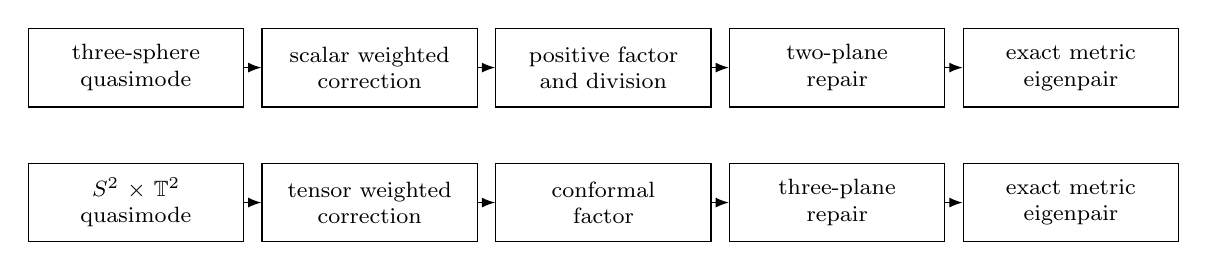
\begin{tikzpicture}[
  every node/.style={draw,align=center,font=\footnotesize,minimum height=10mm,text width=25mm},
  >=Latex,node distance=2.2mm]
  \node (a) {three-sphere\\quasimode};
  \node[right=of a] (b) {scalar weighted\\correction};
  \node[right=of b] (c) {positive factor\\and division};
  \node[right=of c] (d) {two-plane\\repair};
  \node[right=of d] (e) {exact metric\\eigenpair};
  \node[below=7mm of a] (f) {$S^2\times\T^2$\\quasimode};
  \node[right=of f] (g) {tensor weighted\\correction};
  \node[right=of g] (h) {conformal\\factor};
  \node[right=of h] (i) {three-plane\\repair};
  \node[right=of i] (j) {exact metric\\eigenpair};
  \foreach \x/\y in {a/b,b/c,c/d,d/e,f/g,g/h,h/i,i/j}
    \draw[->] (\x) -- (\y);
\end{tikzpicture}
\caption{Two routes from localized quasimodes to exact eigenfunctions of
ordinary metrics. The repairs preserve the strict sign tests used later
to pass to one fixed limiting metric.}
\label{fig:two-repairs}
\end{figure}

Finally, a perturbation preserving the selected eigenfunction makes its
eigenvalue simple. A strict lower bound for the sign score then persists for all metrics
in a neighborhood. Nested metric neighborhoods retain each previous
witness while inserting the next one, and converge to the single smooth
metric required by each theorem. The large-frequency thresholds may
depend on each fixed envelope; no uniform spectral gap is required.
Uhlenbeck's generic simplicity theorem \cite{Uhlenbeck1976} is context
for this spectral step, not a substitute for the selected-mode-preserving
perturbations proved here.

Taking the product of the three-sphere metric with any fixed closed
Riemannian manifold and pulling back its eigenfunctions gives further
qualitative failures in higher dimensions. This elementary extension
does not assert a power-law excess in dimensions three or four.

Together with the surface theorem \cite[Theorem~1.1]{OpenAINodalSurfaces2026},
Theorem~\ref{thm:main} and this product observation give the exact universal
dimension threshold: among dimensions $d\ge2$, the upper inequality in
\eqref{eq:intro-yau}, with a metric-dependent constant uniform over all
nonzero real eigenfunctions of positive eigenvalue, holds for every closed
connected smooth Riemannian manifold precisely when $d=2$. For each
$d\ge3$, there is one fixed smooth metric with a violating sequence.

\paragraph{Organization and conventions.}
The three-sphere proof first constructs amplifiable profiles in
Section~\ref{sec:profiles}, waves and signs in Section~\ref{sec:waves},
an exact ordinary metric in Section~\ref{sec:exactification}, and a
fixed-metric limit in Sections~\ref{sec:pinning}--\ref{sec:persistence}.
The $S^2\times\T^2$ proof then develops its own envelopes in
Section~\ref{sec:envelopes}, waves in Section~\ref{sec:four-waves},
sign score in Section~\ref{sec:signs}, metric correction in
Section~\ref{sec:correction}, and spectral limit in
Section~\ref{sec:spectral}. Throughout, gradients and divergences
carry the displayed metric unless stated otherwise. Hausdorff measure
is taken for the Riemannian distance, with a fixed standard
normalization. All finite derivative and residual orders are chosen
before sending the frequency to infinity.

\part*{The three-sphere construction}
\section{Profiles with large mean gradient}
\label{sec:profiles}

A smooth real function $\phi$ will determine the amplitude envelope
$e^{n\phi}$ at frequency $n$ for the waves in Section~\ref{sec:waves}.
Their construction
requires a strict Hessian inequality, whereas their eventual nodal-area
lower bound grows with the integrated gradient of $\phi$.  We show that
these two requirements are compatible: a local perturbation can increase
the gradient integral arbitrarily while preserving the Hessian condition
and changing $\phi$ arbitrarily little in $C^0$.  We then apply this
construction on $\Sph^3$, preserving a prescribed radial profile
outside one coordinate cube.

Throughout this section, gradients, Hessians, and norms are computed using a
fixed smooth Riemannian metric $g$ on a three-dimensional manifold.  Write
\[
 a_\phi=\grad_g\phi,\qquad
 L_\phi=(1+|a_\phi|^2)^{1/2},\qquad H_\phi=\Hess_g\phi.
\]

\begin{definition}[Strict and full profiles]
\label{def:strict-profile}
A smooth function $\phi$ is \emph{strict} at a point if there exists a real
vector $b$ at that point such that
\begin{equation}
 b\perp a_\phi,\qquad |b|=L_\phi,\qquad
 H_\phi(a_\phi,a_\phi)+H_\phi(b,b)>0.
 \label{eq:profile-strict}
\end{equation}
It is \emph{full} at that point if the last inequality holds for every $b$
satisfying the first two conditions.
\end{definition}

For a symmetric form $H$ and a unit vector $v\perp a$, it is convenient to set
\[
 \mathcal T(H,a;v)=H(a,a)+(1+|a|^2)H(v,v).
\]
Fullness on a compact set where $a_\phi$ does not vanish gives a positive
minimum of $\mathcal T(H_\phi,a_\phi;v)$ over the transverse unit-circle
bundle.  That minimum is allowed to depend on the profile.

The main construction in this section is local.

\begin{proposition}[Amplification of the mean gradient]
\label{prop:profile-amplification}
Let $\Omega$ be a coordinate cube with compact closure in a smooth
three-dimensional Riemannian manifold.  Suppose that $\phi$ is smooth on a
neighborhood of $\overline\Omega$, is strict there, and satisfies
$a_\phi\ne0$ there.  Given $T>0$ and $\varepsilon>0$, there is a smooth
function $\widehat\phi$ on the same neighborhood such that
\[
 \supp(\widehat\phi-\phi)\Subset\Omega,\qquad
 \|\widehat\phi-\phi\|_{C^0(\Omega)}<\varepsilon,
 \qquad
 \int_\Omega |a_{\widehat\phi}|\,\dd V_g>T.
\]
The function $\widehat\phi$ is strict and has nonvanishing gradient on
$\overline\Omega$.

More precisely, there is a constant $\eta>0$, determined only by the fixed
periodic functions chosen below, such that one finite cycle of the
construction multiplies
$\int_\Omega|a_\phi|\,\dd V_g$ by at least $1+\eta$.  The cycle can have
arbitrarily small $C^0$ size.  Its patch sizes and frequency thresholds may
depend on the entire incoming profile and metric.
\end{proposition}

The cycle has two parts.  A first perturbation makes the profile full on a
fixed positive fraction of its gradient mass while changing the gradient
arbitrarily little.  A radial perturbation in the two transverse variables
then increases the gradient on a fixed fraction of that region.  The radial
perturbation preserves strictness, allowing the cycle to be repeated.

\subsection{Localization and periodic averaging}

We use two elementary facts in both parts of the construction.

\begin{lemma}[Disjoint patches and averaging]
\label{lem:profile-localization}
Let $U$ be an open subset of a relatively compact coordinate cube, and let
$\mu$ be a finite measure given by a positive smooth density.
\begin{enumerate}
 \item Given an open neighborhood of each point of $U$, one can choose
 finitely many coordinate cubes $P_j$, with disjoint interiors and closures
 contained in those neighborhoods and in $U$, and functions
 $0\le\chi_j\le1$ in $C_c^\infty(P_j)$, such that $\chi_j=1$ on open
 cores $C_j\Subset P_j$ and
 \[
   \mu\Bigl(\bigcup_j C_j\Bigr)\ge\frac12\mu(U).
 \]
 In particular, the supports of the $\chi_j$ are pairwise disjoint.
 \item Suppose that $y$ is a smooth submersion to $\R^q$, with $q=1$ or
 $2$, on a neighborhood of $\overline P$, and that $C\Subset P$ is
 measurable.  Let $E\subset\R^q$ be periodic with respect to a full
 lattice, have boundary of measure zero in a period cell, and occupy a
 fraction $p$ of that cell.  Then
 \[
  \lim_{N\to\infty}
  \mu\{x\in C:Ny(x)\in E\}=p\,\mu(C).
 \]
\end{enumerate}
\end{lemma}

\begin{proof}
For the first assertion, choose a compact subset of $U$ carrying more than
three quarters of its mass.  A finite subcover of the prescribed
neighborhoods has a Lebesgue number on this compact set.  A sufficiently fine
coordinate grid therefore gives finitely many cubes, each with closure in
one of the prescribed neighborhoods and in $U$, whose union contains that
compact set except for grid faces.  The faces have zero mass.  Shrinking the
cores inside these cubes loses arbitrarily little mass, and smooth cutoffs
supported in the cubes can be chosen to equal one on the cores.

For the second assertion, submersion coordinates and a finite partition of
unity express the pushforward of $\mu|_C$ under $y$ as an integrable density
on $\R^q$.  Thus it suffices to average the bounded periodic function
$\mathbf 1_E(N\cdot)$ against an $L^1$ function.  For the indicator of a
rectangle, the assertion follows by tiling with period cells and estimating
the cells meeting the rectangle's boundary.  Approximation of an $L^1$
function by finite linear combinations of rectangle indicators proves the
claim.  The boundary assumption on $E$ ensures that its cell average is
well defined and unchanged by choices on its boundary.
\end{proof}

We fix a smooth function $h$ of period one such that
\[
 h''(t)=2\cos(2\pi t).
\]
For example, $h(t)=-(2\pi^2)^{-1}\cos(2\pi t)$.  The periodic set
\[
 E_h=\{t:h''(t)>1\}
\]
has fraction $p_h=1/3$ in each period.

\subsection{Preparing a full region}

\begin{lemma}[Preparation]
\label{lem:profile-preparation}
Under the hypotheses of Proposition~\ref{prop:profile-amplification}, let
$0<\epsilon_p\le1/3$ and $\varepsilon>0$.  There is a smooth strict
function $\psi$, with nonvanishing gradient on $\overline\Omega$, such that
\[
 \supp(\psi-\phi)\Subset\Omega,\qquad
 \|\psi-\phi\|_{C^0(\Omega)}<\varepsilon,
 \qquad |a_\psi-a_\phi|\le\epsilon_p|a_\phi|
 \quad\hbox{on }\overline\Omega.
\]
Its full region $U\subset\Omega$ satisfies
\begin{equation}
 \int_U|a_\psi|\,\dd V_g
 \ge\frac{p_h}{8}\int_\Omega|a_\psi|\,\dd V_g.
 \label{eq:prepared-mass}
\end{equation}
The change $\psi-\phi$ can, in addition, be made arbitrarily small in
$C^1$.
\end{lemma}

\begin{proof}
Put $a=a_\phi$.  At each point, choose a strict unit direction $v\perp a$.
Because $a$ does not vanish, the flow-box construction gives a local first
integral $s$, with $\dd s(a)=0$, whose differential at the point is any
prescribed nonzero covector annihilating $a$.  Prescribe it also to
annihilate $v$.  On a sufficiently small neighborhood, the line
\[
 a^\perp\cap\ker\dd s
\]
continues to be strict, with a positive margin on a smaller compact
neighborhood.  The differential $\dd s$ remains nonzero there.

Apply Lemma~\ref{lem:profile-localization} to these neighborhoods with
$\dd\mu=|a|\,\dd V_g$.  It gives finitely many cubes and cutoff-one cores
capturing at least half the mass.  We first describe the perturbation on
one cube, suppressing its index.  Let $\chi$ be its cutoff.  For a constant
$C>0$ to be fixed before $N$, set
\[
 \psi_N=\phi+C N^{-2}\chi h(Ns).
\]
Direct differentiation gives, uniformly on the patch,
\begin{align*}
 a_{\psi_N}
 &=a+\frac C N\chi h'(Ns)\grad s
       +\frac C{N^2}h(Ns)\grad\chi,\\
 H_{\psi_N}
 &=H_\phi+C\chi h''(Ns)\,\dd s\otimes\dd s+O(N^{-1}).
\end{align*}
All constants in this proof may depend on the fixed patch data, including
$C$, but not on $N$.

For large $N$, choose a unit vector $v_N$ on the line
\[
 a_{\psi_N}^{\perp}\cap\ker\dd s.
\]
This line tends uniformly to the old strict line.  The added leading
Hessian has zero value on $v_N$, while
$\dd s(a_{\psi_N})=O(N^{-1})$.  Its value on the new gradient is
therefore $O(N^{-2})$, even on the portions where $h''$ is negative.  The
remaining Hessian error is $O(N^{-1})$.  The old strict margin consequently
preserves strictness for all sufficiently large $N$.

We choose $C$ to obtain fullness on the cutoff-one core where $Ns\in E_h$.
For the old gradient, consider the symmetric form on $a^\perp$
\[
 B=(1+|a|^2)H_\phi|_{a^\perp}+H_\phi(a,a)\Id.
\]
In an orthonormal basis $(v,w)$ with $\dd s(v)=0$ and
$w=\grad s/|\dd s|$, its $vv$ entry is bounded below by some $m>0$.
All its entries are bounded on the patch.  Adding
\[
 C(1+|a|^2)|\dd s|^2\,w\otimes w
\]
makes $B$ uniformly positive definite when $C$ is sufficiently large.
Indeed, if $|B_{vw}|\le M$ and $B_{ww}\ge-M$, it is enough to make the
new $ww$ entry exceed $M^2/m+m$; the Schur complement is then positive.
The factor $(1+|a|^2)|\dd s|^2$ has a positive patch minimum, so a finite
$C$ suffices.  On the specified core $\chi=1$ and $h''>1$, so the actual
leading addition is at least this large.  Changing the gradient by
$O(N^{-1})$ and adding the Hessian remainder preserves its positive
minimum for large $N$.  Thus $\psi_N$ is full there.

Perform these perturbations on the finite disjoint patches, with their
chosen constants $C$, using a common sufficiently large $N$.  The changes
are arbitrarily small in $C^1$, preserve nonvanishing, and have compact
support in $\Omega$.  Lemma~\ref{lem:profile-localization} shows that the
union $G_N$ of the cutoff-one regions with $Ns\in E_h$ satisfies
\[
 \int_{G_N}|a|\,\dd V_g
 \ge\frac{p_h}{4}\int_\Omega|a|\,\dd V_g
\]
for sufficiently large $N$.  Choose $N$ still larger so that the stated
pointwise relative gradient bound holds.  With
$\mathcal M(\zeta)=\int_\Omega|a_\zeta|\,\dd V_g$, the full region
therefore has mass at least
\[
 (1-\epsilon_p)\frac{p_h}{4}\mathcal M(\phi)
 \ge\frac{p_h(1-\epsilon_p)}{4(1+\epsilon_p)}\mathcal M(\psi_N)
 \ge\frac{p_h}{8}\mathcal M(\psi_N).
\]
Fullness is open where the gradient is nonzero, so this gives the asserted
open full region.  The $C^0$ bound and any additional prescribed $C^1$
smallness follow by increasing $N$ once more.
\end{proof}

\subsection{Radial corrugation in two transverse variables}

Fix numbers
\[
 0<r_0<r_1<r_2<R<\frac14
\]
and a smooth nonnegative function $f'$ supported in $(r_0,R)$, with
$f'\ge c_1>0$ on $(r_1,r_2)$.  Define
$f(s)=\int_0^s f'(t)\,\dd t$.  On every disk of radius $R$ centered at
a point of $\mathbb Z^2$, define $F$ by the radial function $f$; extend it
by the constant $f(R)$ off these disks.  The result is a smooth
$\mathbb Z^2$-periodic function, constant near the disk centers and
boundaries.  Its annular set
\[
 E_F=\bigcup_{k\in\mathbb Z^2}
       \{y:r_1<|y-k|<r_2\}
\]
has a fixed positive fraction $p_F=\pi(r_2^2-r_1^2)$ in a period cell.

\begin{lemma}[Transverse radial corrugation]
\label{lem:radial-corrugation}
There are constants $\delta>0$ and $g_0>0$, depending only on the fixed
function $F$, with the following property.  Let $\psi$ be full with
nonvanishing gradient on a neighborhood of the closure of a relatively
compact coordinate patch $P$.  Suppose that
$y=(y_1,y_2)$ is a smooth submersion there, with
\[
 \dd y(a_\psi)=0,
 \qquad\text{both nonzero singular values of }\dd y
       \text{ in }[1/2,2].
\]
Let $A>0$ be constant and satisfy $1/2\le A/|a_\psi|\le2$, and let
$0\le\chi\le1$ belong to $C_c^\infty(P)$.  Set
\[
 \Phi_N=\psi+\frac{\delta A}{N}\chi F(Ny).
\]
For every sufficiently large integer $N$, the function $\Phi_N$ is strict
and has nonvanishing gradient on $\overline P$.  Moreover,
$\|\Phi_N-\psi\|_{C^0(P)}\to0$.  Given any $\epsilon_r>0$, all
sufficiently large $N$ satisfy
\begin{align}
 |a_{\Phi_N}|&\ge(1-\epsilon_r)|a_\psi|
                      &&\text{on }\overline P,\label{eq:radial-no-loss}\\
 |a_{\Phi_N}|&\ge(1+g_0-\epsilon_r)|a_\psi|
                      &&\text{where }\chi=1\text{ and }Ny\in E_F.
                      \label{eq:radial-gain}
\end{align}
The frequency thresholds may depend on all the fixed patch data and on
$\epsilon_r$; the constants $\delta,g_0$ do not.
\end{lemma}

\begin{proof}
Put $a=a_\psi$ and $a_N=a_{\Phi_N}$.  When $Ny$ lies in a periodic disk,
let $d_R,d_T$ be the radial and angular unit-coefficient combinations of
$\dd y_1,\dd y_2$.  The singular-value hypothesis gives
\[
 \frac12\le |d_R|,|d_T|\le2.
\]
These covectors need not be orthogonal in the metric.  Outside the disks,
set the leading derivatives $f',f'',f'/s$ to zero.  There, or in the
constant central portions of the disks, choose any orthonormal coefficient
pair when such notation is needed.  Set $f'/s=0$ at the center.  Since $f$
is constant near the center, this agrees with its smooth continuation.

The exact gradient formula and the Hessian expansion are
\begin{equation}
 \begin{aligned}
 a_N&=a+q\,d_R^\sharp+e_N,\\
 q&=\delta A\chi f',\qquad
 e_N=\frac{\delta A}{N}F(Ny)\grad\chi,
 \end{aligned}
 \label{eq:radial-gradient}
\end{equation}
\begin{equation}
 H_{\Phi_N}
 =H_\psi+N\delta A\chi
       \left[f''d_R^2+\frac{f'}s d_T^2\right]+E_N,
 \label{eq:radial-hessian}
\end{equation}
with
\begin{equation}
 |E_N|\le C_P\left((\chi+|\dd\chi|)f'+N^{-1}\right).
 \label{eq:radial-remainder}
\end{equation}
Here and below $C_P$ denotes a finite constant depending on the fixed
patch data, independent of $N$.  To check the remainder, its terms are
\begin{align*}
 &\delta A\chi\sum_i F_i(Ny)\Hess y_i,\\
 &\delta A\left(\dd\chi\otimes\sum_i F_i(Ny)\dd y_i
       +\sum_i F_i(Ny)\dd y_i\otimes\dd\chi\right),\\
 &\frac{\delta A}{N}F(Ny)\Hess\chi.
\end{align*}
Since $|(F_1,F_2)|=f'$, these give
Equation~\eqref{eq:radial-remainder}.  In the constant portions of $F$,
its value contributes only to $e_N$ and to the last displayed term.

We first control the leading Hessian trace in
\eqref{eq:radial-hessian}.  The leading increment in
\eqref{eq:radial-gradient} is perpendicular to $a$, so
\[
 |a_N|\ge |a|-|e_N|.
\]
Thus $a_N$ is nonzero for large $N$.  Choose a vector $b_N$ satisfying
\[
 b_N\perp a_N,\qquad d_R(b_N)=0,\qquad
 |b_N|=L_N:=(1+|a_N|^2)^{1/2}.
\]
The two linear constraints have a nonzero common solution in dimension
three.  They imply
\[
 \langle a,b_N\rangle=-\langle e_N,b_N\rangle.
\]
Because $|a|$ has a positive patch minimum, the component of $b_N/L_N$
along $a$ tends uniformly to zero.  The kernel of $\dd y$ is precisely
the line spanned by $a$.  Its singular-value lower bound and the identity
$d_R(b_N)=0$ consequently give, for all sufficiently large $N$,
\[
 |d_T(b_N)|=|\dd y(b_N)|\ge\frac14 L_N.
\]
Also $A\le3L_N$ for large $N$, and
\[
 |d_R(a_N)|\le4\delta A\chi f'+2|e_N|.
\]
With $K=\|f''\|_\infty$ and
$B_N=f''d_R^2+(f'/s)d_T^2$, it follows that
\begin{align*}
 B_N(a_N,a_N)+B_N(b_N,b_N)
 &\ge\frac1{16}L_N^2\frac{f'}s-K|d_R(a_N)|^2\\
 &\ge\frac1{16}L_N^2\frac{f'}s
       -288K\delta^2L_N^2(f')^2-8K|e_N|^2.
\end{align*}
The estimate uses $(x+y)^2\le2x^2+2y^2$; in particular, its final error is
$O_P(N^{-2})$.  Write $S_0=\sup_s sf'(s)>0$.  Choose once and for all
\[
 0<\delta^2\le\frac1{9216KS_0}.
\]
Then $(f')^2\le S_0 f'/s$ gives
\begin{equation}
 \begin{split}
 N\delta A\chi
   \bigl[B_N(a_N,a_N)+B_N(b_N,b_N)\bigr]
 \ge N\delta A\chi\frac{L_N^2}{32}\frac{f'}s
       -C_P N^{-1}.
 \end{split}
 \label{eq:radial-leading-trace}
\end{equation}
All constants used to choose $\delta$ depend only on $F$ and the
numerical singular-value bounds.

We next control the transition where the favorable leading term can be
small.  A nonnegative smooth cutoff satisfies
\[
 |\dd\chi|\le C_P\sqrt\chi.
\]
Indeed, extend it by zero in the coordinate chart.  If its Euclidean
Hessian is bounded by $M>0$, the Taylor inequality at
$x-M^{-1}D\chi(x)$ gives
$|D\chi(x)|^2\le2M\chi(x)$; metric equivalence gives the stated bound.
Consequently, with $t=\chi f'$, Equations~\eqref{eq:radial-gradient}
and~\eqref{eq:radial-remainder} imply
\begin{equation}
 |a_N-a|\le C_P(t+N^{-1}),\qquad
 |E_N|\le C_P(t+\sqrt t+N^{-1}).
 \label{eq:radial-small-product}
\end{equation}

Let $m>0$ be the minimum of the full trace
$\mathcal T(H_\psi,a;v)$ over the transverse unit circles on
$\overline P$.  Project $b_N/L_N$ onto $a^\perp$ and normalize; for
large $N$ this gives a unit vector $v_N\perp a$ differing from
$b_N/L_N$ by $O_P(N^{-1})$.  Using also
$|L_N-L_\psi|\le|a_N-a|$, the base Hessian trace is at least
\[
 H_\psi(a_N,a_N)+H_\psi(b_N,b_N)
 \ge m-C_P(t+N^{-1}).
\]
The vectors $a_N,b_N$ are uniformly bounded for this fixed patch, so the
trace of the remainder in \eqref{eq:radial-small-product} is
bounded in absolute value by $C_P(t+\sqrt t+N^{-1})$.
Choose $t_0>0$ sufficiently small that these terms involving $t$ and
$\sqrt t$ total less than $m/4$ when $t\le t_0$.  For sufficiently large
$N$, Equation~\eqref{eq:radial-leading-trace} now gives a strictly
positive total trace throughout $t\le t_0$.

On the complementary region $t\ge t_0$, one has $s\le R$, and the
positive term in \eqref{eq:radial-leading-trace} is at least
\[
 \frac{N\delta A t_0}{32R}.
\]
It tends to infinity and dominates the bounded base and remainder traces.
This proves strictness for all sufficiently large $N$.  In this argument
$t_0$ and the frequency threshold can depend on the full margin $m$ and
all patch derivatives.  The choice of $\delta$ is already fixed.  In
particular, the region $t\to0$ requires no lower bound for the product
$Nt$.

Finally, exact orthogonality in the leading gradient gives
\[
 |a+q d_R^\sharp|^2=|a|^2+q^2|d_R|^2.
\]
The uniform error $e_N=O_P(N^{-1})$ proves
\eqref{eq:radial-no-loss}.  Where $\chi=1$ and $Ny\in E_F$,
the bounds $A\ge|a|/2$ and $|d_R|\ge1/2$ give
\[
 |a+q d_R^\sharp|
 \ge |a|\sqrt{1+\frac{\delta^2c_1^2}{16}}.
\]
Set
\[
 g_0=\sqrt{1+\frac{\delta^2c_1^2}{16}}-1>0.
\]
Decreasing the fixed $\delta$ if necessary, assume $g_0\le1$.  The
positive minimum of $|a|$ allows $|e_N|\le\epsilon_r|a|$ for large
$N$, proving \eqref{eq:radial-gain}.  The $C^0$ convergence
follows directly from the factor $N^{-1}$ in the definition of $\Phi_N$.
\end{proof}

\subsection{A fixed gain and finite iteration}

\begin{proof}[Proof of Proposition~\ref{prop:profile-amplification}]
Keep the periodic functions and the constants from
Lemma~\ref{lem:radial-corrugation} fixed.  Define
\[
 \theta=\frac{p_h p_F}{64},\qquad
 t_* =\theta g_0,\qquad \eta=\frac{t_*}{4}>0.
\]
We prove the cycle statement, allowing any prescribed positive $C^0$
budget for that cycle.

Apply Lemma~\ref{lem:profile-preparation} with
$\epsilon_p\le\min(1/3,t_*/16)$ and half the $C^0$ budget.  Write
$\psi$ for the resulting profile and $U$ for its full region.  The
preparation, including its frequency, is now held fixed.  On a sufficiently
small neighborhood of each point of $U$, the flow-box construction gives
two first integrals $y_1,y_2$ of $a_\psi$.  Their differentials can be
prescribed to form an orthonormal basis of $a_\psi^\perp$ at the center;
after shrinking, the nonzero singular values of $\dd y$ lie in $[1/2,2]$.
One can also choose a constant $A$ on that patch with
$1/2\le A/|a_\psi|\le2$.

Apply Lemma~\ref{lem:profile-localization} in $U$ with density
$|a_\psi|\,\dd V_g$.  Its radial patch cores capture at least half the
full-region mass.  In view of Equation~\eqref{eq:prepared-mass}, their
total mass is at least $(p_h/16)\mathcal M(\psi)$.  For all sufficiently
large common radial frequencies $N$, periodic averaging gives a set of
cutoff-one annular points of mass at least
\[
 \frac{p_h p_F}{32}\mathcal M(\psi)
 \ge\theta\mathcal M(\psi).
\]
Use Lemma~\ref{lem:radial-corrugation} on these disjoint patches.  Increase
$N$ to obtain strictness, nonvanishing, the remaining half of the $C^0$
budget, and relative errors
\[
 \epsilon_r\le\frac{t_*}{8},\qquad \epsilon_r\le\frac{g_0}{2}.
\]
Call the resulting profile $\widehat\psi$.  On the selected annular set
the gradient multiplier is at least $1+g_0/2$; everywhere else it is at
least $1-\epsilon_r$.  Therefore
\begin{align*}
 \mathcal M(\widehat\psi)
 &\ge\left(1-\epsilon_r+\frac{\theta g_0}{2}\right)
          \mathcal M(\psi)\\
 &\ge\left(1+\frac{3t_*}{8}\right)\mathcal M(\psi)\\
 &\ge\left(1-\frac{t_*}{16}\right)
          \left(1+\frac{3t_*}{8}\right)\mathcal M(\phi)\\
 &\ge(1+\eta)\mathcal M(\phi).
\end{align*}
The last inequality uses $0<t_*\le1$.  This establishes a gain independent
of the incoming profile and of the full-region patch sizes.  The latter
are fixed only after preparation; their finite bounds determine how large
the radial frequency must be.

Since $\mathcal M(\phi)>0$, finitely many cycles raise it above $T$.
Divide $\varepsilon$ among those cycles.  Each cycle has compact support
in $\Omega$ and preserves strictness and nonvanishing on
$\overline\Omega$.  Their finite union of supports is compactly contained
in $\Omega$, and their total $C^0$ change is less than $\varepsilon$.
All functions produced are smooth.  This completes the proof of
Proposition~\ref{prop:profile-amplification}.
\end{proof}

\subsection{Profiles on the round sphere}

We record the global profiles used below, including the behavior at their
critical points.  On the unit sphere $\Sph^3\subset\R^4$, let $g_*$ be
the round metric and set
\[
 r=(x_1^2+x_2^2)^{1/2}.
\]
Fix a coordinate cube $\Omega$ whose closure lies in
$1/20<r<1/8$, and fix its coordinate Lebesgue measure $\dd x$.

\begin{proposition}[Spherical profiles]
\label{prop:spherical-profiles}
There is a $C^2$ neighborhood $\mathcal U$ of $g_*$ such that the
following holds.  For every smooth $g\in\mathcal U$, every
$1/5\le t\le3/10$, and every $T,\varepsilon>0$, there is a smooth real
function $\phi$ on $\Sph^3$ with
\[
 \phi_0=\log t+r^2-t^2,\qquad
 \supp(\phi-\phi_0)\Subset\Omega,
 \qquad \|\phi-\phi_0\|_{C^0}<\varepsilon,
\]
such that
\begin{enumerate}
 \item $\phi$ is strict on $r\le3/10$;
 \item its critical points in this region are exactly $r=0$, and at
 each such point $H_\phi$ is positive on a two-plane;
 \item $\phi>\log r$ for $0<r<t$, while $\phi<\log r$ for
 $t<r\le1$;
 \item $\displaystyle\int_\Omega |a_\phi|\,\dd V_g>T$.
\end{enumerate}
The metric-coordinate comparison constants on $\Omega$, including the
Lipschitz constants of its two-coordinate projections for the ambient
Riemannian distance, can be chosen uniformly for $g\in\mathcal U$.
In particular,
\begin{equation}
 \int_\Omega L_\phi\,\dd x
 \ge c\int_\Omega |a_\phi|\,\dd V_g
 \label{eq:profile-coordinate-mass}
\end{equation}
with one constant $c>0$ for this neighborhood.  Each constructed profile
is fixed before a wave frequency is chosen.
\end{proposition}

\begin{proof}
The function $\phi_0$ is smooth on the sphere.  Its round Hessian is
\begin{equation}
 \Hess_{g_*}\phi_0
 =2(\dd x_1^2+\dd x_2^2)-2r^2g_*.
 \label{eq:round-profile-hessian}
\end{equation}
The eigenvalues of $\dd x_1^2+\dd x_2^2$ on the tangent three-plane are
$1$, $1-r^2$, and $0$: its two nonzero eigenvalues are those of the Gram
matrix $\Id_2-(x_1,x_2)^T(x_1,x_2)$.  The Hessian eigenvalues in
\eqref{eq:round-profile-hessian} are consequently
\[
 2-2r^2,\qquad 2-4r^2,\qquad -2r^2.
\]
On $r\le3/10$, the first two exceed $1$, and the third exceeds $-1/2$.
These inequalities persist uniformly in a sufficiently small $C^2$
neighborhood $\mathcal U$ of the round metric.  The derivatives of
$\phi_0$ do not depend on $t$, so the same neighborhood works for all
the stated $t$.

For such a metric, intersect a positive two-plane of $H_{\phi_0}$ with
$a_{\phi_0}^\perp$ and choose a unit vector $v$ in the intersection.
Then
\[
 \mathcal T(H_{\phi_0},a_{\phi_0};v)
 \ge-\frac12|a_{\phi_0}|^2+1+|a_{\phi_0}|^2>0.
\]
Thus $\phi_0$ is strict throughout $r\le3/10$.  Also
\[
 |\grad_{g_*}(r^2)|^2=4r^2(1-r^2).
\]
Vanishing of a differential is independent of the metric, so $\phi_0$
has nonvanishing gradient for $0<r<1$, in particular on a neighborhood of
$\overline\Omega$.

For the envelope comparison, put
\[
 j_t(r)=\log t+r^2-t^2-\log r.
\]
One has $j_t(t)=0$ and $j_t'(r)=2r-r^{-1}$.  Hence $j_t(r)>0$ for
$0<r<t$.  On $t<r\le1$, the only possible interior critical point is a
minimum, while
$j_t(1)=\log t+1-t^2<0$ for the stated range of $t$; thus $j_t<0$ there.
Compactness gives a positive lower bound for $j_t$ on
$\overline\Omega$, uniform over $t\in[1/5,3/10]$.

Apply Proposition~\ref{prop:profile-amplification} to $\phi_0$ on
$\Omega$, using a $C^0$ tolerance smaller than both $\varepsilon$ and
half this positive lower bound.  Extend the perturbation by zero on the
sphere.  It yields the desired integral, preserves the envelope
inequalities, and preserves strictness and nonvanishing in $\Omega$.
Outside $\Omega$ the profile is unchanged, so it is strict throughout
$r\le3/10$ and has no critical points there except $r=0$.

At $r=0$, the perturbation vanishes on a neighborhood and
$\dd\phi_0=0$.  The connection term in the Hessian therefore vanishes,
and for every incoming metric
\[
 H_\phi=2(\dd x_1^2+\dd x_2^2)
 \qquad\text{at }r=0.
\]
This form is positive semidefinite of rank two.  It is positive on a
two-plane, and every two-plane contains a direction on which it is
strictly positive.  This last observation will allow transverse phase
directions to be chosen even at critical points.

Finally, shrink $\mathcal U$ if necessary so that the metric and
coordinate norms, and the coordinate volume densities on
$\overline\Omega$, are uniformly comparable.  Since $L_\phi\ge|a_\phi|$,
the uniform upper bound for $\dd V_g/\dd x$ proves
\eqref{eq:profile-coordinate-mass}.  Each coordinate function on
$\overline\Omega$ extends smoothly to the sphere using a cutoff in its
chart.  The extensions have uniformly bounded gradients for
$g\in\mathcal U$, so their two-coordinate projections have uniform
Lipschitz constants for the ambient Riemannian distance.
\end{proof}

\section{Finite complex waves and robust nodal-area witnesses}
\label{sec:waves}

This section converts a fixed strict profile into a real approximate
eigenfunction.  Its weighted residual can be made smaller than any prescribed inverse
power of the frequency, while its value and gradient cannot vanish together.
The same function has a nodal-area witness whose constant is independent
of the size and derivatives of the profile.
Proposition~\ref{prop:wave-realization} collects these three conclusions
for one realization.

\subsection{Setting and the critical-point hypothesis}

Fix the coordinate cube $\Omega$ and the smooth coordinate extensions
used in Proposition~\ref{prop:spherical-profiles}.  Choose a sufficiently
small metric neighborhood $\mathcal G$ of the round metric inside
$\mathcal U$.  The coordinate and Riemannian norms on
$\overline\Omega$ are uniformly equivalent for $g\in\mathcal G$, and
the two-coordinate projections have the uniform Lipschitz bounds
for the ambient Riemannian distance established there.  We fix this neighborhood and these
coordinates for the rest of the argument.

In this section the incoming metric $g\in\mathcal G$ is smooth and equals
$g_*$ for $r\ge R_0$.  Fix radii
\[
 \frac15\le R_0<t<t_1<t_2<\frac3{10}.
\]
The fixed smooth profile $\phi$ equals
\[
 \phi_0=\log t+r^2-t^2
\]
off a compact subset of $\Omega$, has no critical point in
$\overline\Omega$, and satisfies
\begin{equation}
 \phi>\log r\quad(0<r\le R_0).
 \label{eq:wave-envelope-margin}
\end{equation}
Put $a=\grad_g\phi$ and $L=(1+|a|_g^2)^{1/2}$.  On
$K_1=\{r\le t_1\}$ we impose the following pointwise hypotheses:
\begin{enumerate}
\item At a noncritical point there is a vector $b$ such that
\begin{equation}
 b\perp a,\qquad |b|_g=L,\qquad
 \Hess_g\phi(a,a)+\Hess_g\phi(b,b)>0.
 \label{eq:wave-strict-hypothesis}
\end{equation}
\item At a critical point, $\Hess_g\phi$ is positive definite on some
two-dimensional subspace of the tangent space.
\end{enumerate}
The second hypothesis is stronger than the existential inequality at
$a=0$.  It is available for the profiles used here: all their critical
points in $K_1$ lie on $r=0$, where the perturbations vanish and
\[
 \Hess_g\phi=2(dx_1^2+dx_2^2).
\]
Here $d\phi=0$, so this Hessian identity is independent of the connection.
The form is positive semidefinite of rank two.  At every other point
outside the perturbations with $r<1$, $d(r^2)\ne0$.  Thus the
conclusions of Proposition~\ref{prop:spherical-profiles} supply exactly
the hypotheses above.

All profile data, the incoming metric, and the radii are fixed before
the integer $n$ is chosen.  Constants in phase estimates may depend on
these fixed data and on finitely many requested derivative orders.  The
constants in the final sign and area estimates will depend only on the
fixed coordinate and metric bounds.

\subsection{Complex Hessians below the profile}

Complex tangent vectors and symmetric forms are paired bilinearly in
the phase equations.  Transpose therefore means ordinary transpose,
without complex conjugation.

\begin{lemma}[Admissible phase Hessians]
\label{lem:phase-hessian}
Let $H$ be a real symmetric form on a three-dimensional Euclidean
space, and let $z=a+ib$, where $a,b$ are real,
$a\perp b$, and $|b|^2=1+|a|^2$.
If $a\ne0$ and $H(a,a)+H(b,b)>0$, there is a complex symmetric form
$Q$ such that
\begin{equation}
 Qz=0,\qquad \Re Q<H.
 \label{eq:phase-hessian-conditions}
\end{equation}
If $a=0$, the same conclusion follows from $H(b,b)>0$.
Moreover, a choice satisfying \eqref{eq:phase-hessian-conditions}
continues with locally bounded coefficients and a positive real-part
gap under small changes of $H,z$ with $z\cdot z=-1$.
\end{lemma}

\begin{proof}
Write $Q=U+iD$ with $U,D$ real symmetric.  The equation $Qz=0$ is
equivalent to
\[
 Db=Ua,\qquad Da=-Ub.
\]
For $a\ne0$, these prescribed columns of a symmetric $D$ are compatible
exactly when $U(a,a)+U(b,b)=0$.  To see sufficiency explicitly, write
$a=Ae_1$, $b=Be_2$ in an orthonormal frame.  Prescribe
\[
 De_1=-\frac BA Ue_2,\qquad De_2=\frac AB Ue_1.
\]
Their overlapping off-diagonal entries agree precisely when
$A^2U_{11}+B^2U_{22}=0$; symmetry prescribes the remaining entries in
the first two rows, and $D_{33}$ is free.  Taking
\[
 \alpha=\frac{H(a,a)+H(b,b)}{|a|^2+|b|^2}>0,
 \qquad U=H-\alpha\Id
\]
therefore proves the assertion.

If $a=0$, then $|b|=1$.  Set $U=0$ on $\R b$ and
$U=-M\Id$ on $b^\perp$, with no mixed entries, and take $D=0$.
In a frame starting with $b$, the first diagonal entry of $H-U$ is
$H(b,b)>0$.  Increasing $M$ makes its transverse Schur complement
positive definite.  Hence $H-U>0$ and $Qb=0$.

For the continuation assertion, start with $Qz=0$ and $z\cdot z=-1$.
For nearby $z'$ with $z'\cdot z'=-1$, define
\[
 P(z')=\Id+z'(z')^T,
 \qquad Q'=P(z')^TQP(z').
\]
Then $P(z')z'=0$, so $Q'$ is symmetric and annihilates $z'$.
At $z'=z$ one has $QP(z)=P(z)Q=Q$, and hence $Q'=Q$.
Although $P(z')$ is singular, these identities suffice: continuity
preserves the strict inequality $H'-\Re Q'>0$ for nearby $H',z'$.
No division by $|a|$ is involved in this continuation.
\end{proof}

For each $p\in K_1$, choose a unit vector $\nu$ with
$a(p)=|a(p)|\nu$; at a critical point any unit $\nu$ is allowed.
There are two linearly independent vectors $b_0,b_1\in\nu^\perp$,
both of length $L(p)$, for which the strict inequality in
\eqref{eq:wave-strict-hypothesis} holds.  At a noncritical point,
the good directions form a nonempty open subset of the transverse
circle.  At a critical point, every two-plane intersects the positive
two-plane of the Hessian in a nonzero positive direction.  Again the
good set in the circle of $\nu^\perp$ is nonempty and open.

These choices have uniform bounds for the fixed profile, including near
its critical points.  Indeed, consider the compact set
\[
 \mathcal K=\{(p,\nu):p\in K_1,\ |\nu|_g=1,
                         \ a(p)=|a(p)|_g\nu\}.
\]
Use finitely many smooth local orthonormal frames.  Near each datum in
$\mathcal K$, project and normalize the two chosen directions in the
nearby planes $\nu^\perp$.  Independence and strictness persist on a
sufficiently small neighborhood.  Lemma~\ref{lem:phase-hessian} continues
the two Hessians there.  It also handles a third vector with slightly
shifted real part.  A finite covering of $\mathcal K$ consequently gives
numbers $\delta_0,\kappa,\eta>0$ and bounded choices for the following
three data, for every $0\le\delta\le\delta_0$:
\begin{equation}
 \begin{split}
 z_0&=a+ib_0,\qquad z_1=a+ib_1,\\
 z_2&=a+\delta\nu+ib'_0,
 \qquad
 b'_0=\frac{(1+|a+\delta\nu|_g^2)^{1/2}}{L(p)}b_0.
 \end{split}
 \label{eq:three-phase-data}
\end{equation}
The independent imaginary directions $b_0,b_1$ will control derivatives
in $\nu^\perp$ in a real superposition.  The shift $\delta\nu$ will
separate its value from its derivative in the $\nu$ direction.
Lemma~\ref{lem:wave-noncancellation} proves the resulting real-jet estimate.
The associated Hessians satisfy
\begin{equation}
 Q_\ell z_\ell=0,\qquad
 \Re Q_\ell\le\Hess_g\phi(p)-4\kappa g(p),
 \qquad \ell=0,1,2,
 \label{eq:uniform-phase-gap}
\end{equation}
and the sine of the angle between $b_0,b_1$ is at least $\eta$.
All three vectors have bilinear square $-1$.  No globally continuous
selection of the choices on $\mathcal K$ is required.  The finite-cover
construction bounds each selected choice and its continuation uniformly;
these bounds, $\kappa$, and $\eta$ may depend on the fixed profile.

\subsection{A finite Taylor construction}

We use a finite Taylor form of the complex-phase WKB construction;
compare \cite[Section~3]{DenckerSjostrandZworski2004}.
The explicit truncation keeps track of the weighted residual and
derivative orders required later.

We first record the elementary algebra behind the formal equations.
Let $D_z=z\cdot\partial$ for a nonzero $z\in\C^3$, and let
$\mathcal P_d$ denote the complex homogeneous polynomials of degree $d$.
Then
\begin{equation}
 D_z:\mathcal P_{d+1}\longrightarrow\mathcal P_d
 \quad\hbox{is onto}.
 \label{eq:polynomial-surjectivity}
\end{equation}
For an explicit right inverse, put
\[
 \ell_z(x)=\frac{\overline z\cdot x}{\sum_i|z_i|^2},
 \qquad \pi_zx=x-\ell_z(x)z,
 \qquad
 (\mathcal I_z f)(x)=\ell_z(x)
      \int_0^1 f\bigl(\pi_zx+s\ell_z(x)z\bigr)\,ds.
\]
The integral is an integral of polynomial coefficients; its arguments
are evaluated in the polynomial's complex extension.
Since $D_z\ell_z=1$ and $D_z(\pi_zx)=0$, differentiating the polynomial
antiderivative gives $D_z\mathcal I_z f=f$.  The output is homogeneous
of degree $d+1$.  For each fixed degree, its coefficients are bounded
on every compact set of nonzero $z$.  This proves both surjectivity and
the local uniformity needed below.

\begin{lemma}[Localized finite-order waves]
\label{lem:finite-waves}
For every pair of nonnegative integers $m,D$, there are common normal
coordinate balls about the points of $K_1$ and three waves at every
center $p\in K_1$, for all sufficiently large integers $n$, with the
following properties.  Each wave is a smooth complex function on the
sphere supported in $r<t_2$ and has the form
\begin{equation}
 Z=\zeta e^{nS}V,
 \qquad V=\sum_{j=0}^J n^{-j}V_j,
 \label{eq:finite-wave-form}
\end{equation}
in its center's normal coordinates.  Here $S,V_j$ are complex
polynomials and $\zeta$ is a smooth cutoff equal to one on a common
smaller ball.  With $\delta=n^{-1/2}$, the three phases have initial
data
\[
 S(p)=\phi(p),\qquad \grad S(p)=z_\ell,
 \qquad \Hess S(p)=Q_\ell,
\]
as in \eqref{eq:three-phase-data}--\eqref{eq:uniform-phase-gap}.
Their amplitudes satisfy $V_0(p)=1$ and $V_j(p)=0$ for $j>0$.
On their supports,
\begin{equation}
 \Re S(x)-\phi(x)
 \le n^{-1/2}\dist_g(p,x)-c\dist_g(p,x)^2,
 \label{eq:wave-localization}
\end{equation}
with a common $c>0$.  Setting $\Lambda_n=n(n+2)$, one has
\begin{equation}
 \bigl|\nabla^j(\Delta_g+\Lambda_n)Z(x)\bigr|_g
       \le Cn^{-D}e^{n\phi(x)},\qquad 0\le j\le m.
 \label{eq:wave-individual-residual}
\end{equation}
For any further fixed finite collection of derivative orders, the
construction can also be required to satisfy
\begin{equation}
 |\nabla^jZ(x)|_g\le C_j n^j e^{n\phi(x)}
 \label{eq:wave-individual-derivatives}
\end{equation}
at those orders.  All the constants, polynomial degrees, and ball
radii are fixed before $n$; they may depend on $g,\phi,m,D$ and the
further derivative orders.
\end{lemma}

\begin{proof}
Use normal coordinates based on the local orthonormal frames above.
The fixed smooth metric has uniform coordinate derivative bounds of
every specified finite order on a common ball.  Put $z=z_\ell$ and
$Q=Q_\ell$.  The quadratic initial Taylor polynomial is
\[
 S_{\le2}(x)=\phi(p)+z\cdot x+\tfrac12x^TQx.
\]
The eikonal error $E=1+g^{ij}S_iS_j$ has zero constant term because
$z\cdot z=-1$, and zero linear term because the metric's first
derivatives vanish at the normal-coordinate origin and $Qz=0$.

Choose integers
\[
 J=D+m+1,\qquad K=2D+3m+6,
 \qquad N_j=K+J-j,\qquad L_S=K+J+1.
\]
Construct $S$ through degree $L_S$ by cancelling the eikonal
coefficients through degree $L_S-1$.  At degree $d\ge2$, the new
homogeneous term $S_{d+1}$ enters only as $2D_zS_{d+1}$; all other
terms are already known.  Equation~\eqref{eq:polynomial-surjectivity}
therefore solves each successive equation, preserving the given
quadratic data.  The resulting actual smooth eikonal error satisfies
\[
 E=O(|x|^{L_S}).
\]
Here and below these are Taylor-vanishing statements for the actual
smooth metric coefficients, not only identities between formal symbols.

Define
\[
 T=2\grad S\cdot\nabla+\Delta_gS+2,
\]
where the last two terms act by multiplication.  Construct $V_j$
through degree $N_j$, with the prescribed constant terms, successively
for $j=0,\ldots,J$.  Cancel, through degree $N_j-1$, the coefficients of
\[
 R_0=TV_0,\qquad
 R_j=TV_j+\Delta_gV_{j-1}\quad(j\ge1).
\]
At degree $d$ the new term of $V_j$ again enters as
$2D_z V_{j,d+1}$, so the same right inverse applies.  This finite
schedule supplies all forcing terms: the largest phase degree needed
is $N_0+1=L_S$, and for $j\ge1$ the coefficient of
$\Delta_gV_{j-1}$ of degree $d\le N_j-1$ needs $V_{j-1}$ only through
degree $d+2\le N_j+1=N_{j-1}$.  Consequently
\[
 R_j=O(|x|^{N_j})=O(|x|^K).
\]
Every operation uses finitely many metric coefficients and bounded
right inverses on the compact family of phase data.  Thus all the
constructed coefficients have uniform bounds for these fixed orders,
including as $\delta=n^{-1/2}$ tends to zero.

The Taylor expansion of $\Re S-\phi$ has linear part either zero or
$\delta\nu\cdot x$.  Equation~\eqref{eq:uniform-phase-gap} and a common
bound on third derivatives give, after decreasing the common ball,
\[
 \Re S(x)-\phi(x)\le\delta|x|-\kappa|x|^2.
\]
Normal-coordinate radius equals $\dist_g(p,x)$ on this ball, proving
\eqref{eq:wave-localization}.  Choose a radial cutoff supported
in this ball, equal to one on a common smaller ball, and make the
support small enough to lie in $r<t_2$ for every center.

Before applying the cutoff, direct differentiation gives
\begin{equation}
 (\Delta_g+\Lambda_n)(e^{nS}V)
 =e^{nS}\left(n^2EV+
       \sum_{j=0}^J n^{1-j}R_j+n^{-J}\Delta_gV_J\right).
 \label{eq:finite-wave-residual-expansion}
\end{equation}
For any fixed $q\ge0$,
\begin{equation}
 \sup_{r\ge0} r^q e^{\sqrt n r-cn r^2}
       \le C_{q,c}n^{-q/2};
 \label{eq:gaussian-envelope-moment}
\end{equation}
this follows by substituting $s=\sqrt n r$.  Taylor's Theorem bounds
the derivatives of a remainder vanishing to order $K$ by
$C|x|^{K-j}$ through order $j\le m$.  Differentiating the exponential
at most $m$ times costs at most $Cn^m$.  Thus the terms in
\eqref{eq:finite-wave-residual-expansion} involving Taylor
remainders, after at most $m$ derivatives and then division by
$e^{n\phi}$, are bounded by
\[
 C n^{2+m-(K-m)/2}=C n^{-D-1}.
\]
The last amplitude term is bounded by $Cn^{m-J}=Cn^{-D-1}$.
On the support of a derivative of the cutoff, the distance from the
center has a fixed positive lower bound.  For large $n$,
Equation~\eqref{eq:wave-localization} then gives a fixed negative gap
between $\Re S$ and $\phi$, so all cutoff errors are exponentially
small relative to $e^{n\phi}$.  This proves
\eqref{eq:wave-individual-residual}.  Direct differentiation
and \eqref{eq:gaussian-envelope-moment} with $q=0$ prove
\eqref{eq:wave-individual-derivatives}.  Additional fixed
derivative orders only require additional finite coefficient bounds.
\end{proof}

The local waves are now available with any prescribed finite accuracy.
We next combine them into one real function.  The combination must have
both a nonvanishing value--gradient pair and many strict sign changes.
We first define the sign functional that will measure the latter property;
its geometric and continuity properties do not depend on the wave
construction.

\subsection{A sign functional bounded by nodal area}

Subdivide $\Omega$, up to its faces, into a finite collection
$\mathscr P$ of open Euclidean cubes $P$ so fine that numbers $\ell_P$
can be chosen with
\begin{equation}
 \ell_P/2\le L(x)\le\ell_P\qquad(x\in P).
 \label{eq:sign-partition-scale}
\end{equation}
For example, use maxima of $L$ on the closed cubes of a sufficiently
fine regular subdivision; positivity and uniform continuity of $L$
ensure \eqref{eq:sign-partition-scale}.  Fix a sufficiently
small $\epsilon>0$ using only the common coordinate and metric
bounds, as specified below, and set $d_P=\epsilon/(n\ell_P)$.
For a continuous real function $f$ on the sphere define
\begin{equation}
 \mathcal F_n(f)=
 \sum_{P\in\mathscr P}\sum_{i=1}^3d_P^{-1}
 \int_{\{x\in P:x+d_Pe_i\in P\}}
       \mathbf1_{\{f(x)f(x+d_Pe_i)<0\}}\,dx.
 \label{eq:sign-functional}
\end{equation}
All shifts and integrals in this formula use the fixed coordinates
on $\Omega$.  The profile, subdivision, and $n$ are held fixed when
the functional is applied to other functions or metrics.

\begin{proposition}[Persistence and area comparison for sign tests]
\label{prop:sign-functional}
\label{lem:sign-area}
The functional $\mathcal F_n$ is lower semicontinuous for uniform
convergence of real functions.  It is unchanged by multiplication
by a nonzero real constant or by an everywhere positive continuous
function.  There is a constant $C_{\rm area}$, depending only on the
fixed coordinates and metric neighborhood, such that for every
continuous real $f$ and every $h\in\mathcal G$,
\begin{equation}
 \mathcal F_n(f)\le
       C_{\rm area}\HH_h^2(\{f=0\}).
 \label{eq:sign-area-bound}
\end{equation}
In particular $C_{\rm area}$ is independent of $\phi,\mathscr P$, and
$n$.  There is also a constant $C_{\rm sign}$ with the same
independence such that
\begin{equation}
 0\le\mathcal F_n(f)\le
       C_{\rm sign}n\int_\Omega L(x)\,dx.
 \label{eq:sign-deterministic-upper}
\end{equation}
\end{proposition}

\begin{proof}
If $f_j\to f$ uniformly, every strict opposite-sign test for $f$
eventually remains a strict opposite-sign test for $f_j$.  Fatou's
Lemma, applied to each integral in the finite sum, proves lower
semicontinuity.  The two invariances follow directly from the sign
of the product at its endpoints.

For the area estimate fix a cube $P$, a direction $i$, and write its
coordinate in that direction as $t$.  Slice at levels $t=s+kd_P$,
where $0\le s<d_P$ and $k\in\mathbb Z$.  For two consecutive levels
inside $P$, each transverse point with opposite endpoint signs has
an interior zero in the intervening open slab.  Hence the set of such
transverse points is contained in the coordinate projection of the
zeros in that slab.  By the uniform Lipschitz projection bound, its
two-dimensional Lebesgue measure is at most a common constant times
the $h$-Hausdorff measure of those zeros.  These sets are measurable:
the zeros in an open slab are a countable union of compact sets, and
so are their continuous projections.  For fixed $s$ the slabs are
disjoint.  Summing over $k$, integrating over $0\le s<d_P$, and
dividing by $d_P$ gives
\[
 d_P^{-1}\int_{\{x\in P:x+d_Pe_i\in P\}}
  \mathbf1_{\{f(x)f(x+d_Pe_i)<0\}}\,dx
       \le C\HH_h^2(\{f=0\}\cap P).
\]
This remains valid if the measure on the right is infinite.
The open cubes are disjoint, so summing over them and over three
directions proves \eqref{eq:sign-area-bound}.  No regularity
of the zero set has been used.

Finally, bounding each indicator by one gives
\[
 \mathcal F_n(f)\le\frac{3n}{\epsilon}
        \sum_P\ell_P|P|
       \le\frac{6n}{\epsilon}\int_\Omega L(x)\,dx,
\]
by \eqref{eq:sign-partition-scale}.
\end{proof}

\subsection{A random superposition with a nonvanishing real jet}

Choose a set of centers in $K_1$ of cardinality $O(n^3)$ so that every
point of $K_1$ is within distance $1/n$ of a center.  Such a set is
obtained by taking a maximal $1/n$-separated subset and using the
uniform lower volume bound for sufficiently small metric balls.  At
each center take the three waves of Lemma~\ref{lem:finite-waves}.
Assign independent complex coefficients $\gamma_Z$ whose real and
imaginary parts are independent standard real Gaussians, and put
\begin{equation}
 U_n=w_n+\sum_Z\Re(\gamma_Z Z),
 \qquad w_n=\Re(x_1+ix_2)^n,
 \qquad W_n=e^{n\phi}+r^n.
 \label{eq:wave-weight}
\end{equation}
The weight $W_n$ is positive and is $C^1$ for $n\ge2$; we do not
require it to be smooth at $r=0$ for odd $n$.

The function $w_n$ is the restriction of a homogeneous harmonic
polynomial of degree $n$ on $\R^4$.  The Euclidean Laplacian in polar
coordinates therefore gives $(\Delta_{g_*}+\Lambda_n)w_n=0$.
For each fixed $j$, its derivatives are bounded by
$C_jn^j r^{n-j}$ for large $n$, up to harmless lower-degree derivative
terms with the same bound on the sphere.  Away from $r=0$, the loss
of a fixed power of $r$ is bounded.  Near $r=0$, choose a fixed small
neighborhood on which $re^{-\phi}<1$ uniformly; then
\[
 r^{n-j}e^{-n\phi}
   =(re^{-\phi})^{n-j}e^{-j\phi}
\]
is bounded and is exponentially small there for fixed $j$.
These observations prove
\begin{equation}
 |\nabla^jw_n|_g\le C_jn^jW_n,
 \qquad |\nabla W_n|_g\le CnW_n.
 \label{eq:background-weight-bounds}
\end{equation}
Furthermore, $(\Delta_g+\Lambda_n)w_n$ is supported in $r\le R_0$.
Equation~\eqref{eq:wave-envelope-margin} gives
$\max_{r\le R_0}re^{-\phi}<1$, so the same argument bounds any fixed
number of its derivatives by any prescribed inverse power of $n$
times $e^{n\phi}$, for all sufficiently large $n$.

\begin{lemma}[Uniform exponent in real-jet noncancellation]
\label{lem:wave-noncancellation}
Fix any nonnegative integers $m_*,D_*$.  Construct the waves with
those residual requirements and with all derivative bounds needed
through order $\max(m_*,2)$.  There is a fixed exponent $B=110$,
independent of the profile and these orders, such that with probability
tending to one as $n\to\infty$,
\begin{equation}
 |U_n|+n^{-1}|\nabla U_n|_g\ge n^{-B}W_n
       \quad\hbox{everywhere on the sphere},
 \label{eq:wave-jet-lower}
\end{equation}
and simultaneously
\begin{equation}
 \begin{split}
 |\nabla^jU_n|_g&\le C_j n^{j+4}W_n,\\
 |\nabla^j(\Delta_g+\Lambda_n)U_n|_g
      &\le C n^{4-D_*}W_n,
                 \qquad 0\le j\le m_*.
 \end{split}
 \label{eq:wave-global-estimates}
\end{equation}
The constants and the rate of convergence of the probability may
depend on the fixed metric, profile, and orders, but not on $n$.
\end{lemma}

\begin{proof}
Let $G_n^{\rm coef}$ be the event that every coefficient has magnitude
at most $n$.  There are $O(n^3)$ coefficients, so Gaussian tails imply
$\Pr((G_n^{\rm coef})^c)\to0$.  On this event, summing the individual
wave estimates costs at most a factor $Cn^4$.  Together with
\eqref{eq:background-weight-bounds} and the background residual
estimate, this proves \eqref{eq:wave-global-estimates}.
In finitely many smooth local orthonormal frames, the normalized real
four-component jet
\[
 \mathcal J_n=\frac{(U_n,n^{-1}\nabla U_n)}{W_n}
\]
has Lipschitz constant at most $Cn^6$ on $G_n^{\rm coef}$.  Indeed,
its derivative involves only $U_n,\nabla U_n,\nabla^2U_n$,
$W_n^{-1}\nabla W_n$, and bounded derivatives of the frames;
the preceding estimates even give $Cn^5$.

First consider points where $r^n>n^6e^{n\phi}$.  The ambient rotation
field $R=x_1\partial_{x_2}-x_2\partial_{x_1}$ is tangent to the sphere
and has uniformly bounded $g$-length.  Writing $x_1+ix_2=re^{i\theta}$,
\[
 w_n=r^n\cos(n\theta),\qquad
 Rw_n=-nr^n\sin(n\theta).
\]
Consequently $|w_n|+n^{-1}|\nabla w_n|_g\ge c r^n$.  The wave jet
on $G_n^{\rm coef}$ is bounded by $Cn^4e^{n\phi}$, so domination
proves \eqref{eq:wave-jet-lower} in this region for large $n$.

The remaining closed set
\[
 E_n=\{r^n\le n^6e^{n\phi}\}
\]
lies in $K_1$ for large $n$.  Indeed $\phi=\phi_0$ when $r\ge t_1$,
and $\phi_0-\log r$ has a strictly negative maximum on that compact
region.  Fix $x\in E_n$ and take a center $p$ at distance at most
$1/n$.  The three associated cutoffs are one at $x$.  Their fixed
Taylor bounds and constant terms imply
\[
 V(x)=1+O(n^{-1}),\qquad
 \frac{\nabla Z(x)}{nZ(x)}=z_\ell+O(n^{-1}),\qquad
 \frac{|Z(x)|}{W_n(x)}\ge c n^{-6},
\]
in a common orthonormal frame, with the initial vectors at $p$
identified with that frame up to an $O(n^{-1})$ change.
For the last estimate, Taylor's Theorem gives
$n|\Re S(x)-\phi(x)|\le C$ at distance $1/n$, and
$W_n(x)\le(1+n^6)e^{n\phi(x)}$.

After factoring a complex phase and a positive modulus from each
column, the covariance supplied just by these three independent
coefficients is described, up to $O(n^{-1})$ column errors, by the
real and imaginary parts of
\[
 (1,a+ib_0),\qquad (1,a+ib_1),\qquad
 (1,a+\delta\nu+ib'_0),\qquad \delta=n^{-1/2}.
\]
The resulting real $4$ by $6$ matrix has least singular value at least
$c\delta$.  To check this, test its transpose on $(s,v)\in\R\times\R^3$.
The two transverse imaginary columns control the component of $v$
in $\nu^\perp$, using the positive angle bound and $L\ge1$.
Subtracting the first and third real-column evaluations gives
$\delta\langle v,\nu\rangle$.  The first real column then controls
$s$, since $a=|a|\nu$ and $|a|$ is bounded for the fixed profile.
Thus $|(s,v)|$ is bounded by $C\delta^{-1}$ times the transpose
evaluation norm.  The $O(n^{-1})$ errors preserve this estimate for
large $n$.

Multiplication of a complex coefficient by a unit complex number
preserves its Gaussian law.  Moreover, each factored modulus is at
least $cn^{-6}$.  Therefore every unit real linear functional of
$\mathcal J_n(x)$ has standard deviation at least $cn^{-13/2}$.
Adding the other independent waves cannot decrease covariance.
The deterministic jet of $w_n$ changes only the mean.  The Gaussian
density in four real dimensions is consequently at most $Cn^{26}$,
and hence at most $Cn^{28}$.  In particular,
\[
 \Pr\{ |\mathcal J_n(x)|\le2n^{-B}\}
       \le Cn^{28-4B},\qquad x\in E_n.
\]

In each of the finitely many frame charts take a net of $E_n$ with
points in $E_n$ and mesh at most $n^{-B-10}$.  Metric packing bounds
its total cardinality by $Cn^{3(B+10)}$.  A union bound makes the
probability of a small jet at any net point at most
\[
 Cn^{28-4B+3(B+10)}=Cn^{58-B}.
\]
For $B=110$ this tends to zero.  On $G_n^{\rm coef}$ the Lipschitz
error from a net point to a general point is $O(n^{-B-4})$, so the
jet norm is at least $n^{-B}$ throughout $E_n$ on the resulting
event.  Its Euclidean norm is bounded above by
$(|U_n|+n^{-1}|\nabla U_n|_g)/W_n$.  This proves the desired lower
bound everywhere.  The polynomial powers used in this argument do
not depend on the number of fixed Taylor or transport orders:
increasing those orders changes only constants, radii, and thresholds.
\end{proof}

\subsection{Expected size of the sign witness}

\begin{lemma}[Profile-independent sign gain]
\label{lem:wave-sign-expectation}
With a fixed sufficiently small $\epsilon>0$ as above, there is a
constant $c_{\rm sign}>0$, independent of the fixed profile and of
the wave accuracy orders, such that for all sufficiently large $n$,
\begin{equation}
 \mathbb E\mathcal F_n(U_n)
       \ge c_{\rm sign} n\int_\Omega L(x)\,dx.
 \label{eq:sign-expectation-lower}
\end{equation}
The threshold for $n$ may depend on the entire fixed construction.
\end{lemma}

\begin{proof}
Write the random part of $U_n$ as $X_n$ and let
\[
 \sigma_n(x)^2=\mathbb E X_n(x)^2=\sum_Z|Z(x)|^2.
\]
The wave at a center within distance $1/n$ shows that
\begin{equation}
 \sigma_n(x)\ge c e^{n\phi(x)},\qquad x\in\overline\Omega,
 \label{eq:sign-variance-lower}
\end{equation}
with a fixed-stage constant $c>0$.  Since
$\min_{\overline\Omega}(\phi-\log r)>0$, the standardized mean
$w_n(x)/\sigma_n(x)$ tends uniformly to zero on $\overline\Omega$.

Fix $P$ and $x\in P$ such that all three points
$y_i=x+d_Pe_i$ lie in $P$.  Use the same near-center set for every
axis: retain the waves whose centers have distance at most
$n^{-1/4}$ from $x$.  A center outside this set has distance at
least $\tfrac12n^{-1/4}$ from every $y_i$, because
$\dist_g(x,y_i)\le C d_P\le C\epsilon/n$.
Equation~\eqref{eq:wave-localization} therefore
bounds all these far waves, at $x$ and all $y_i$, by the respective
$e^{n\phi}$ factors times $C\exp(-c\sqrt n)$ for large $n$.
After summing $O(n^3)$ waves, their squared sums are still negligible
relative to the lower variances in
\eqref{eq:sign-variance-lower}.  Their covariance contributions
are negligible by Cauchy--Schwarz as well.

For every retained wave, the cutoff is one at both endpoints, and
uniform Taylor estimates give
\[
 V(x)=1+o(1),\qquad
 \Re dS(x)=d\phi(x)+o(1),\qquad
 |\beta_Z|_g=L(x)+o(1),\quad \beta_Z=\Im dS(x).
\]
The same estimates hold in the small segments between the endpoints.
Indeed their distances from the center are $O(n^{-1/4})$, the phase
and amplitude derivatives have fixed bounds, and the shifted initial
real gradient differs by only $n^{-1/2}\nu$.  Every error here is
uniform in centers, $P,x$, and $i$ for the fixed profile and orders.
Taylor expansion over a segment of length $d_P$ yields
\begin{equation}
 \frac{Z(y_i)}{Z(x)}
   =\alpha_i e^{i\theta_{Zi}}(1+o(1)),
 \qquad
 \alpha_i=e^{nd_P\partial_i\phi(x)},\quad
 \theta_{Zi}=nd_P\beta_Z(e_i).
 \label{eq:sign-wave-ratio}
\end{equation}
For example, the phase Taylor remainder after multiplication by $n$
is $O(nd_P^2)=O(n^{-1})$.  The real factor $\alpha_i$ is common to
all retained waves for the given axis.  It and its reciprocal are
bounded by a constant independent of the profile, since
$nd_P|\partial_i\phi(x)|\le C\epsilon$.

The covariance of $X_n(x)$ and $X_n(y_i)$ is
\[
 \sum_Z\Re\bigl(\overline{Z(x)}Z(y_i)\bigr).
\]
Discarding the negligible far terms and using
\eqref{eq:sign-wave-ratio} in both this numerator and the
variance at $y_i$ proves that their correlation satisfies
\begin{equation}
 \rho_i=\sum_{Z\text{ near}}\omega_Z\cos\theta_{Zi}+o(1),
 \qquad
 \omega_Z=\frac{|Z(x)|^2}
                  {\sum_{Z'\text{ near}}|Z'(x)|^2}.
 \label{eq:sign-common-weights}
\end{equation}
The same nonnegative weights, summing to one, apply to all three
axes: the common positive factor $\alpha_i$ cancels on standardizing.

Choose constants $c_0,C_0>0$ for the fixed equivalence of coordinate
and metric covector norms, so that
\[
 c_0|\beta|_g^2\le\sum_{i=1}^3\beta(e_i)^2
                         \le C_0|\beta|_g^2
\]
on $\overline\Omega$ for all the incoming metrics under consideration.
Choose $\epsilon$ so small that $2\epsilon\sqrt{C_0}\le1$.
By \eqref{eq:sign-partition-scale} and $L\ge1$, for large $n$
every retained wave satisfies
\begin{equation}
 |\theta_{Zi}|\le1,\qquad
 \sum_{i=1}^3\theta_{Zi}^2\ge\frac{c_0\epsilon^2}{16}.
 \label{eq:sign-angular-gap}
\end{equation}
For the lower estimate it suffices to use
$|\beta_Z|_g\ge L/2$ and $\ell_P\le2L$.  These deliberately loose
constants emphasize their independence from the profile.

Since $1-\cos s\ge s^2/4$ for $|s|\le1$, averaging
Equation~\eqref{eq:sign-angular-gap} with the common weights gives,
for all sufficiently large $n$,
\[
 \sum_{i=1}^3(1-\rho_i)\ge\frac{c_0\epsilon^2}{128}.
\]
Also every $\rho_i\ge\cos(1)+o(1)>0$.  Consequently at least one
axis has its correlation in a fixed compact subinterval of $(-1,1)$,
bounded away from $1$ by $c_0\epsilon^2/384$.  This reasoning still
applies if a single carrier direction accounts for nearly all the
variance.

For completeness, the required opposite-sign probability bound can
be read directly from bivariate Gaussian densities.  If the
correlation belongs to a fixed compact subinterval of $(-1,1)$ and
the two standardized means have absolute value at most $1/4$, that
density has a positive common minimum on the rectangle
$[1,2]\times[-2,-1]$.  Its integral gives a fixed positive probability
of opposite signs.  The standardized means here tend uniformly to
zero, so there is $p_0>0$, depending only on the fixed angular gap,
such that
\[
 \sum_{i=1}^3
   \Pr\{U_n(x)U_n(x+d_Pe_i)<0\}\ge p_0
\]
whenever all three shifts stay in $P$, for sufficiently large $n$.
No measurable choice of a preferred axis is needed in this inequality.

The subdivision is finite and fixed before $n$.  Thus, for large $n$,
the subset of each $P$ on which all three shifts remain in $P$ has
volume at least $|P|/2$.  Integrating the last probability estimate
and using Tonelli's Theorem yields
\[
 \mathbb E\mathcal F_n(U_n)
 \ge\frac{p_0 n}{2\epsilon}\sum_P\ell_P|P|
 \ge\frac{p_0 n}{2\epsilon}\int_\Omega L(x)\,dx.
\]
This proves Lemma~\ref{lem:wave-sign-expectation} with a profile-independent constant.  All
limits used to reach its threshold were taken with the profile and
finite accuracy orders fixed.
\end{proof}

\begin{proposition}[Simultaneous wave realization]
\label{prop:wave-superposition}
\label{prop:wave-realization}
Under the hypotheses of this section, fix arbitrary nonnegative
integers $m_*,D_*$.  For every sufficiently large integer $n$ there
is a smooth real $U_n$ satisfying
\eqref{eq:wave-jet-lower} and
\eqref{eq:wave-global-estimates}, with $B=110$, and
\begin{equation}
 \mathcal F_n(U_n)\ge
       c_{\rm wave} n\int_\Omega L(x)\,dx,
 \label{eq:wave-sign-lower}
\end{equation}
where $c_{\rm wave}>0$ depends only on the fixed coordinates and
metric neighborhood.  Moreover,
\begin{equation}
 U_n=w_n\quad\hbox{and}\quad g=g_*
       \qquad\hbox{on }\{r\ge t_2\}.
 \label{eq:wave-clean-exterior}
\end{equation}
The thresholds and constants in the differential estimates may
depend on the fixed profile and accuracy orders; $B$ and
$c_{\rm wave}$ do not.  The sign functional is finite, fixed, and
has all the persistence and area-comparison properties of
Proposition~\ref{prop:sign-functional}.
\end{proposition}

\begin{proof}
Let $G_n$ be the simultaneous event of
Lemma~\ref{lem:wave-noncancellation}, and put
$A_n=n\int_\Omega L(x)\,dx$.  By
Proposition~\ref{prop:sign-functional} and
Lemma~\ref{lem:wave-sign-expectation},
\[
 0\le\mathcal F_n(U_n)\le C_{\rm sign}A_n,
 \qquad \mathbb E\mathcal F_n(U_n)\ge c_{\rm sign}A_n,
 \qquad \Pr(G_n^c)\longrightarrow0.
\]
It follows without an independence assumption that
\[
 \mathbb E\bigl[\mathcal F_n(U_n)\mathbf1_{G_n}\bigr]
 \ge\bigl(c_{\rm sign}-C_{\rm sign}\Pr(G_n^c)\bigr)A_n
 \ge\tfrac12c_{\rm sign}A_n
\]
for all sufficiently large $n$.  Some realization in $G_n$ therefore
has $\mathcal F_n(U_n)\ge(c_{\rm sign}/4)A_n$.  Select such a
realization and set $c_{\rm wave}=c_{\rm sign}/4$.
All waves are supported in $r<t_2$, and $g$ is round for $r\ge R_0$.
Since $R_0<t_2$, Equation~\eqref{eq:wave-clean-exterior} follows.
\end{proof}

\begin{remark}[Order of choices]
\label{rem:wave-parameter-order}
The profile is constructed first and is used here only after it has
been fixed.  Next one specifies the finite residual and derivative
orders required downstream.  The phase and amplitude degrees and
their common support radii are then fixed on the compact family with
$0\le\delta\le\delta_0$.  Finally $n$ is chosen so that
$\delta=n^{-1/2}$ and all preceding thresholds hold.  Neither a small
Hessian gap nor a poorly conditioned pair of transverse directions
changes the exponent $B$; it only enlarges these thresholds.  The
sign constant comes from \eqref{eq:sign-angular-gap}, which
uses $L/\ell_P$ and the fixed norm equivalence, not those
profile-dependent phase constants.  This distinction is what permits
the gradient integral to be made arbitrarily large before choosing
the frequency.
\end{remark}

\section{Exactification in dimension three}
\label{sec:exactification}

This section converts the approximate eigenfunctions of
Proposition~\ref{prop:wave-superposition} into exact eigenfunctions of nearby
ordinary Riemannian metrics.  The conversion preserves all pointwise signs
and leaves a prescribed outer region unchanged.  We first correct the
equation using a scalar conductivity and a scalar density.  A positive
change of the dependent variable then enforces the relation between these
two quantities that a three-dimensional metric requires.  A correction in
a clean annulus permits this change of dependent variable to be cut off.

Throughout this section, \(g\) is fixed while the integer \(n\) tends to
infinity, and \(\Lambda=\Lambda_n=n(n+2)\).  Norms are taken with respect to
fixed smooth reference norms; replacing them by the norms of \(g\) changes
only constants.  Covariant derivatives and pointwise contractions in the
formulas below use \(g\), unless another metric is displayed.  All constants
may depend on this fixed metric and on the finite derivative orders under
consideration, but not on \(n\).

\subsection{A scalar correction with weighted estimates}

\begin{lemma}[Scalar correction]
\label{lem:exact-quotients}
Let \((M,g)\) be a fixed closed smooth Riemannian manifold.  Fix an integer
\(B\ge1\), and let \(h\ge0\) and \(D_*>0\) be integers.  Suppose that, for
all sufficiently large integers \(n\), a real smooth function \(U=U_n\)
and a positive continuous function \(W=W_n\) satisfy
\begin{align}
 |U|+n^{-1}|\nabla U|&\ge n^{-B}W,
 \label{eq:exact-jet-hypothesis}\\
 |\nabla^jU|&\le C_j n^{j+4}W,
 &|\nabla^j\mathcal R|&\le C_jn^{4-D_*}W
 \quad (0\le j\le h+2),
 \label{eq:exact-weighted-hypothesis}
\end{align}
where \(\mathcal R=(\Delta_g+\Lambda)U\) and the constants \(C_j\) are
independent of \(n\).  Define
\begin{equation}
 \begin{aligned}
 \mathcal D&=n^2U^2+|\nabla U|^2,\qquad
 b=1-\frac{\mathcal R U}{\mathcal D},\\
 s&=1-\Lambda^{-1}\left[
 \frac{\mathcal R n^2U}{\mathcal D}
 -\Div_g\left(\frac{\mathcal R}{\mathcal D}\nabla U\right)\right].
 \end{aligned}
 \label{eq:exact-scalar-correction}
\end{equation}
Then \(b,s\) are smooth, and, with
\(\Delta_b f=\Div_g(b\nabla f)\),
\begin{equation}
 \Delta_bU+\Lambda sU=0.
 \label{eq:exact-weighted-equation}
\end{equation}
They equal one on every open set where \(\mathcal R=0\).  Moreover, if
\[
 E=2B+20,\qquad Q_h=(E+1)(h+2)+10,
\]
then
\begin{equation}
 \|b-1\|_{C^h}+\|s-1\|_{C^h}
 \le C_h n^{-D_*+Q_h}.
 \label{eq:exact-quotient-bound}
\end{equation}
In particular, for any prescribed integer \(P_1\ge1\), choosing
\(D_*\ge P_1+Q_h+2\) makes the left side at most \(n^{-P_1}\) for all
sufficiently large \(n\).  In this case \(b\) and \(s\) are positive for
all sufficiently large \(n\).
\end{lemma}

\begin{proof}
The lower bound in \eqref{eq:exact-jet-hypothesis} gives
\begin{equation}
 \mathcal D\ge \tfrac12 n^{2-2B}W^2>0.
 \label{eq:exact-denominator-lower}
\end{equation}
Thus the formulas in \eqref{eq:exact-scalar-correction} define smooth
functions, regardless of the regularity of \(W\).  Put
\(f=\mathcal R/\mathcal D\).  The product rule gives
\begin{align*}
 \Delta_bU+\Lambda sU
 &=\Delta_gU-U\Div_g(f\nabla U)-f|\nabla U|^2
   +\Lambda U-n^2fU^2+U\Div_g(f\nabla U)\\
 &=\mathcal R-f\mathcal D=0.
\end{align*}
The assertion on the set where the residual vanishes follows from the
same formulas.

We give a quantitative derivative estimate to make clear why an
exponentially small weight causes no loss.  For \(0\le j\le h+1\),
the product rule and \eqref{eq:exact-weighted-hypothesis} yield
\[
 |\nabla^j\mathcal D|\le C_j n^{j+10}W^2.
\]
For \(j\ge1\), each term in a derivative of
\(\mathcal D^{-1}\) is a constant multiple of
\[
 \mathcal D^{-p-1}
 (\nabla^{a_1}\mathcal D)\cdots
 (\nabla^{a_p}\mathcal D),
 \qquad a_i\ge1,\quad a_1+\cdots+a_p=j,
\]
with the appropriate tensor contractions.  By
\eqref{eq:exact-denominator-lower}, its norm is bounded by
\[
 C_jn^{j+10p+(2B-2)(p+1)}W^{-2}
 =C_jn^{j+(2B+8)p+2B-2}W^{-2}.
\]
The same conclusion for \(j=0\) follows directly from
\eqref{eq:exact-denominator-lower}.  Since \(p\le j\), we may use the
convenient weaker bound
\begin{equation}
 |\nabla^j(\mathcal D^{-1})|
 \le C_jn^{E(j+1)}W^{-2}
 \qquad (0\le j\le h+1).
 \label{eq:exact-inverse-derivatives}
\end{equation}

A derivative of \(b-1\) consists of a derivative of \(\mathcal R\),
a derivative of \(U\), and a derivative of \(\mathcal D^{-1}\).
The first two factors contribute one power of \(W\) each and the last
contributes \(W^{-2}\).  For \(j\le h\), the resulting bound is at most
\[
 C_jn^{-D_*+8+j+E(j+1)}.
\]
The term \(\Lambda^{-1}\mathcal Rn^2U/\mathcal D\) has the same
bound, because \(n^2/\Lambda\le1\).  Finally, a derivative of order
\(j\) of
\(\Lambda^{-1}\Div_g((\mathcal R/\mathcal D)\nabla U)\)
uses derivatives of \(\mathcal R\) through order \(j+1\) and of
\(U\) through order \(j+2\).  Applying
\eqref{eq:exact-inverse-derivatives}, and using
\(\Lambda^{-1}\le n^{-2}\), bounds it by
\[
 C_jn^{-D_*+E(j+2)+j+8}.
\]
Both displayed exponents are bounded above by \(-D_*+Q_h\).
This proves \eqref{eq:exact-quotient-bound}.  At no point have we
differentiated \(W\); its powers cancel in every differentiated
quotient.  The final conclusions follow by taking \(n\) large enough
to absorb the fixed constant and to make the \(C^0\) error smaller
than \(1/2\).
\end{proof}

\subsection{A positive change of the dependent variable}

The corrected coefficients $b,s$ may vary independently, whereas the
conductivity and density of an ordinary metric satisfy a determinant
relation.  In dimension three the relation takes the following form.

\begin{lemma}[Metric conductivity]
\label{lem:metric-conductivity}
Let \((M,g)\) be a smooth three-dimensional Riemannian manifold and
let \(A\) be a smooth positive \(g\)-self-adjoint endomorphism of
\(TM\).  Put \(d=\det A\), with determinant taken in any
\(g\)-orthonormal frame, and define
\begin{equation}
 g_A(X,Y)=g(dA^{-1}X,Y).
 \label{eq:exact-metric-realization}
\end{equation}
Then \(g_A\) is a smooth Riemannian metric and
\begin{equation}
 \dd V_{g_A}=d\,\dd V_g,\qquad
 \Delta_{g_A}f=d^{-1}\Div_g(A\nabla f).
 \label{eq:exact-metric-operator}
\end{equation}
\end{lemma}

\begin{proof}
In a \(g\)-orthonormal frame the metric endomorphism is
\(C=dA^{-1}\).  It is positive and symmetric, and in dimension three
\[
 \det C=\frac{d^3}{\det A}=d^2.
\]
Thus its positive relative volume density is \(d\), and its inverse
endomorphism is \(C^{-1}=A/d\).  The energy identity is consequently
\[
 \int_M g_A(\nabla_{g_A}f,\nabla_{g_A}h)\,\dd V_{g_A}
 =\int_M g(A\nabla f,\nabla h)\,\dd V_g
\]
for compactly supported smooth \(f,h\).  Integration by parts proves
the operator identity in \eqref{eq:exact-metric-operator}.
\end{proof}

To see which equation the positive factor must satisfy, suppose that
$b,s>0$ and $U$ satisfy \eqref{eq:exact-weighted-equation}.  For any
positive smooth function $v$, define
\[
 q_v=bv^2,\qquad
 d_v=sv^2+\Lambda^{-1}v\Delta_bv.
\]
The product rule gives
\begin{align}
 q_v\nabla(U/v)&=b(v\nabla U-U\nabla v),\notag\\
 \Div_g\bigl(q_v\nabla(U/v)\bigr)+\Lambda d_v(U/v)&=0.
 \label{eq:exact-division-identity}
\end{align}
Indeed, the divergence of the displayed flux is
$v\Delta_bU-U\Delta_bv=-\Lambda d_v(U/v)$.
To realize this equation by the scalar conductivity $q_v\Id$, we impose
$d_v=q_v^3$.  After division by $v>0$, this condition is
\[
 -\Delta_bv+\Lambda b^3v^5-\Lambda sv=0.
\]
The next lemma solves this equation with $v$ close to one.  The solution
need not equal one in the prescribed exterior; the annular correction
below will allow us to cut it off there.

\begin{lemma}[A positive conjugating factor]
\label{lem:exact-positive-factor}
Let \((M,g)\) be a fixed closed smooth three-dimensional Riemannian
manifold.  Given integers \(k_2\ge0\) and \(P_2\ge1\), choose an
even integer \(l\ge4\) with \(l>k_2+3/2\), and set
\[
 k_1=l,\qquad P_1=P_2+8.
\]
Suppose that smooth functions \(b=b_n\) and \(s=s_n\) satisfy
\begin{equation}
 \|b-1\|_{C^{k_1}}+\|s-1\|_{C^{k_1}}
 \le n^{-P_1}.
 \label{eq:exact-coefficient-smallness}
\end{equation}
For all sufficiently large \(n\), there is a positive smooth function
\(v=v_n\) solving
\begin{equation}
 -\Delta_bv+\Lambda b^3v^5-\Lambda sv=0
 \label{eq:exact-semilinear}
\end{equation}
and satisfying
\begin{equation}
 \|v-1\|_{C^{k_2}}\le n^{-P_2}.
 \label{eq:exact-factor-bound}
\end{equation}
The required threshold for \(n\) may depend on the fixed manifold and
the displayed finite orders.
\end{lemma}

\begin{proof}
Let \(H^a=H^a(M,g)\) denote the usual \(L^2\) Sobolev spaces.  On the
fixed manifold, the inverse
\[
 L_\Lambda^{-1}=(-\Delta_g+4\Lambda)^{-1}:H^{l-2}\longrightarrow H^l
\]
has norm bounded independently of \(\Lambda\ge1\).  Indeed, if
\(\mu\ge0\) is an eigenvalue of \(-\Delta_g\), the multiplier for
this map in the spectral Sobolev norms is
\[
 \frac{1+\mu}{\mu+4\Lambda}\le1.
\]
The spectral and chart Sobolev norms are equivalent with constants
depending on \(g\) and \(l\), not on \(\Lambda\).  This equivalence
follows from the compact-manifold elliptic estimate and the spectral
theorem; see \cite[Theorems 15.7 and 16.1]{DyatlovNotes}.

Write \(v=1+h\).  Equation~\eqref{eq:exact-semilinear} becomes
\begin{equation}
 L_\Lambda h
 =\Div_g((b-1)\nabla h)
  -\Lambda\bigl(b^3(1+h)^5-s(1+h)-4h\bigr).
 \label{eq:exact-fixed-point-equation}
\end{equation}
Let \(T_n(h)\) be the result of applying \(L_\Lambda^{-1}\) to the
right side.  The polynomial in parentheses has constant term
\(b^3-s\) and linear coefficient
\[
 5b^3-s-4=5(b^3-1)-(s-1).
\]
Its remaining terms have degree at least two in \(h\).

Sobolev multiplication and \eqref{eq:exact-coefficient-smallness}
therefore imply, on the closed \(H^l\) ball of radius \(\delta\le1\),
\begin{align*}
 \|T_n(0)\|_{H^l}&\le C\Lambda n^{-P_1},\\
 \|T_n(h)-T_n(\widetilde h)\|_{H^l}
 &\le C\Lambda(n^{-P_1}+\delta)
       \|h-\widetilde h\|_{H^l}.
\end{align*}
Here the divergence term is bounded from \(H^l\) to \(H^{l-2}\)
by \(C\|b-1\|_{C^l}\); the harmless factor \(\Lambda\ge1\)
allows it to be included in the displayed estimate.  The multiplication
and embedding statements used here hold in dimension three because
\(l\ge4\) and \(l>k_2+3/2\); see
\cite[Section~1, Exercise~6, and Proposition~3.3]{TaylorSobolev}.

Set \(Q=P_2+4\) and \(\delta=n^{-Q}\).  Since \(P_1=Q+4\) and
\(\Lambda\le3n^2\) for \(n\ge1\),
\[
 \|T_n(0)\|_{H^l}\le Cn^{-Q-2},\qquad
 \operatorname{Lip}(T_n)\le Cn^2(n^{-P_1}+n^{-Q})=o(1).
\]
For all sufficiently large \(n\), the map preserves this closed ball
and is a contraction there.  Its fixed point satisfies
\(\|h\|_{H^l}\le n^{-Q}\).  Sobolev embedding then gives
\(\|h\|_{C^{k_2}}\le Cn^{-Q}\le n^{-P_2}\), and also
\(\|h\|_{C^0}<1/2\), so \(v=1+h\) is positive.

The coefficients \(b,s\) are smooth and \(b\) is uniformly positive
for large \(n\).  The polynomial right side of
\(\Delta_bv=\Lambda b^3v^5-\Lambda sv\) lies initially in \(H^l\).
Elliptic regularity raises the regularity of \(v\) to \(H^{l+2}\);
iteration gives \(v\in C^\infty\).  Only smoothness, not a bound
uniform in \(n\) on every derivative at once, is needed in this
bootstrap; see \cite[Theorems 15.1 and 15.7]{DyatlovNotes}.
\end{proof}

\subsection{Localization and annular determinant repair}

\begin{proposition}[Exactification with an unchanged exterior]
\label{prop:exactification}
Let \(g\) be a fixed smooth metric on \(\Sph^3\), and fix
\(0<t_2<t_3<1\).  Assume that \(g=g_*\) on \(\{r\ge t_2\}\), where
\(g_*\) is the unit round metric and
\(r=(x_1^2+x_2^2)^{1/2}\).  Fix an integer \(B\ge1\).

For every pair of integers \(k\ge0\), \(P\ge1\), there exist finite
integers \(m_*,D_*\), depending only on \(k,P,B\), with the following
property.  Suppose that, for all sufficiently large integers \(n\),
there are real smooth functions \(U_n\) and positive continuous
functions \(W_n\) such that
\begin{gather}
 |U_n|+n^{-1}|\nabla U_n|\ge n^{-B}W_n,
 \label{eq:exact-proposition-lower}\\
 |\nabla^jU_n|\le C_jn^{j+4}W_n,\qquad
 |\nabla^j((\Delta_g+\Lambda_n)U_n)|
 \le C_jn^{4-D_*}W_n
 \quad(0\le j\le m_*),
 \label{eq:exact-proposition-upper}\\
 U_n=w_n=\Re(x_1+ix_2)^n\quad\hbox{on }\{r\ge t_2\},
 \label{eq:exact-proposition-exterior}
\end{gather}
where all \(C_j\) are independent of \(n\).  Then, for all sufficiently
large \(n\), there are a smooth Riemannian metric \(\widehat g_n\)
and a positive smooth function \(\widetilde v_n\) on \(\Sph^3\) such
that, with \(u_n=U_n/\widetilde v_n\),
\begin{gather}
 (\Delta_{\widehat g_n}+\Lambda_n)u_n=0,
 \qquad \|\widehat g_n-g\|_{C^k}\le n^{-P},
 \label{eq:exact-final-equation}\\
 \widehat g_n=g_*,\quad \widetilde v_n=1,\quad u_n=w_n
 \quad\hbox{on }\{r\ge t_3\}.
 \label{eq:exact-final-exterior}
\end{gather}
In particular \(u_n\) is nonzero and has exactly the same pointwise
signs and zero set as \(U_n\).  The threshold for \(n\) may depend
on the fixed input data and on the constants in
\eqref{eq:exact-proposition-upper}.
\end{proposition}

\begin{proof}
We specify the finite orders before taking \(n\) large.  Choose
\begin{equation}
 \begin{gathered}
 k_2=k+2,\qquad P_2=P+k+10,\\
 l\ge4\text{ even},\quad l>k_2+3/2,\qquad
 k_1=l,\quad P_1=P_2+8,\\
 m_*=k_1+2,\qquad
 D_*\ge P_1+(2B+21)(k_1+2)+12.
 \end{gathered}
 \label{eq:exact-parameter-budget}
\end{equation}
These choices depend only on \(k,P,B\).  We suppress the subscript
\(n\) in the construction.

Apply Lemma~\ref{lem:exact-quotients} with \(h=k_1\) to obtain
positive smooth coefficients \(b,s\) satisfying
\eqref{eq:exact-weighted-equation} and
\eqref{eq:exact-coefficient-smallness}.  Since \(g\) is round and
\(U=w_n\) on \(\{r\ge t_2\}\), their residual vanishes there,
and \(b=s=1\) there.  Apply
Lemma~\ref{lem:exact-positive-factor} to obtain a positive smooth
solution \(v\) of \eqref{eq:exact-semilinear} satisfying
\eqref{eq:exact-factor-bound}.

Choose numbers \(t_2<a<b_0<t_3\), and fix a smooth cutoff \(\chi\)
with \(0\le\chi\le1\), which is one on \(\{r\le a\}\) and zero on
\(\{r\ge b_0\}\).
Such a cutoff is smooth on the sphere because it is constant near
\(r=0\).  Set
\begin{equation}
 \begin{aligned}
 \widetilde v&=1+\chi(v-1),\qquad u=U/\widetilde v,\\
 q&=b\widetilde v^2,\qquad
 d=s\widetilde v^2+\Lambda^{-1}\widetilde v\Delta_b\widetilde v.
 \end{aligned}
 \label{eq:exact-conjugation}
\end{equation}
For all sufficiently large \(n\), \(\widetilde v\) is positive and
\(\|\widetilde v-1\|_{C^{k+2}}\le Cn^{-P_2}\).  Applying the division
identity \eqref{eq:exact-division-identity} with
\(v=\widetilde v\) gives
\begin{equation}
 \Div_g(q\nabla u)+\Lambda d u=0.
 \label{eq:exact-conjugated-equation}
\end{equation}

The coefficient estimates and the two extra derivatives included in
\(k_2=k+2\) give
\begin{equation}
 \|q-1\|_{C^k}+\|d-1\|_{C^k}\le Cn^{-P_2}.
 \label{eq:exact-density-estimates}
\end{equation}
For the term \(\Delta_b\widetilde v\), one uses
\(\Delta_b\widetilde v=b\Delta_g\widetilde v+
g(\nabla b,\nabla\widetilde v)\), so the required derivatives of
\(b\) are available because \(k_1\ge k+1\).
In particular \(q,d>0\) for large \(n\).

On the open set \(\{r<a\}\), the cutoff is identically one, and
\eqref{eq:exact-semilinear} gives
\[
 d=sv^2+\Lambda^{-1}v\Delta_bv=b^3v^6=q^3.
\]
Where \(r\ge b_0\), we have \(\widetilde v=1\) and \(b=s=1\),
so \(q=d=1\).  Consequently the defect \(d-q^3\) is supported in
the compact annulus \(\{a\le r\le b_0\}\), strictly inside
\(\{t_2<r<t_3\}\).  Without this defect, the choice \(A=q\Id\)
would already have the required determinant \(d\).  We correct that
determinant on the two-plane perpendicular to \(\nabla u\).

We first justify that this plane and its derivatives are controlled
throughout the transition annulus.  The round gradient of \(w_n\)
satisfies
\begin{equation}
 |\nabla w_n|_{g_*}^2
 =n^2(r^{2n-2}-w_n^2)
 \ge n^2r^{2n-2}(1-r^2).
 \label{eq:exact-annular-gradient}
\end{equation}
To verify the equality, the ambient Euclidean gradient has squared
norm \(n^2r^{2n-2}\), while its normal component on the unit sphere
is \(nw_n\), by homogeneity.  Since \(U=w_n\) here and
\(\widetilde v\) is close to one in \(C^1\),
\[
 |\nabla u|
 \ge \widetilde v^{-1}nr^{n-1}\sqrt{1-r^2}
       -\widetilde v^{-2}r^n|\nabla\widetilde v|
 \ge c n r^n>0
 \quad(t_2<r<t_3)
\]
for large \(n\).

For the derivative estimates, write locally
\(x_1+ix_2=re^{i\theta}\) and set
\[
 \alpha_n=\frac{\cos(n\theta)}r\nabla r
             -\sin(n\theta)\nabla\theta.
\]
The displayed expression is globally defined on the annulus: the
trigonometric functions are single-valued and
\(\dd\theta=(-x_2\dd x_1+x_1\dd x_2)/r^2\) is a smooth one-form
there.  On the fixed annulus,
\[
 |\alpha_n|^2=r^{-2}-\cos^2(n\theta)\ge t_3^{-2}-1>0,
 \qquad |\nabla^j\alpha_n|\le C_j n^j.
\]
Moreover
\[
 \nabla u=nr^n t_n,\qquad
 t_n=\widetilde v^{-1}\alpha_n
      -n^{-1}\cos(n\theta)\widetilde v^{-2}\nabla\widetilde v.
\]
It follows that \(|t_n|\ge c>0\) and
\(|\nabla^jt_n|\le C_jn^j\) for \(0\le j\le k\).  The
orthogonal projection
\[
 P_\perp=\Id-\frac{t_n\otimes t_n^\flat}{|t_n|^2}
\]
is therefore smooth and satisfies
\begin{equation}
 |\nabla^jP_\perp|\le C_jn^j\qquad(0\le j\le k).
 \label{eq:exact-projection-estimates}
\end{equation}
Here \(t_n^\flat=g(t_n,\cdot)\), so
\((t_n\otimes t_n^\flat)X=g(t_n,X)t_n\).
To obtain \eqref{eq:exact-projection-estimates}, differentiate the
quotient defining \(P_\perp\); its denominator is uniformly bounded
away from zero, and the total derivative order of the numerator factors
in every term is at most \(j\).  This estimate shows explicitly that
only \(k\) powers of \(n\) are lost in the required projection norms.

Define a positive symmetric endomorphism by
\begin{equation}
 A=q\left[\Id+\left(\sqrt{d/q^3}-1\right)P_\perp\right]
 \quad\hbox{on }\{t_2<r<t_3\},\qquad
 A=q\Id\quad\hbox{elsewhere}.
 \label{eq:exact-annular-conductivity}
\end{equation}
The coefficient of \(P_\perp\) vanishes on neighborhoods of both
boundary components of this annulus, because \(d=q^3\) there.
Thus the two formulas agree on open collars and define a globally
smooth endomorphism.  Its eigenvalue along \(\nabla u\) is \(q\),
and its two transverse eigenvalues are both
\(q\sqrt{d/q^3}\).  Hence, throughout the annulus,
\[
 A\nabla u=q\nabla u,\qquad \det A=d.
\]
These identities also hold outside it, where \(A=q\Id\) and
\(d=q^3\).

By \eqref{eq:exact-density-estimates}, smooth composition gives
\(\|\sqrt{d/q^3}-1\|_{C^k}\le Cn^{-P_2}\).
The product rule and \eqref{eq:exact-projection-estimates} consequently
give
\[
 \|A-\Id\|_{C^k}\le Cn^{k-P_2}=Cn^{-P-10}.
\]
Define \(\widehat g=g_A\) by
\eqref{eq:exact-metric-realization}.  The map
\((d,A)\mapsto dA^{-1}\) is smooth near \((1,\Id)\), so
\eqref{eq:exact-density-estimates} and this last estimate imply
\[
 \|\widehat g-g\|_{C^k}\le Cn^{-P-10}\le n^{-P}
\]
for all sufficiently large \(n\).  Combining
Lemma~\ref{lem:metric-conductivity} with
\eqref{eq:exact-conjugated-equation} proves
\(\Delta_{\widehat g}u=-\Lambda u\).  On \(\{r\ge t_3\}\),
\(A=\Id\), \(\widetilde v=1\), and \(U=w_n\), which proves
\eqref{eq:exact-final-exterior}.  The lower bound
\eqref{eq:exact-proposition-lower} excludes \(U\equiv0\), and
division by the positive function \(\widetilde v\) preserves all
pointwise signs and zeros.
\end{proof}

\begin{remark}
The wave weight \(W_n=e^{n\phi}+r^n\) satisfies the
positivity and continuity hypotheses of Proposition~\ref{prop:exactification}.
The orders in \eqref{eq:exact-parameter-budget} are chosen before the
finite phase and amplitude orders needed for the wave construction,
and all these choices precede the final choice of \(n\).  Increasing
the threshold for \(n\) then absorbs every constant depending on the
fixed profile or those finite orders.  Consequently the conclusion
gives arbitrary closeness in any prescribed finite collection of
smooth norms.

Hence the sign bound \eqref{eq:wave-sign-lower} survives with the same
constant, while the unchanged exterior in
\eqref{eq:exact-final-exterior} leaves room for the spectral
perturbation of the next section.
\end{remark}

\section{Simplicity with the eigenfunction fixed}
\label{sec:pinning}

The exactification procedure leaves an annulus on which both the metric
and the eigenfunction have their original round form.  This annulus lets
us make the selected eigenvalue simple while preserving the selected
function exactly. Localized trace-free metric variations also occur in
Uhlenbeck's genericity argument \cite[Section~4, Example~2]{Uhlenbeck1976}.
Here the additional requirement that the variation annihilate the
selected gradient preserves the chosen eigenfunction exactly.
We begin with the finite-dimensional point needed for this argument.

\begin{lemma}[A space of symmetric forms]\label{lem:nondegenerate-pencil}
Let $V$ be a finite-dimensional real vector space and let
$\mathcal L\subset\operatorname{Sym}^2(V^*)$ be a linear subspace.
Suppose that, for each $v\ne0$, some $B\in\mathcal L$ satisfies
$B(v,v)\ne0$.  Then $\mathcal L$ contains a nondegenerate form.
\end{lemma}

\begin{proof}
Choose $A\in\mathcal L$ of maximal rank $r$ and suppose that
$\ker A\ne0$.  There is an $r$-dimensional subspace $W$ on which $A$
is nondegenerate.  Fix $0\ne v\in\ker A$ and choose $B\in\mathcal L$
with $B(v,v)\ne0$.  Since $A(v,\cdot)=0$, in a basis of
$W\oplus\R v$ we have
\[
 \det\bigl((A+tB)|_{W\oplus\R v}\bigr)
 =tB(v,v)\det(A|_W)+O(t^2).
\]
This determinant is nonzero for all sufficiently small nonzero $t$.
Thus $A+tB$ has rank at least $r+1$, a contradiction.  The same
argument covers $r=0$, with the empty determinant equal to one.
\end{proof}

\begin{proposition}[Simplicity with the eigenfunction fixed]
\label{prop:pinned-simplicity}
Let $h$ be a smooth metric on $\Sph^3$ and let $u$ be a nonzero real
smooth function satisfying
\[
 -\Delta_hu=\Lambda_nu,\qquad \Lambda_n=n(n+2),\qquad n\ge2.
\]
Suppose that, on an annulus
$\mathcal A=\{a<r<b\}$ with $0<a<b<1$, one has $h=g_*$ and $u=w_n$.
In every $C^\infty$ neighborhood of $h$ there is a smooth metric
$h'$ such that $h'-h$ is supported compactly in $\mathcal A$,
\[
 dV_{h'}=dV_h,\qquad -\Delta_{h'}u=\Lambda_nu,
\]
and $\Lambda_n$ is a simple eigenvalue of $-\Delta_{h'}$.
\end{proposition}

\begin{proof}
All gradients and inner products in this proof use $h$.
On the round annulus, projection of the Euclidean gradient of the
homogeneous harmonic polynomial $w_n$ onto the tangent space of the
sphere gives
\begin{equation}\label{eq:pinning-gradient}
 |\nabla u|^2
 =n^2\bigl(r^{2n-2}-w_n^2\bigr)
 \ge n^2r^{2n-2}(1-r^2)>0.
\end{equation}
Consequently the orthogonal projection $P$ onto
$(\nabla u)^\perp$ is smooth on $\mathcal A$.
Let
\[
 E=\ker(-\Delta_h-\Lambda_n),\qquad
 E_0=\left\{v\in E:\int_{\Sph^3}vu\,dV_h=0\right\}.
\]
These are finite-dimensional real spaces by the compact elliptic
spectral theorem.  If $E_0=0$, there is nothing to prove.

We first show that
\begin{equation}\label{eq:transverse-nonvanishing}
 v\in E_0\setminus\{0\}\quad\Longrightarrow\quad
 P\nabla v\not\equiv0\ \hbox{on }\mathcal A.
\end{equation}
Suppose otherwise.  Then $dv$ is a scalar multiple of $du$ throughout
$\mathcal A$.  Locally write
$x_1+ix_2=re^{i\theta}$, so that $u=r^n\cos(n\theta)$.
The covectors $dr$ and $du$ are independent wherever
$\sin(n\theta)\ne0$.  Such points occur in every annulus under
consideration.  Near one of them, extend $(u,r)$ to a coordinate
system $(u,r,z)$ and restrict to a coordinate product box.  Since
$dv$ annihilates the tangent spaces to the level sets of $u$, its
$r$ and $z$ coordinate derivatives vanish there.  Thus $v=F(u)$ on
this box for a smooth function $F$ of one variable.
The chain rule and the eigenfunction equations give
\begin{equation}\label{eq:pinning-F-equation}
 n^2F''(u)\bigl(r^{2n-2}-u^2\bigr)
 +\Lambda_n\bigl(F(u)-uF'(u)\bigr)=0.
\end{equation}
Differentiating in the coordinate $r$, with $u$ and $z$ fixed, yields
\[
 2n^2(n-1)r^{2n-3}F''(u)=0.
\]
The coefficient is positive because $n\ge2$ and $r>0$.  Therefore
$F''=0$ on the interval in question.  Equation
\eqref{eq:pinning-F-equation} then forces the constant term of $F$
to vanish, so $v=cu$ on this box for some real $c$.
Unique continuation implies $v=cu$ throughout the connected sphere.
Precisely, $v-cu$ solves a second-order elliptic equation with smooth
real positive-definite principal coefficients and smooth lower-order
coefficients; it vanishes on a nonempty open set.  The unique
continuation Theorem of Aronszajn~\cite[pp.~235--236]{Aronszajn1957} applies in these
coordinates and on the connected manifold.  Orthogonality to $u$
now forces $v=0$, proving \eqref{eq:transverse-nonvanishing}.

Let $\mathcal K$ be the real vector space of smooth symmetric
endomorphisms of $T\Sph^3$ supported compactly in $\mathcal A$ and
satisfying
\[
 K\nabla u=0,\qquad \tr K=0.
\]
Each $K\in\mathcal K$ defines a symmetric form on $E_0$ by
\begin{equation}\label{eq:pinning-form}
 M(K)(v,z)=\int_{\Sph^3}\langle K\nabla v,\nabla z\rangle\,dV_h.
\end{equation}
For $v\in E_0\setminus\{0\}$, put $p=P\nabla v$ on $\mathcal A$.
By \eqref{eq:transverse-nonvanishing}, choose a nonnegative smooth
bump function $\chi$ with compact support in $\mathcal A$ such that
$\int\chi|p|^4\,dV_h>0$.  Define, on the annulus and then by zero,
\[
 K=\chi\left(p\otimes p^\flat-\frac{|p|^2}{2}P\right).
\]
Here $(p\otimes p^\flat)X=\langle p,X\rangle p$.
Since $P$ has rank two and $p\perp\nabla u$, this tensor belongs to
$\mathcal K$.  Moreover,
\[
 M(K)(v,v)=\frac12\int_{\mathcal A}\chi|p|^4\,dV_h>0.
\]
The image $M(\mathcal K)$ is a linear subspace of the symmetric
forms on $E_0$.  Lemma~\ref{lem:nondegenerate-pencil} therefore gives
one $K\in\mathcal K$ for which $M(K)$ is nondegenerate on $E_0$.

For real $\tau$, put
\[
 A_\tau=e^{\tau K},\qquad
 h_\tau(X,Y)=h(A_\tau^{-1}X,Y).
\]
The endomorphism $A_\tau$ is positive definite,
$\det A_\tau=e^{\tau\tr K}=1$, and
$A_\tau\nabla u=\nabla u$.  It follows directly that
\[
 dV_{h_\tau}=dV_h,\qquad
 \Delta_{h_\tau}f=\Div_h(A_\tau\nabla f),\qquad
 -\Delta_{h_\tau}u=\Lambda_nu.
\]
Also $h_\tau=h$ off the compact support of $K$, and
$h_\tau\to h$ smoothly as $\tau\to0$.

We claim that $\Lambda_n$ is simple for every sufficiently small
nonzero $\tau$.  If this fails, there are nonzero
$\tau_j\to0$ and real functions $z_j$ such that
\[
 -\Delta_{h_{\tau_j}}z_j=\Lambda_nz_j,\qquad
 \int z_ju\,dV_h=0,\qquad \int z_j^2\,dV_h=1.
\]
The unchanged volume and uniform positivity of $A_{\tau_j}$ give
\[
 \int\langle A_{\tau_j}\nabla z_j,\nabla z_j\rangle\,dV_h
 =\Lambda_n,
\]
so the sequence is bounded in $H^1$.  By Rellich compactness, a
subsequence converges strongly in $L^2$ and weakly in $H^1$ to
$z$.  Passing to the weak eigenfunction equation shows $z\in E_0$;
normalization gives $\|z\|_{L^2(h)}=1$.  For each $v\in E_0$, the
equations for $z_j$ and $v$, tested against each other, imply
\[
 \int\left\langle
 \frac{A_{\tau_j}-\Id}{\tau_j}\nabla z_j,\nabla v
 \right\rangle\,dV_h=0.
\]
The tensor quotient converges uniformly to $K$, so weak $H^1$
convergence gives $M(K)(z,v)=0$ for every $v\in E_0$.
Nondegeneracy of $M(K)$ contradicts $\|z\|_{L^2(h)}=1$.
Choosing any sufficiently small nonzero $\tau$ now completes the proof.
\end{proof}

\section{Persistence and one fixed smooth metric}
\label{sec:persistence}

The lower bound from the wave construction is expressed by a finite
sum of sign-test integrals.  Simplicity makes a strict lower bound
for this functional persist when the metric changes.  We give the
continuity and limiting arguments
explicitly, including the topology in which the limit is taken.

\begin{lemma}[Continuity near a simple eigenvalue]
\label{lem:simple-eigenpair-continuity}
Let $M$ be a closed smooth manifold, let $h_0$ be a smooth Riemannian
metric, and suppose that $\lambda_0>0$ is a simple eigenvalue of
$-\Delta_{h_0}$ with real eigenfunction $u_0$ normalized by
$\|u_0\|_{L^2(h_0)}=1$.  For every open interval $I$ containing
$\lambda_0$, there is a $C^\infty$ neighborhood $\mathcal U$ of
$h_0$ and, for every $h\in\mathcal U$, a simple eigenvalue
$\lambda(h)\in I$ with a normalized real eigenfunction $u(h)$.
One can choose the signs so that
\[
 \lambda(h)\longrightarrow\lambda_0,
 \qquad u(h)\longrightarrow u_0\quad\hbox{in }C^\infty(M)
 \quad\hbox{as }h\longrightarrow h_0.
\]
In particular, if $\mathcal F$ is lower semicontinuous on $C^0(M)$,
invariant under nonzero real rescaling, and $\mathcal F(u_0)>T$,
then $\mathcal U$ can be made small enough that
$\mathcal F(u(h))>T$ for all $h\in\mathcal U$.
\end{lemma}

\begin{proof}
List the eigenvalues with multiplicity as
$0=\mu_0(h)\le\mu_1(h)\le\cdots$, and let $k$ be the index
for which $\mu_k(h_0)=\lambda_0$.  The energy and mass forms are
\[
 Q_h(f)=\int_M |\nabla_hf|_h^2\,dV_h,
 \qquad N_h(f)=\int_Mf^2\,dV_h.
\]
Uniform convergence of the metrics and their inverse tensors implies
that, for some $\varepsilon(h)\to0$,
\[
 (1-\varepsilon)Q_{h_0}\le Q_h\le(1+\varepsilon)Q_{h_0},
 \qquad
 (1-\varepsilon)N_{h_0}\le N_h\le(1+\varepsilon)N_{h_0}.
\]
The variational min--max characterization
\cite[Section~7.2]{CanzaniNotes} therefore gives
$\mu_j(h)\to\mu_j(h_0)$ for every fixed index $j$.
Choose a smaller interval $J$ with closure in $I$ that contains the
selected eigenvalue and no other eigenvalue of $h_0$.  Applying this
convergence at the indices $k-1,k,k+1$ shows that, for $h$ close to
$h_0$, precisely one eigenvalue counted with multiplicity lies in
$J$.  It is $\mu_k(h)$ and it is simple.

For completeness, uniform convergence of the eigenfunctions follows
without differentiating a spectral projection.  Let $h_j\to h_0$
smoothly and let $u_j$ be real eigenfunctions at this index, normalized
in $L^2(h_j)$.  Their eigenvalues stay bounded.  Energy gives an
$H^1(h_0)$ bound.  For every nonnegative integer $s$, the usual global
elliptic estimate for the fixed operator $\Delta_{h_0}$
\cite[Theorem~15.7]{DyatlovNotes} is
\[
 \|f\|_{H^{s+2}}
 \le C_s\bigl(\|\Delta_{h_0}f\|_{H^s}+\|f\|_{L^2}\bigr).
\]
Smooth convergence implies that
$\Delta_{h_j}-\Delta_{h_0}:H^{s+2}\to H^s$ has operator norm tending
to zero.  Absorbing this difference yields the same estimate with
$\Delta_{h_j}$ and a constant independent of large $j$.  The
eigenfunction equation then bounds the $u_j$ in every Sobolev space.
Rellich compactness and Sobolev embedding give subsequential
convergence in every $C^m$ to a smooth eigenfunction of $h_0$ at the
selected eigenvalue.  The limiting $L^2(h_0)$ norm is one because
the volume densities converge uniformly.  Simplicity identifies
this limit as $u_0$ or $-u_0$.
Choosing the sign by
$\int_Mu_ju_0\,dV_{h_0}>0$ excludes the second alternative.  That
integral is nonzero for all sufficiently nearby metrics: otherwise
a sequence on which it vanished would give a normalized limit
orthogonal to $u_0$.  Thus every subsequence has the same limit,
which proves the claimed continuity.
Finally, lower semicontinuity implies
$\liminf\mathcal F(u_j)\ge\mathcal F(u_0)>T$.
The smooth metric topology is metrizable, so the sequential conclusion
is exactly the asserted neighborhood statement.
\end{proof}

We now assemble the preceding constructions into the form needed for
iteration.  Fix a sufficiently small $C^2$ neighborhood
$\mathcal V$ of $g_*$ in the smooth metrics on $\Sph^3$ so that all
uniform comparisons and the initial-profile construction above
apply.  In particular there is one constant $C_{\mathrm{area}}>0$
such that every sign functional furnished by the wave construction
satisfies
\begin{equation}\label{eq:uniform-certificate-area}
 \mathcal F(f)\le C_{\mathrm{area}}\,
 \mathcal H_h^2(\{f=0\}),\qquad h\in\mathcal V,\quad f\in C^0(\Sph^3).
\end{equation}
The constant is independent of the profile, its finite subdivision,
and its frequency; this is Proposition~\ref{prop:sign-functional}.
Each such $\mathcal F$ is lower semicontinuous for uniform convergence
and is invariant under multiplication by any nowhere-zero positive
function, as well as by any nonzero real constant.

\begin{proposition}[One construction step]\label{prop:one-step}
Suppose that $g\in\mathcal V$ agrees with $g_*$ on $r\ge R_0$, where
\[
 \frac15\le R_0<R_1\le\frac3{10}.
\]
Let $\mathcal N$ be any $C^\infty$ neighborhood of $g$, let $A>0$,
and let $N\ge2$ be an integer.  There are an integer $n\ge N$,
a metric $g'\in\mathcal N\cap\mathcal V$ agreeing with $g_*$ on
$r\ge R_1$, and a nonzero real smooth function $u$ such that
$-\Delta_{g'}u=\Lambda_nu$ and $\Lambda_n$ is simple.
Moreover, there is an open neighborhood $\mathcal W$ of $g'$ in
$\mathcal V$ such that every $h\in\mathcal W$ has an exact real
eigenfunction $u_h$ with eigenvalue $\lambda_h$ satisfying
\begin{equation}\label{eq:one-step-open-witness}
 \Lambda_n-1<\lambda_h<\Lambda_n+1,
 \qquad
 \frac{\mathcal H_h^2(\{u_h=0\})}{\sqrt{\lambda_h}}>A.
\end{equation}
This neighborhood is obtained by retaining one fixed sign
functional and one fixed strict numerical threshold.
\end{proposition}

\begin{proof}
Choose a smaller neighborhood $\mathcal N_1$ of $g$ contained in
$\mathcal N\cap\mathcal V$.  Such a neighborhood contains a condition
$\|h-g\|_{C^k}<\epsilon$ for some finite $k$ and $\epsilon>0$.
Choose intermediate radii as in the wave and exactification
constructions, leaving a nonempty annulus between their outermost
modified radius $t_3$ and $R_1$.

Proposition~\ref{prop:spherical-profiles} gives a fixed smooth profile
$\phi$ with
\[
 J:=\int_\Omega L_\phi\,dx
 >4C_{\mathrm{area}}A/c_{\mathrm{wave}}.
\]
Here and below the coordinate measure on the
fixed cube is used; its comparison with $dV_g$ is uniform for
$g\in\mathcal V$.  The wave realization in
Proposition~\ref{prop:wave-realization} supplies, for all sufficiently
large integers $n$, a real function $U$ and a sign functional
$\mathcal F$ with
\[
 \mathcal F(U)\ge c_{\mathrm{wave}}nJ,
\]
where $c_{\mathrm{wave}}>0$ is independent of the chosen profile.
The required finite derivative orders and residual powers can be
specified in advance.  By Proposition~\ref{prop:exactification},
choose these orders so that, after increasing $n$, there is an exact
eigenpair $(\widehat g,u)$ at $\Lambda_n$, with
$\widehat g\in\mathcal N_1$, $u=U/\widetilde v$ for a smooth
function $\widetilde v>0$, and $\widehat g=g_*$, $u=w_n$ for $r\ge t_3<R_1$.
In particular $\mathcal F(u)=\mathcal F(U)$.
All accuracy choices are finite; the profile and these choices are
fixed before $n$ is increased.

Take $n\ge N$ sufficiently large for these conclusions.  Since $n\ge2$,
\begin{equation}\label{eq:one-step-sign-threshold}
 \mathcal F(u)>2C_{\mathrm{area}}A(n+1).
\end{equation}
Apply Proposition~\ref{prop:pinned-simplicity} in an annulus
$t_3<r<t_4<R_1$, with an arbitrarily small smooth change.  It gives
$g'\in\mathcal N_1$ with the same exact eigenfunction $u$ and
simple eigenvalue $\Lambda_n$.  The sign bound is unchanged and
$g'=g_*$ on $r\ge R_1$.

Now freeze $\mathcal F$, including its subdivision and all its
coordinate shifts, and set
$T=C_{\mathrm{area}}A(n+1)$.
Lemma~\ref{lem:simple-eigenpair-continuity} gives an open
neighborhood $\mathcal W\subset\mathcal V$ of $g'$ on which a
normalized real eigenfunction $u_h$ has eigenvalue in
$(\Lambda_n-1,\Lambda_n+1)$ and satisfies
$\mathcal F(u_h)>T$.  The normalization does not affect the sign
functional.  By \eqref{eq:uniform-certificate-area},
\[
 \mathcal H_h^2(\{u_h=0\})>A(n+1).
\]
Finally $\Lambda_n+1=(n+1)^2$, so
$\sqrt{\lambda_h}<n+1$, proving
\eqref{eq:one-step-open-witness}.
\end{proof}

\begin{proof}[Proof of Theorem~\ref{thm:main}]
Let $\mathcal O$ be any prescribed $C^\infty$ neighborhood of the
round metric.  We will retain all the open witness requirements from
Proposition~\ref{prop:one-step} inside $\mathcal O$.

Work in the vector space
$\mathscr T=C^\infty(\Sph^3;\operatorname{Sym}^2T^*\Sph^3)$ of smooth
symmetric covariant tensors.  Fix increasing $C^m$ norms using the
round metric and its connection, and put
\begin{equation}\label{eq:complete-tensor-metric}
 d(T,S)=\sum_{m=0}^\infty 2^{-m-1}
       \min\{1,\|T-S\|_{C^m}\}.
\end{equation}
This is a complete translation-invariant metric inducing the smooth
topology.  Indeed a $d$-Cauchy sequence is Cauchy in every $C^m$
norm, and the compatible $C^m$ limits define one smooth tensor.
Conversely convergence in every such norm implies convergence in
$d$ by splitting the series into a finite sum and a uniformly small
tail.  The same splitting shows that every $d$-neighborhood contains
a neighborhood specified by finitely many seminorm bounds, hence,
since our norms are increasing, by one sufficiently small $C^k$
bound.  This explains why the finite-order closeness supplied by the
construction suffices for the iteration.

The set $\mathcal V$ is open in $\mathscr T$ and consists entirely
of positive-definite tensors.  Set $g_0=g_*$ and choose
$\rho_0>0$ such that the closed $d$-ball
$B_0=\overline B_d(g_0,\rho_0)$ lies in
$\mathcal V\cap\mathcal O$.  Let
\[
 R_j=\frac3{10}-\frac1{10}\,2^{-j},\qquad j\ge0,
\]
so $R_0=1/5$ and $R_j$ increases strictly to $3/10$.
We inductively construct smooth metrics $g_j$, integers $n_j$, open
witness neighborhoods $\mathcal W_j$, and closed balls
$B_j=\overline B_d(g_j,\rho_j)$ with
\begin{align*}
 &g_j=g_*\quad\hbox{on }r\ge R_j,\qquad n_j>n_{j-1},\qquad n_j\ge j+2,\\
 &0<\rho_j<2^{-j},\qquad
 B_j\subset B_d(g_{j-1},\rho_{j-1})\cap\mathcal W_j.
\end{align*}
For $j=1$ the condition involving $n_0$ is omitted.
At step $j$, apply Proposition~\ref{prop:one-step} to $g_{j-1}$,
the pair $(R_{j-1},R_j)$, the open ball
$B_d(g_{j-1},\rho_{j-1})$, the target $A=j$, and a frequency lower
bound larger than $n_{j-1}$ and at least $j+2$.
This supplies $g_j$ in that ball and its open witness neighborhood
$\mathcal W_j$.  Choose $\rho_j>0$ small enough for the displayed
containments and size bound.  This is possible because the center
belongs to both open sets.  At each stage only the constructed center
is required to have a round exterior; the other tensors in $B_j$
need not have one.

The balls are nested and their diameters tend to zero.  Their centers
form a $d$-Cauchy sequence, so completeness gives a smooth limiting
tensor $g_\infty$.  Because each $B_j$ is closed and contains every
later center, $g_\infty\in B_j$ for all $j\ge0$.
In particular $g_\infty\in\mathcal O\cap\mathcal V$ is a smooth
Riemannian metric and belongs to every $\mathcal W_j$.
Each $\mathcal W_j$ retains its own fixed sign functional and
threshold; no uniform spectral gap or common eigenfunction tolerance
is used.

For this one metric, the witness in $\mathcal W_j$ is an exact
nonzero real eigenfunction $u_j$ with
\[
 -\Delta_{g_\infty}u_j=\lambda_ju_j,\qquad
 \Lambda_{n_j}-1<\lambda_j<\Lambda_{n_j}+1,
 \qquad
 \frac{\mathcal H_{g_\infty}^2(\{u_j=0\})}{\sqrt{\lambda_j}}>j.
\]
The integers $n_j$ increase to infinity; the displayed intervals are
pairwise disjoint and ordered, since
$\Lambda_{n+1}-\Lambda_n=2n+3>2$.  Hence
$\lambda_j\to\infty$, while the nodal-area ratios tend to infinity.
The sphere is closed, connected, and three-dimensional, so these are
the required eigenfunctions of one fixed admissible metric.
\end{proof}

\part*{The $S^2\times\T^2$ construction}
The following sections prove Theorem~\ref{thm:four} by a separate envelope and ordinary-metric realization. The sign-score and spectral-persistence principles have the same roles as above, but the dimensional determinant relation and its correction are proved afresh.
\section{Background modes and strict envelopes}
\label{sec:envelopes}

Let
\[
 M=S^2\times\mathbb T^2,\qquad
 g_0=dp^2+\sin^2p\,d\theta^2+dz^2+d{z'}^2,
\]
where the sphere has radius one and both circles have length $2\pi$.
Fix a coordinate cube $P$ whose closure lies in $0<p<\pi/2$, and a
smaller coordinate cube $D\Subset P$. Throughout the proof, integration
against $dx$ in this chart means coordinate Lebesgue measure.

\begin{lemma}[Background modes]\label{env:background-mode}
For every integer $k\ge1$, set
\[
 \Lambda_k=2k^2+k,\qquad
 u_k^0=\sin^kp\cos(k\phi),\qquad \phi=\theta+z.
\]
Then $u_k^0$ is a smooth real eigenfunction on $M$ with
$(\Delta_{g_0}+\Lambda_k)u_k^0=0$. Set $f_0=\log\sin p$ on a
neighborhood of $\overline P$. There is a constant $c>0$, independent
of $k$, such that
\begin{equation}\label{env:background-gradient}
 |du_k^0|_{g_0}\ge ck e^{kf_0}\quad\hbox{on }\overline P.
\end{equation}
\end{lemma}

\begin{proof}
In Cartesian coordinates on the sphere, $u_k^0$ is the real part of
$(X_1+iX_2)^ke^{ikz}$. The polynomial $(X_1+iX_2)^k$ is homogeneous
and harmonic, so its restriction to the unit sphere has eigenvalue
$k(k+1)$; the $z$ factor contributes $k^2$. This proves smoothness and
the eigenfunction equation. The covectors $df_0$ and $d\phi$ are
orthogonal, with squared norms $\cot^2p$ and $\csc^2p+1$. Hence
\begin{align}
 |du_k^0|_{g_0}^2
 &=k^2e^{2kf_0}\bigl(\cot^2p\cos^2(k\phi)
                  +(\csc^2p+1)\sin^2(k\phi)\bigr)\notag\\
 &=k^2\bigl(\sin^{2k}p+\sin^{2k-2}p-2(u_k^0)^2\bigr).
 \label{env:background-gradient-identity}
\end{align}
The first line gives \eqref{env:background-gradient}, since both
coefficients have positive lower bounds on $\overline P$.
\end{proof}

For a smooth function $f$ and a smooth metric $h$, write
\[
 a=\nabla_h f,\qquad H=\nabla_h^2f,\qquad
 B=\sqrt{2+|a|_h^2}.
\]
We call $f$ a \emph{strict envelope} for $h$ on a set if $a\ne0$
there and
\begin{equation}\label{env:condition}
 H(a,a)+(2+|a|_h^2)
       \max_{\substack{|e|_h=1\\df(e)=0}}H(e,e)>0.
\end{equation}
The maximum exists because the transverse unit sphere is compact.
The condition is open in the second derivatives of $f$ and the first
derivatives of $h$, as long as $df\ne0$.

The function $f_0$ is a strict envelope for $g_0$ on $\overline P$.
Indeed, with $e_\theta=(\sin p)^{-1}\partial_\theta$,
\[
 a_0=\cot p\,\partial_p,\qquad
 H_0(\partial_p,\partial_p)=-\csc^2p,\qquad
 H_0(e_\theta,e_\theta)=\cot^2p,
\]
and the expression in \eqref{env:condition}, tested with $e_\theta$,
is
\[
 -\cot^2p\,\csc^2p+(2+\cot^2p)\cot^2p=\cot^2p>0.
\]
Fix a smooth-topology open neighborhood $\mathcal U$ of $g_0$,
sufficiently small in $C^1$ that $f_0$ remains strict for every
$h\in\mathcal U$ on $\overline P$. Also arrange uniform comparison
of these metrics with $g_0$ on $M$ and, for one fixed $K\ge1$,
\begin{equation}\label{env:metric-comparison}
 K^{-1}I\le (h_{ij}(x))\le KI
       \quad (x\in\overline P,\ h\in\mathcal U).
\end{equation}
The finite-stage backgrounds used below satisfy the additional condition
that $h-g_0$ has compact support in $P$.

\subsection{Amplifying the gradient}

We reserve one direction for the old gradient and one transverse direction
for the maximizing Hessian test in \eqref{env:condition}. Corrugation in
the remaining two directions supplies a large positive tangential Hessian
that compensates for its negative radial Hessian. When this tangential
term does not dominate, the reserved transverse direction retains the
original strictness.

\begin{lemma}[Uniform amplification]\label{env:amplify}
There is $d_*>0$, depending only on the comparison constant $K$ and
fixed auxiliary functions, with the following property. Suppose $h$ is
smooth, satisfies \eqref{env:metric-comparison} near $\overline D$,
and $f$ is a strict envelope for $h$ on a neighborhood of $\overline D$.
For every $b>0$ there is a smooth strict envelope $\widetilde f$ such
that
\begin{gather}
 \operatorname{supp}(\widetilde f-f)\Subset D,\qquad
 \|\widetilde f-f\|_{L^\infty}<b,\label{env:amplification-smallness}\\
 \int_D|\nabla_h\widetilde f|_h\,dx
 \ge(1+d_*)\int_D|\nabla_h f|_h\,dx.
 \label{env:amplification-gain}
\end{gather}
Consequently the gradient integral can be made arbitrarily large by a
perturbation compactly supported in $D$, with any prescribed positive
total sup-norm budget. No derivative bound on the resulting envelope
is asserted.
\end{lemma}

\begin{proof}
Fix $0<r_0<r_1<R<1/2$ and a nonzero nonnegative function
$s\in C_c^\infty((r_0,r_1))$. In the disk of radius $R$ about each
point of $\mathbb Z^2$, define
\[
 q(r)=-\int_r^R s(t)\,dt,
\]
and set $q=0$ off the disks. The resulting function on $\mathbb R^2$
is smooth and $\mathbb Z^2$-periodic: it is a negative constant near
each disk center and zero near each disk boundary. Where its derivatives
are nonzero, let $n,t$ be the radial and tangential Euclidean unit
vectors. Then
\begin{equation}\label{env:radial-bowl}
 Dq=s\,n^\flat,\qquad
 D^2q=s'\,n^\flat\otimes n^\flat
             +\frac{s}{r}\,t^\flat\otimes t^\flat.
\end{equation}
Outside those annuli all derivatives in \eqref{env:radial-bowl} vanish.
Fix also $0\le\chi\in C_c^\infty((-1,1)^4)$, equal to one on a
smaller concentric box. Nonnegativity and bounded second derivatives
give
\begin{equation}\label{env:bump-estimates}
 |s'|\le C\sqrt{s},\qquad |D\chi|\le C\sqrt{\chi}.
\end{equation}
For example, for a nonnegative one-variable function $v$ with
$\|v''\|_\infty\le L$, Taylor's inequality at displacement
$-v'/L$ gives $|v'|^2\le2Lv$; applying this along lines proves the
second estimate as well. Let
\[
 K_q=\sup s(s')_-,\qquad (s')_-=\max\{-s',0\},
\]
and fix once and for all $0<\delta\le1$ so small that
\begin{equation}\label{env:fixed-delta}
 2K_q\delta^2\le\frac1{8R}.
\end{equation}
This choice is independent of $f$, $h$, and all subsequent amplifications.

\paragraph{The perturbation and its errors.}
Subdivide $D$ into finitely many congruent coordinate cubes $C$ of
side $L$. At the center $x_C$ of each cube choose constant linear
coordinates $y$ centered at $x_C$ such that $h(x_C)=I$,
\[
 a(x_C)=A_Ce_1,
\]
and $e_2$ realizes the transverse maximum in \eqref{env:condition}
at $x_C$. Complete these to an $h(x_C)$-orthonormal frame. By
\eqref{env:metric-comparison}, one fixed $c>0$ ensures that the
$y$-box $|y_j|<\eta$, with $\eta=cL$, lies strictly inside $C$;
its coordinate volume is a fixed positive fraction of $|C|$, uniformly
over all cells. These frames need not vary continuously between cells.

Put $\epsilon=\eta^3$ and, in this box, add
\begin{equation}\label{env:corrugation}
 v_C(y)=\delta A_C\epsilon\,
       \chi(y/\eta)q\bigl((y_3,y_4)/\epsilon\bigr).
\end{equation}
Extend $v_C$ by zero and set $\widetilde f=f+\sum_Cv_C$. The sum
is finite, its terms have disjoint supports, and its support is compact
in $D$. All constants in the error estimates that follow may depend
on the current fixed $f,h$, but not on the cell or its fineness.
In particular, $A_C$ has a positive lower bound and a finite upper
bound. For brevity write $A=A_C$ in a given cell. Uniformly there,
$h=I+O(\eta)$ and
\begin{align}
 d\widetilde f
 &=A\bigl(e_1^\flat+\delta\chi s\,n^\flat+O(\eta)\bigr),
 \notag\\
 a_*:=\nabla_h\widetilde f
 &=A\bigl(e_1+\delta\chi s\,n+O(\eta)\bigr),
 \label{env:gradient-expansion}\\
 H_*:=\nabla_h^2\widetilde f
 &=H+\delta A(Q+\mathcal E),\qquad
 Q=\frac{\chi}{\epsilon}D^2q.
 \label{env:hessian-expansion}
\end{align}
Here $\chi$ and $q$ are evaluated at their arguments in
\eqref{env:corrugation}; $n,t$ lie in the $(y_3,y_4)$-plane.
The differential of the cutoff term is $O(\epsilon/\eta)$.
Two differentiations of \eqref{env:corrugation}, including the
connection term in the Hessian, give
\begin{equation}\label{env:error-raw}
 |\mathcal E|\le C\left(
  \frac{\sqrt\chi\,s}{\eta}+\frac{\epsilon}{\eta^2}
              +\chi s+\frac{\epsilon}{\eta}\right).
\end{equation}
The second term includes the constant central part of the negative
bowl. In particular it cannot be omitted when $Dq=0$.

Define nonnegative quantities, equal to zero off the radial annuli,
\[
 T=\frac{\chi s}{\epsilon},\qquad
 N=\frac{\chi(s')_-}{\epsilon}.
\]
The following estimates hold uniformly, including at the cutoff and
annulus boundaries:
\begin{align}
 |\mathcal E|+\eta^2N
 &\le C\eta^{1/2}(1+T),\label{env:error-uniform}\\
 N(\chi s)^2
 &\le\|s'\|_\infty\epsilon T^2,
 \qquad N(\chi s)^2\le K_qT.
 \label{env:radial-error}
\end{align}
Indeed,
\[
 \frac{\sqrt\chi\,s}{\eta}
   =\eta^{1/2}\sqrt{sT}\le C\eta^{1/2}\sqrt T,
 \qquad
 \eta^2N\le C\eta^{1/2}\sqrt{\chi T},
\]
while the other terms in \eqref{env:error-raw} are
$\eta,\eta^3T,\eta^2$. Finally,
$N(\chi s)^2=T\chi^2s(s')_-$, which proves both estimates in
\eqref{env:radial-error}. Equation \eqref{env:gradient-expansion}
also gives $d\widetilde f(e_1)=A(1+O(\eta))$; thus the new
gradient never vanishes once the cells are sufficiently small.

\paragraph{Strictness when $T$ is large.}
At a point with $T>0$, take the \emph{exactly} transverse vector
\begin{equation}\label{env:angular-test}
 v=t-\frac{d\widetilde f(t)}{d\widetilde f(e_1)}e_1,
 \qquad e=\frac{v}{|v|_h}.
\end{equation}
Since $n^\flat(t)=0$, this is $t+O(\eta)e_1$ before normalization.
Its radial component is exactly zero, and normalization in the variable
metric is scalar multiplication. Hence
\[
 Q(e,e)=\frac{T}{r|v|_h^2}\ge\frac{T}{2R}
\]
for all sufficiently small cells. By
\eqref{env:gradient-expansion}, the radial component of $a_*/A$ is
$\delta\chi s+O(\eta)$. Discarding the nonnegative tangential
part of $Q$ and using \eqref{env:radial-error} gives
\begin{equation}\label{env:gradient-fast-lower}
 \begin{split}
 Q(a_*,a_*)&\ge
 -A^2\bigl(2\delta^2N(\chi s)^2+C\eta^2N\bigr)\\
 &\ge-A^2\bigl(2\delta^2K_qT+C\eta^2N\bigr).
 \end{split}
\end{equation}
Also $|a_*|_h^2\ge A^2/2$. For $T\ge1$,
\eqref{env:error-uniform} therefore bounds the contribution of
$\delta A(Q+\mathcal E)$ to the strictness expression from below by
\[
 \delta A^3\left(\frac1{4R}-2K_q\delta^2
                         -C\eta^{1/2}\right)T.
\]
Here and below the constant $C$ may change with the current envelope;
the positive lower bound on $A$ absorbs the factors $1+A^{-2}$ from
the error terms. By \eqref{env:fixed-delta}, sufficiently small
$\eta$ makes this at least $\delta A^3T/(16R)$. The contribution
of the old Hessian $H$ is bounded below by $-C_H$ uniformly in the
cell and its point. Choose a finite threshold
\[
 T_0>\max\left\{1,\frac{32RC_H}{\delta\min_{\overline D}|a|_h^3}\right\}.
\]
Then \eqref{env:condition} holds at every point where $T\ge T_0$,
once the subdivision is sufficiently fine. Only $T_0$ and this
fineness threshold depend on the current Hessian and gradient bounds.

\paragraph{Strictness when $T$ is bounded.}
For $0\le T\le T_0$, the radial coefficient $N$ may still be large.
We use the reserved transverse direction and bound the negative
contribution to $Q(a_*,a_*)$ separately. Set
\begin{equation}\label{env:old-test}
 v=e_2-\frac{d\widetilde f(e_2)}{d\widetilde f(e_1)}e_1,
 \qquad e=\frac{v}{|v|_h}.
\end{equation}
This vector is exactly transverse, is $e_2+O(\eta)$ after
normalization, and has no fast-plane component. Consequently
$Q(e,e)=0$ exactly. Moreover $\chi s=\epsilon T\to0$ uniformly
in this regime, so $a_*=Ae_1+o(1)$. Equations
\eqref{env:gradient-fast-lower} and \eqref{env:radial-error}, using
the stronger bounded-$T$ estimate before replacing it by $K_qT$,
give
\[
 Q(a_*,a_*)\ge
 -A^2\bigl(2\delta^2\|s'\|_\infty\epsilon T_0^2
                  +C\eta^2N\bigr)=o(1).
\]
Also $\mathcal E=o(1)$ uniformly by
\eqref{env:error-uniform}. The old-Hessian contribution, tested with
\eqref{env:old-test}, converges uniformly to its value at the cell
center, where $e_2$ was chosen to maximize it. Those center values
have a common positive lower bound, by strictness of $f$ on
$\overline D$. Thus the full expression is positive for sufficiently
small $\eta$. The two regimes cover every point of the perturbation;
outside its support the original envelope is unchanged.

\paragraph{A fixed gain and a small value change.}
In every cell, \eqref{env:gradient-expansion} implies
\begin{equation}\label{env:norm-gain}
 \frac{|a_*|_h}{A}
   =\sqrt{1+\delta^2\chi^2s^2}+O(\eta),
 \qquad \frac{|a|_h}{A}=1+O(\eta).
\end{equation}
Choose $s_0>0$ such that the set $s\ge s_0$ has positive area in
one fast-variable period. Since $\epsilon/\eta=\eta^2\to0$,
periodicity shows that a fixed fraction $\beta>0$ of each whole
cell has both $\chi=1$ and $s\ge s_0$. The constant $\beta$
depends only on the fixed cutoffs and metric comparison: the central
cutoff box contains many fast periods, and the linear coordinate
Jacobians and box-to-cell volume ratios have uniform bounds. Set
\[
 \gamma=\sqrt{1+\delta^2s_0^2}-1>0.
\]
Integrating \eqref{env:norm-gain} on a cell yields
\[
 \int_C|a_*|_h\,dx
 \ge\int_C|a|_h\,dx+A(\beta\gamma-C\eta)|C|.
\]
For sufficiently small $\eta$, the last term is at least
$A\beta\gamma|C|/2$, while $\int_C|a|_h\,dx\le2A|C|$.
Thus \eqref{env:amplification-gain} follows with
$d_*=\beta\gamma/4$, independently of the current strictness margin
and derivative bounds.

Finally, disjointness of the supports gives
\[
 \|\widetilde f-f\|_\infty
 \le\delta\bigl(\max_C A_C\bigr)\epsilon\|q\|_\infty,
\]
which tends to zero with the cell size. This proves the one-step
assertion with any budget $b$. For any desired finite integral, a
finite number of gains by $1+d_*$ suffices. Assign these finitely
many steps portions of the total sup-norm budget and choose each
subdivision after fixing its current envelope. Their supports form a
finite union compactly contained in $D$. Strictness and nonvanishing
hold after every step. This is a finite construction of a smooth
envelope, with no limit of envelopes required.
\end{proof}

\subsection{Separated envelope and background regions}

\begin{lemma}[Gaps and arbitrary growth]\label{env:gaps}
Fix $h\in\mathcal U$ with $\operatorname{supp}(h-g_0)\Subset P$.
There are nested open coordinate boxes
\[
 \overline D\cup\operatorname{supp}(h-g_0)\subset U_0
 \Subset U_1\Subset U_2\Subset U_3\Subset U_4\Subset P.
\]
For every $L_*>0$ there is a smooth strict envelope $f$ for $h$ on
a neighborhood of $\overline P$, and a number $\sigma>0$, such that
\begin{gather}
 f>f_0+\sigma\quad\hbox{on }\overline U_0,
 \qquad
 f<f_0-\sigma\quad\hbox{on }\overline P\setminus U_1,
 \label{env:gap-inequalities}\\
 \int_D\sqrt{2+|\nabla_h f|_h^2}\,dx>L_*.
 \label{env:large-integral}
\end{gather}
The envelope and all these patches are fixed before the frequency $k$
is chosen.
\end{lemma}

\begin{proof}
The indicated compact set lies inside the coordinate cube $P$, so
nested coordinate boxes with these strict inclusions exist. Choose
$\zeta\in C_c^\infty(U_1)$ equal to one on a neighborhood of
$\overline U_0$. For a sufficiently small fixed $\tau>0$,
\[
 f^{(1)}=f_0+\tau(2\zeta-1)
\]
is still strict on a neighborhood of $\overline P$, by the
$C^2$-openness of \eqref{env:condition}. Its gaps relative to $f_0$
are exactly $\tau$ on $\overline U_0$ and $-\tau$ outside $U_1$.
Apply Lemma~\ref{env:amplify} finitely many times in $D$, with total
sup-norm change less than $\tau/4$, to make
$\int_D|\nabla_hf|_h\,dx>L_*$. The resulting $f$ is unchanged
outside a compact subset of $D$ and remains strict everywhere in
question. Taking $\sigma=\tau/2$ gives
\eqref{env:gap-inequalities}; the inequality $B\ge|\nabla_hf|_h$
gives \eqref{env:large-integral}.
\end{proof}

\section{Finite-order waves and real noncancellation}
\label{sec:four-waves}

Fix the metric $h$, the envelope $f$, and the nested sets supplied by
Lemma~\ref{env:gaps}. We construct real quasimodes with arbitrarily
small weighted residual and a quantitative lower bound on their value
and first derivative taken together. This lower bound will allow the
metric correction to divide locally by either the function or its
squared gradient norm. All constants in this section may depend on the
fixed data and on the finite accuracy requested below, but the displayed
powers in the derivative and noncancellation bounds will not.
Differentiation and distances refer to the fixed coordinates on $P$,
unless a metric is specified.

\subsection{The localized packets}

At each $y\in\overline U_3$, choose three linearly independent vectors
$b_j(y)\in a(y)^\perp$, $1\le j\le3$, such that
\begin{equation}
 |b_j(y)|_h=B(y),\qquad
 H_y(a,a)+H_y(b_j,b_j)>0.
 \label{wave:transverse}
\end{equation}
Such triples exist: the strict envelope condition gives a nonempty open
subset of the sphere of radius $B(y)$ in the three-dimensional space
$a(y)^\perp$, and every such open subset contains three linearly
independent vectors. Each triple extends smoothly to a neighborhood,
by projection into $a^\perp$ and normalization. A finite cover of
$\overline U_3$ therefore allows the choices in
\eqref{wave:transverse} to have uniform positive strictness margins and
uniformly positive Gram determinants. We choose one available triple at
each center. No regularity of this choice as a function of the center is
required. Write $b_j^\flat=h_y(b_j,\cdot)$ and
\[
 c_{yj}=\frac{H_y(a,a)+H_y(b_j,b_j)}{|a(y)|_h^2+|b_j(y)|_h^2}.
\]
These numbers have a positive lower bound and a finite upper bound.

\begin{proposition}[Finite-order packets]\label{wave:packets}
For any integers $\ell,J\ge0$, and all sufficiently large integers $k$,
there are packets indexed by
\[
 Y_k=(k^{-1}\mathbb Z^4)\cap U_3,\qquad y\in Y_k,\quad 1\le j\le3,
\]
of the form
\begin{equation}
 p_{yj,k}(x)=e^{k\Phi_{yj}(x)}A_{yj,k}(x)\xi(x-y).
 \label{wave:packet-form}
\end{equation}
Here $\xi$ is a smooth cutoff supported in a fixed small ball, equal to
one in a smaller ball; all translated supporting balls lie in $P$.
The phases are complex polynomials in $x-y$, and the amplitudes are
polynomials of fixed finite degree in $x-y$ and $k^{-1}$. Their
coefficients are uniformly bounded over the centers and indices. They
satisfy
\begin{align}
 \Phi_{yj}(y)&=f(y),&
 d\Phi_{yj}(y)&=df(y)+i b_j^\flat,\notag\\
 \Re\Hess_h\Phi_{yj}(y)&=H_y-c_{yj}h_y,&
 A_{yj,k}(y)&=1.
 \label{wave:packet-jets}
\end{align}
On each supporting ball, for positive constants $c,C$,
\begin{equation}
 -C|x-y|^2\le\Re\Phi_{yj}(x)-f(x)
       \le-c|x-y|^2,
 \qquad
 A_{yj,k}(x)=1+O(|x-y|+k^{-1}).
 \label{wave:gaussian-bounds}
\end{equation}
The amplitude and each of its fixed-order derivatives are uniformly
bounded. For every fixed multi-index $\alpha$,
\begin{equation}
 |\partial^\alpha p_{yj,k}(x)|
 \le C_\alpha k^{|\alpha|}
              e^{kf(x)-ck|x-y|^2},
 \label{wave:packet-derivatives}
\end{equation}
after decreasing $c$ if necessary, and
\begin{equation}
 \sup_{x\in P}e^{-kf(x)}
 \sum_{|\alpha|\le\ell}
 \big|\partial^\alpha(\Delta_h+\Lambda_k)p_{yj,k}(x)\big|
 \le C_{\ell,J}k^{-J}.
 \label{wave:packet-residual}
\end{equation}
The radii, coefficients, constants, and frequency threshold are fixed
before $k$ varies.
\end{proposition}

\begin{proof}
We give a finite Taylor construction using the complex-phase WKB method;
compare \cite[Section~3]{DenckerSjostrandZworski2004}.
Fix a center and an index and
temporarily suppress them. The eikonal equation is
\begin{equation}
 \langle d\Phi,d\Phi\rangle_h=-2,
 \label{wave:eikonal}
\end{equation}
with the complex bilinear extension of the metric pairing. Its constant
term holds because $a\perp b$ and $|b|_h^2=2+|a|_h^2$. The degree-one
condition is
\[
 (\Hess_h\Phi)_y(a+i b,\cdot)=0.
\]
To prescribe the real Hessian, put $U=H_y-c_{yj}h_y$. A real symmetric
form $V$ must then satisfy
\begin{equation}
 V(b,\cdot)=U(a,\cdot),\qquad
 V(a,\cdot)=-U(b,\cdot).
 \label{wave:hessian-compatibility}
\end{equation}
The two rows of a symmetric form have precisely one compatibility
condition, namely $U(a,a)+U(b,b)=0$. Our choice of $c_{yj}$ gives this
identity. Define the remaining block of $V$ on $\{a,b\}^\perp$ to be
zero. Since $a,b$ are orthogonal with lengths bounded above and away
from zero, this constructs $V$ with uniformly bounded coefficients.
Thus $U+iV$ is the required covariant Hessian; the connection converts
it to the ordinary quadratic Taylor coefficients of $\Phi$.

For completeness, the higher homogeneous equations are also explicitly
soluble. In coordinates write $v=a+i b$ and $D_v=v\cdot\partial$.
For a complex homogeneous polynomial $F_q$ of degree $q$, choose a
complex linear function $\zeta$ with $D_v\zeta=1$. For example,
\[
 \zeta(z)=\frac{\sum_i\overline{v_i}z_i}{\sum_i|v_i|^2}.
\]
Then
\begin{equation}
 \mathcal R_qF_q
 =\sum_{r=0}^q\frac{(-1)^r\zeta^{r+1}}{(r+1)!}D_v^rF_q,
 \qquad D_v\mathcal R_qF_q=F_q.
 \label{wave:jet-inverse}
\end{equation}
The identity follows by telescoping after differentiation.
This is a right inverse from degree $q$ to degree $q+1$, with bounded
norm for each fixed degree, uniformly in our data. For $q\ge2$, the
degree-$q$ eikonal equation contains the new degree-$(q+1)$ phase
coefficient only as $2D_v$ applied to it. All other coefficients in
that equation have already been determined. Hence we can match
\eqref{wave:eikonal} through any prescribed finite Taylor degree.

The transport operator for the eigenvalue $\Lambda_k=2k^2+k$ is
\[
 \mathcal T=2\grad_h\Phi\cdot\partial+\Delta_h\Phi+1.
\]
Indeed, without the cutoff,
\begin{equation}
 e^{-k\Phi}(\Delta_h+\Lambda_k)(e^{k\Phi}A_k)
 =k^2E A_k+k\mathcal T A_k+\Delta_h A_k,
 \qquad E=\langle d\Phi,d\Phi\rangle_h+2.
 \label{wave:transport-identity}
\end{equation}
Here is one finite choice of all the truncation orders. Set
\[
 M=J+\ell+1,\qquad d=2J+3\ell+6,\qquad
 n_m=d+2(M-m)\ (0\le m\le M),\qquad N=n_0+1.
\]
Construct $\Phi$ of degree $N$ so that $E$ vanishes to order $N$
at the center. With this phase fixed, successively construct polynomials
$A^{(m)}$ of degree $n_m$, with $A^{(0)}(y)=1$ and
$A^{(m)}(y)=0$ for $m\ge1$, satisfying
\begin{align}
 \mathcal T A^{(0)}&=O(|x-y|^{n_0}),\notag\\
 \mathcal T A^{(m)}+\Delta_h A^{(m-1)}
     &=O(|x-y|^{n_m})\qquad(1\le m\le M).
 \label{wave:finite-transports}
\end{align}
To see that this is possible, solve the homogeneous equations of degrees
$q=0,\ldots,n_m-1$ in order. The new coefficient of $A^{(m)}$ has
degree $q+1$ and enters as $2D_v$ applied to it, so
\eqref{wave:jet-inverse} applies. The source
$\Delta_h A^{(m-1)}$ uses coefficients of the preceding amplitude of
degree at most $q+2\le n_m+1<n_{m-1}$. Those coefficients have already
been retained. The tapering degrees thus ensure that no later
truncation changes an earlier equation. Only finitely many jets of
the smooth coefficients of $h$ are used. This argument is algebraic
and makes no convergence assertion about an infinite formal series.

Set $A_k=\sum_{m=0}^M k^{-m}A^{(m)}$. All its fixed-order derivatives
are bounded uniformly for $k\ge1$, and it has the stated value and
first-order estimate at the center. Every Taylor remainder in
\eqref{wave:finite-transports} vanishes to order at least $d$, and the
eikonal remainder vanishes to still higher order. Uniform bounds for
their differentiated remainders follow from ordinary smooth Taylor
estimates and the finite bounded constructions above.

The function $\Re\Phi-f$ has zero value and differential at the
center. Its ordinary Hessian there is $-c_{yj}h_y$: the connection
terms cancel because its differential is zero. Uniform Taylor bounds
therefore give \eqref{wave:gaussian-bounds} after choosing a sufficiently
small common radius. They also give the expansion, used below,
\begin{equation}
 d(\Re\Phi_{yj}-f)(x)
 =-c_{yj}h_y(x-y,\cdot)+O(|x-y|^2).
 \label{wave:phase-expansion}
\end{equation}
Choose $\xi$ within this radius. Differentiating its product with the
exponential and amplitude proves \eqref{wave:packet-derivatives}.

Finally, for $q\ge0$ the elementary Gaussian bound
\[
 \sup_{r\ge0}r^q e^{-ckr^2}\le C_q k^{-q/2}
\]
converts Taylor vanishing into powers of $k^{-1}$. Through $\ell$
derivatives, the terms in \eqref{wave:transport-identity} that contain
matched errors are bounded in the $e^{kf}$ scale by
\[
 C k^{2+\ell-(d-\ell)/2}\le Ck^{-J-1}.
\]
The last uncancelled term is $k^{-M}\Delta_h A^{(M)}$; its corresponding
bound is $Ck^{\ell-M}=Ck^{-J-1}$. Derivatives of $\xi$ are supported
at a fixed positive distance from the center and contribute an
exponentially small remainder. This proves
\eqref{wave:packet-residual}. Increasing the finite Taylor orders
changes constants and radii, but introduces no new power of $k$ in
\eqref{wave:packet-derivatives}.
\end{proof}

\subsection{A real Gaussian superposition}

Fix a smooth function $\omega$, compactly supported in $U_2$ and equal
to one near $\overline U_1$. For independent standard real Gaussian
variables $G_{yj},G'_{yj}$ define
\begin{equation}
 u=u_k^0+\omega\Re\sum_{y\in Y_k}\sum_{j=1}^3
             (G_{yj}+iG'_{yj})p_{yj,k},
 \qquad W=e^{kf}+e^{kf_0}\quad\hbox{on }P.
 \label{wave:random}
\end{equation}
The added term extends smoothly by zero to $M$. There are $O(k^4)$
real Gaussian coefficients, and their coefficient event
\[
 \mathcal E_k=\{\,|G_{yj}|\le k,\ |G'_{yj}|\le k
                         \text{ for all }y,j\,\}
\]
satisfies $\mathbb P(\mathcal E_k^c)\le Ck^4e^{-k^2/2}$.

\begin{lemma}[Weighted residual bounds]\label{wave:residual}
For any predetermined integers $\ell,J\ge0$, choose the packets of
Proposition~\ref{wave:packets} with derivative order $\ell$ and residual
power $J+6$. On $\mathcal E_k$, the function in
\eqref{wave:random} equals $u_k^0$ outside a compact subset of $U_2$,
its residual $R=(\Delta_h+\Lambda_k)u$ is compactly supported in $U_2$,
and
\begin{align}
 \sup_P W^{-1}|\partial^\alpha u|
      &\le C_\alpha k^{|\alpha|+5}
          &&\text{for every fixed }\alpha,\label{wave:u-derivatives}\\
 \sup_P W^{-1}\sum_{|\alpha|\le\ell}|\partial^\alpha R|
      &\le C_{\ell,J}k^{-J}.
          \label{wave:weighted-residual}
\end{align}
In particular, the exponents in \eqref{wave:u-derivatives} are
independent of $\ell,J$.
\end{lemma}

\begin{proof}
Summing \eqref{wave:packet-derivatives} over $O(k^4)$ packets and using
the coefficient bound $k$ proves \eqref{wave:u-derivatives}, including
the fixed cutoff and the elementary bounds for $u_k^0$. The summed
packet residual in \eqref{wave:weighted-residual} costs at most five
powers of $k$.

There are two other residual terms. The background residual is
\[
 (\Delta_h+\Lambda_k)u_k^0=(\Delta_h-\Delta_{g_0})u_k^0,
\]
supported in $\supp(h-g_0)\subset U_0$. Each fixed-order derivative
is bounded by a fixed power of $k$ times $e^{kf_0}$. The first gap of
Lemma~\ref{env:gaps}, $f>f_0+\sigma$ on $\overline U_0$, makes this
exponentially small relative to $W$. The commutator terms
$[\Delta_h,\omega]p_{yj,k}$ and their derivatives are supported
outside $U_1$. There the opposite gap $f<f_0-\sigma$ makes their
polynomial bounds times $e^{kf}$ exponentially small relative to $W$.
These are all the residual terms. Their supports, and the exact
background equation off $U_0$, prove the support assertion.
\end{proof}

\subsection{Five real directions prevent cancellation}

The correction in the next sections needs a real function whose value
and gradient do not vanish together, with a quantitative lower bound
in the scale $W$. Three transverse phase directions and one displaced
packet supply the five independent real directions needed in dimension
four.

\begin{lemma}[Real noncancellation]\label{wave:noncancellation}
For every fixed choice of the preceding finite accuracy orders, the event
\begin{equation}
 \mathcal G_k=\mathcal E_k\cap
 \left\{\, |(u(x),k^{-1}du(x))|
                 \ge k^{-200}W(x)
                     \text{ for every }x\in\overline U_2\,\right\}
 \label{wave:good-event}
\end{equation}
has probability tending to one as $k\to\infty$. The norm in this
formula is the Euclidean norm on the value and four coordinate
derivatives. The power $200$ is independent of the requested accuracy.
\end{lemma}

\begin{proof}
Put $\mathcal V_k=W^{-1}(u,k^{-1}du)$. First consider a point where
\begin{equation}
 e^{kf(x)}<k^{-8}W(x).
 \label{wave:low-regime}
\end{equation}
On $\mathcal E_k$ the random contribution to the unscaled value and
normalized gradient is at most $Ck^5e^{kf(x)}\le Ck^{-3}W(x)$.
The background gradient bound in Lemma~\ref{env:background-mode} gives
\[
 |(u_k^0,k^{-1}du_k^0)|\ge c e^{kf_0(x)}
                       \ge c(1-k^{-8})W(x).
\]
Thus $|\mathcal V_k(x)|$ is bounded below by a fixed positive number
throughout this regime, for all large $k$.

It remains to estimate small-ball probabilities at a fixed point
$x\in\overline U_2$ with
\begin{equation}
 e^{kf(x)}\ge k^{-8}W(x).
 \label{wave:high-regime}
\end{equation}
The gap $f<f_0-\sigma$ outside $U_1$ implies that, for large $k$,
such a point lies where $\omega=1$ on a neighborhood. Thus no derivative
of $\omega$ enters this calculation. Choose a grid center $y$ within
$Ck^{-1}$ of $x$, and another center $y'$ within $Ck^{-1}$ of
\[
 x+k^{-1/2}\nu,\qquad \nu=\frac{a(x)}{|a(x)|_h},
\]
viewing the tangent vector in the fixed coordinates. The compact
inclusion $\overline U_2\subset U_3$ ensures that both centers belong
to $Y_k$. They are distinct for all large $k$. The cutoff $\xi$ is
one at $x$ for each selected packet.

For the three packets at $y$ and the packet with index $1$ at $y'$,
the positive numbers
\[
 \beta_{zj}=e^{-kf(x)}|p_{zj,k}(x)|\qquad(z=y\text{ or }y')
\]
are bounded above and away from zero. This follows from both sides of
\eqref{wave:gaussian-bounds}, since $|x-z|=O(k^{-1/2})$, and from
$A_{zj,k}(x)=1+O(k^{-1/2})$.

At this fixed evaluation point, rotate the two Gaussian coordinates of
each selected packet by the argument of $p_{zj,k}(x)$. This is a fixed
orthogonal change of its two real coordinates, preserving their
independent standard Gaussian distribution. After factoring out
$\beta_{zj}$, the two columns of the evaluation map in the $e^{kf(x)}$
scale are, up to changing the sign of the second coordinate,
\begin{equation}
 \begin{pmatrix}1\\
 d\Re\Phi_{zj}(x)+k^{-1}\Re(A_{zj,k}^{-1}dA_{zj,k})(x)
 \end{pmatrix},\qquad
 \begin{pmatrix}0\\
 d\Im\Phi_{zj}(x)+k^{-1}\Im(A_{zj,k}^{-1}dA_{zj,k})(x)
 \end{pmatrix}.
 \label{wave:real-columns}
\end{equation}
The rotation is held fixed in computing these derivatives. The
logarithmic amplitude derivatives appearing here are uniformly bounded
at the selected points.

Select the first column for the packet $(y,1)$, the second columns for
$(y,1),(y,2),(y,3)$, and the first column for $(y',1)$. These are five
independent real Gaussian coordinates: the first two come from the
same orthogonally rotated Gaussian pair, and the other three come
from different pairs. The near-center columns have the forms
\[
 (1,df(x)+O(k^{-1})),\qquad
 (0,b_j^\flat(y)+O(k^{-1}))\quad(1\le j\le3).
\]
For the displaced first column, \eqref{wave:phase-expansion} gives
\begin{align*}
 d\Re\Phi_{y'1}(x)-df(x)
 &=-c_{y'1}h_{y'}(x-y',\cdot)+O(k^{-1})\\
 &=k^{-1/2}c_{y'1}h_x(\nu,\cdot)+O(k^{-1}).
\end{align*}
Subtracting the near first column from this column leaves zero in
the value component. Multiplying the resulting column by $k^{1/2}$
leaves the derivative covector $c_{y'1}h_x(\nu,\cdot)+O(k^{-1/2})$.
The other three derivative covectors are uniformly independent in
$a(y)^\perp$. Since $|x-y|=O(k^{-1})$, they remain uniformly
independent together with $h_x(\nu,\cdot)$. This comparison uses
smoothness of $a,h$, and does not compare the triples chosen at
different centers. The determinant of these five amplitude-factored
columns is therefore at least $ck^{-1/2}$ in absolute value.
Restoring the four bounded positive packet amplitudes, with the
amplitude of $(y,1)$ used twice, preserves this lower bound.

Changing the normalization from $e^{kf(x)}$ to $W(x)$ multiplies
each of the five columns by $e^{kf(x)}/W(x)\ge k^{-8}$. Their
determinant in the $W$ scale is consequently at least
$ck^{-40-1/2}$. Condition on all the unused rotated Gaussian
coordinates. The selected five are still independent standard real
Gaussians; the conditioned coordinates and the deterministic background
give an arbitrary translation. Change of variables in their bounded
Gaussian density now yields, unconditionally as well,
\begin{equation}
 \mathbb P\{\,|\mathcal V_k(x)|<r\,\}
       \le C k^{41}r^5\qquad(r>0)
 \label{wave:small-ball}
\end{equation}
at every point in \eqref{wave:high-regime}. This estimate has not
conditioned on the coefficient event $\mathcal E_k$.

Take a net of mesh at most $k^{-208}$ in the compact coordinate set
$\overline U_2$. It has $O(k^{832})$ points. At its high-regime points
apply \eqref{wave:small-ball} with $r=2k^{-200}$. The probability of
any such small value is at most
\[
 C k^{832+41-1000}=Ck^{-127}.
\]
At its low-regime points the preceding deterministic bound applies on
$\mathcal E_k$. Thus, outside an event of probability tending to zero,
all net values have norm at least $2k^{-200}$ and $\mathcal E_k$ holds.

To pass from the net to the whole set, note that
\[
 W^{-1}|\partial^\alpha W|\le C_\alpha k^{|\alpha|},\qquad
 |d\log W|\le Ck.
\]
Together with \eqref{wave:u-derivatives} through order two, these
give $\|d\mathcal V_k\|\le Ck^6$ on $\mathcal E_k$.
The net interpolation error is at most $Ck^{6-208}=Ck^{-202}$,
which is smaller than $k^{-200}$ for all large $k$. This proves
\eqref{wave:good-event}, even when a point and its chosen net point
belong to different regimes. Intersecting the coefficient and net
events used only a union bound, so no assertion about a truncated
Gaussian density is needed.
\end{proof}

\section{Stable sign data and nodal measure}
\label{sec:signs}

Fix the data of Lemma~\ref{env:gaps}, and recall that
$B=\sqrt{2+|\nabla_h f|_h^2}$. We select one of the real quasimodes
from Section~\ref{sec:four-waves} with many strict opposite-sign tests
along short coordinate segments. The score bounds nodal measure
from below, and every fixed strict lower bound for it survives
sufficiently small uniform perturbations of the function.
All limits in this section hold with the data and requested packet
accuracy fixed. The positive constants in the score and measure bounds,
however, depend only on the fixed chart and metric comparability
throughout $\mathcal U$.

\begin{definition}[Sign score]\label{score:definition}
Subdivide $D$, up to its grid boundaries, into finitely many disjoint
open coordinate cubes $Q$, fine enough that numbers $B_Q>0$ satisfy
\[
 B_Q\le B(x)\le 2B_Q\qquad (x\in Q).
\]
Choose $c_0>0$ as in Lemma~\ref{score:expectation} below and put
\[
 \ell_Q=\frac{c_0}{kB_Q},\qquad
 Q^- =\{x\in Q:\operatorname{dist}_{\infty}(x,\partial Q)>\ell_Q\},
 \qquad T_k=\sum_Q\ell_Q^{-1}|Q|.
\]
For a real continuous function $\psi$ on $M$, define
\begin{equation}\label{score:formula}
 \mathcal S(\psi)=\sum_Q\ell_Q^{-1}
 \int_{Q^-}\sum_{i=1}^4
 \mathbf 1_{\{\psi(x)\psi(x+\ell_Q d_i)<0\}}\,dx,
\end{equation}
where $d_i$ are the four coordinate unit vectors and $|Q|$ denotes
coordinate volume.  The subdivision and $k$ are part of the score's
definition and remain fixed when $\psi$ varies.
\end{definition}

In particular, $0\le\mathcal S(\psi)\le4T_k$.  If $\psi_n\to\psi$
uniformly, every strictly negative endpoint product for $\psi$ is
eventually negative for $\psi_n$.  Fatou's Lemma gives
\begin{equation}\label{score:lsc}
 \mathcal S(\psi)\le\liminf_{n\to\infty}\mathcal S(\psi_n).
\end{equation}
Multiplication by a positive continuous function, or by a nonzero real
constant, preserves every endpoint-sign comparison and hence the score.

\begin{lemma}[The score bounds nodal measure]\label{score:measure}
There is $c_{\mathrm H}>0$, independent of the subdivision, $k$, and
the envelope, such that, for every $g\in\mathcal U$ and every real
$\psi\in C(M)$,
\begin{equation}\label{score:hausdorff}
 \mathcal H_g^3(\{\psi=0\})\ge c_{\mathrm H}\mathcal S(\psi).
\end{equation}
\end{lemma}

\begin{proof}
Write $Z=\{\psi=0\}$ and, for fixed $Q,i$, let $E_{Qi}$ be the
set indicated in the integrand of \eqref{score:formula}.  This is a
Borel set.  The full segment from $x$ to $x+\ell_Qd_i$ lies in $Q$
when $x\in Q^-$.  The Intermediate Value Theorem therefore gives,
in coordinate space,
\[
 E_{Qi}\subset (Z\cap Q)-[0,\ell_Q]d_i.
\]
Cover $Z\cap Q$ by countably many Euclidean balls of radii
$r_j<\delta$.  The backward sweep of each ball is a cylinder with
rounded ends whose four-dimensional volume is at most
$C(\ell_Qr_j^3+r_j^4)$.  Countable subadditivity yields
\[
 |E_{Qi}|\le C(\ell_Q+\delta)\sum_jr_j^3.
\]
If the coordinate Hausdorff three-measure of $Z\cap Q$ is finite,
take the infimum over such covers and then let $\delta\downarrow0$.
The definition of Hausdorff measure, with the harmless dimensional
factor converting diameters to ball radii, gives
\begin{equation}\label{score:sweep}
 \ell_Q^{-1}|E_{Qi}|
 \le C\mathcal H^3_{\mathrm{Eucl}}(Z\cap Q).
\end{equation}
If this Hausdorff measure is infinite, the same inequality is immediate.
This proof uses only measurable covering cylinders and does not require
any regularity of $Z$.

To compare the two Hausdorff measures, multiply each coordinate function
by a smooth cutoff equal to one near $\overline D$ and compactly
supported in $P$, and extend by zero to $M$.  The resulting smooth map
$F:M\to\mathbb R^4$ agrees with the coordinate map near $\overline D$.
Uniform metric comparability bounds $|dF|_g$ by a fixed constant.
Integrating along curves shows that $F$ is globally Lipschitz for the
Riemannian distance of every $g\in\mathcal U$.  Thus
\[
 \mathcal H^3_{\mathrm{Eucl}}(Z\cap Q)
 \le C\mathcal H_g^3(Z\cap Q).
\]
Sum \eqref{score:sweep} over the four directions and the disjoint
open cubes.  The sets $Z\cap Q$ are disjoint Borel sets, so their
Hausdorff measures sum to at most $\mathcal H_g^3(Z)$.  This proves
\eqref{score:hausdorff}, including the case of infinite measure.
\end{proof}

\begin{lemma}[Expected score]\label{score:expectation}
One can choose $c_0>0$ and $c_{\mathrm E}>0$, using only uniform
metric comparability, such that the Gaussian superposition
\eqref{wave:random} satisfies, for all sufficiently large integers $k$,
\begin{equation}\label{score:expected}
 \mathbb E\mathcal S(u)\ge c_{\mathrm E}T_k.
\end{equation}
The threshold for $k$ may depend on all fixed data, including the envelope
and the packet accuracy, whereas $c_0,c_{\mathrm E}$ do not.
\end{lemma}

\begin{proof}
On $D$ the macroscopic cutoff is one.  Normalize the random part by
$e^{kf(x)}$ and write
\[
 v_{yj}(x)=e^{-kf(x)}p_{yj,k}(x),\qquad
 X(x)=\operatorname{Re}\sum_{y,j}(G_{yj}+iG'_{yj})v_{yj}(x).
\]
The two Gaussian coefficients of each packet are independent, so
\begin{equation}\label{score:covariance}
 \operatorname{Var}X(x)=\sum_{y,j}|v_{yj}(x)|^2,\qquad
 \operatorname{Cov}(X(x),X(x'))
 =\sum_{y,j}\operatorname{Re}\bigl(v_{yj}(x)\overline{v_{yj}(x')}\bigr).
\end{equation}
The nearest grid center is at distance $O(k^{-1})$ from $x$ and lies in
$U_3$.  The two-sided quadratic phase bounds and the amplitude estimate
in Proposition~\ref{wave:packets} show that its normalized packet has
absolute value bounded below by a positive constant.  Hence
$\operatorname{Var}X(x)\ge c>0$, uniformly on $D$ for the fixed data.

Fix $x\in Q^-$ and put $x_i=x+\ell_Qd_i$.  Call a packet near if
$|y-x|\le k^{-2/5}$.  For all other packets, both $x$ and $x_i$ are
at distance at least $\tfrac12 k^{-2/5}$ from the center for large $k$.
The Gaussian decay and the $O(k^4)$ packet count bound their total
contributions to the variances and covariances by
$Ck^4e^{-ck^{1/5}}$.  These are negligible even relative to the positive
variance lower bound.

For near packets the cutoff is one at both endpoints.  Put
$\beta_{yj}=b_j^\flat(y)$.  Along the segment,
\[
 d(\Phi_{yj}-f)=i\beta_{yj}+O(k^{-2/5}).
\]
The packet amplitudes are $1+O(|x-y|+k^{-1})$, so their endpoint
ratios tend uniformly to one.  Since $k\ell_Q=c_0/B_Q$ is bounded,
integration of the preceding differential identity gives
\begin{equation}\label{score:endpoints}
 v_{yj}(x_i)=v_{yj}(x)
 \left(\exp\!\left(\frac{ic_0\beta_{yj}(d_i)}{B_Q}\right)+o(1)\right).
\end{equation}
Every error here is uniform over the indicated points and packets for
the fixed data; smooth dependence of $b_j(y)$ on the center is not needed.

Let $S_0=\sum_{\mathrm{near}}|v_{yj}(x)|^2$.  The nearest packet gives
$S_0\ge c$, while \eqref{score:endpoints} and the tail estimate show
that the two endpoint variances are $S_0(1+o(1))$.  Thus their centered
Gaussian correlation is
\begin{equation}\label{score:correlation}
 \mathcal R_i=
 \sum_{\mathrm{near}}\frac{|v_{yj}(x)|^2}{S_0}
 \cos\!\left(\frac{c_0\beta_{yj}(d_i)}{B_Q}\right)+o(1).
\end{equation}

Uniform metric comparability, $|b_j(y)|_h=B(y)$, and continuity of the
fixed $B$ give constants $a_0,a_1>0$, independent of the envelope, with
\[
 a_0B_Q\le|\beta_{yj}|_{\mathrm{Eucl}}\le a_1B_Q
 \qquad\text{for every near packet and all sufficiently large }k.
\]
Indeed $B(x)\in[B_Q,2B_Q]$, and $B(y)/B(x)\to1$ uniformly when
$|y-x|\le k^{-2/5}$.  Choose $c_0a_1\le1$.  The elementary inequality
$1-\cos s\ge s^2/4$ for $|s|\le1$ implies
\[
 \sum_{i=1}^4\left(1-\cos\frac{c_0\beta_{yj}(d_i)}{B_Q}\right)
 \ge\frac{c_0^2|\beta_{yj}|_{\mathrm{Eucl}}^2}{4B_Q^2}
 \ge\kappa>0,
\]
where $\kappa$ is independent of the envelope. The weights in
\eqref{score:correlation} are the same for all four coordinate directions.
Weighted averaging therefore gives $\sum_i(1-\mathcal R_i)\ge\kappa/2$,
so for at least one $i$, $\mathcal R_i\le1-\kappa/8$. This bound uses
the length of each carrier covector, not the Gram determinant of the
triple chosen at its center; hence $\kappa$ is uniform over the amplified
envelopes.

For centered Gaussian variables with positive variances and correlation
$r\in[-1,1]$, the probability of opposite signs is $\arccos(r)/\pi$.
To see this, express the variables as projections of a standard planar
Gaussian onto unit vectors with angle $\arccos r$ and use rotation
invariance; the degenerate endpoints follow directly.  Therefore
\[
 \sum_{i=1}^4\mathbb P\{X(x)X(x_i)<0\}\ge q_0>0
\]
with $q_0$ independent of the envelope.

The normalized deterministic mean is
$m(x)=e^{k(f_0(x)-f(x))}\cos(k\phi(x))$, with
$|m(x)|\le e^{-k\sigma}$ on $D$ by Lemma~\ref{env:gaps}.
For a centered one-dimensional Gaussian of standard deviation $s>0$,
adding a mean $m$ changes its sign with probability at most
$\mathbb P\{|X|\le|m|\}\le C|m|/s$.
The variance lower bounds at both endpoints consequently change each
opposite-sign probability by $o(1)$, uniformly in $x$.  Thus
\[
 \sum_{i=1}^4\mathbb P\{u(x)u(x_i)<0\}\ge q_0/2
\]
for large $k$.  Tonelli's Theorem and
$|Q^-|/|Q|\to1$ for the fixed finite subdivision now prove
\eqref{score:expected} with, for example, $c_{\mathrm E}=q_0/4$.
\end{proof}

\begin{proposition}[A simultaneous good realization]\label{score:good}
For every predetermined pair of finite orders $\ell,J\ge0$, all
sufficiently large integers $k$ admit a choice of the real Gaussian
coefficients for which the smooth real function $u$ satisfies
\begin{align}
 &u=u_k^0\quad\text{outside a compact subset of }U_2,
 \qquad \supp R\Subset U_2,
 \qquad R=(\Delta_h+\Lambda_k)u,\label{score:support}\\
 &\sup_P W^{-1}\sum_{|\alpha|\le\ell}|\partial^\alpha R|
 \le C_{\ell,J}k^{-J},\label{score:residual}\\
 &W^{-1}|\partial^\alpha u|\le C_\alpha k^{|\alpha|+5}
 \quad\text{on }P\text{ for every fixed multi-index }\alpha,\notag\\
 &|(u,k^{-1}du)|\ge k^{-200}W
 \quad\text{on }\overline U_2,\label{score:bounds}\\
 &\mathcal S(u)\ge c_{\mathrm s}k\int_D B(x)\,dx.
 \label{score:large}
\end{align}
Here $c_{\mathrm s}>0$ is independent of the envelope and the accuracy
orders.  The constants $C_{\ell,J},C_\alpha$ and the frequency threshold
may depend on these fixed data, but the polynomial exponents in these
bounds do not increase with the residual accuracy.
\end{proposition}

\begin{proof}
Choose the packet accuracy in Lemma~\ref{wave:residual} to give
\eqref{score:residual}.  Let $G_k$ be the event in
Lemma~\ref{wave:noncancellation}: all coefficients have absolute value
at most $k$, and the stated noncancellation bound holds.  Its probability
tends to one, and its coefficient bound gives the support, residual,
and derivative conclusions above.  By Lemma~\ref{score:expectation}
and the deterministic upper bound $\mathcal S\le4T_k$,
\[
 \mathbb E\bigl[\mathcal S(u)\mathbf1_{G_k}\bigr]
 \ge\bigl(c_{\mathrm E}-4\mathbb P(G_k^c)\bigr)T_k
 \ge\frac{c_{\mathrm E}}2T_k
\]
for all large $k$.  Hence there is a realization in $G_k$ with
$\mathcal S(u)\ge c_{\mathrm E}T_k/4$.  This conclusion uses no
independence between the score and $G_k$.  Finally,
\[
 T_k=\frac{k}{c_0}\sum_QB_Q|Q|
 \ge\frac{k}{2c_0}\int_D B(x)\,dx,
\]
so \eqref{score:large} holds with
$c_{\mathrm s}=c_{\mathrm E}/(8c_0)$.
\end{proof}

\section{Realization by an ordinary metric}
\label{sec:correction}

We now turn a sufficiently accurate real quasimode into an exact
eigenfunction of an ordinary four-dimensional metric.  The construction
preserves signs and retains a region on which both the metric and the
eigenfunction are the explicit background ones.  In this section all
\(C^r\) norms are taken in fixed finite coordinate charts.  Constants
may depend on the fixed background and patches, but not on \(k\).

\begin{lemma}[Ordinary-metric realization]\label{corr:realization}
Fix the background \(M,g_0,P,u_k^0,\Lambda_k\) of
Lemma~\ref{env:background-mode}, patches
\(U_2\Subset U_3\Subset U_4\Subset P\), a smooth metric \(h\) such that
\(h-g_0\) has compact support in \(U_2\), and a fixed smooth function
\(f\) on a neighborhood of \(\overline P\).  Put
\[
 W=e^{kf}+e^{kf_0}.
\]
For every integer \(p\ge0\) and every \(L>0\), there are finite
integers \(\ell,J\) with the following property.  Suppose smooth real
functions \(u=u_k\), for arbitrarily large integers \(k\), satisfy
\begin{align}
 &\supp(u-u_k^0)\Subset U_2,
 \qquad \supp R\Subset U_2,
 \qquad R=(\Delta_h+\Lambda_k)u, \label{corr:support}\tag{C1}\\
 &W^{-1}|\partial^\alpha u|
       \le C_\alpha k^{|\alpha|+5}
       \quad\hbox{on }P,\quad |\alpha|\le\ell+1,
       \label{corr:derivatives}\tag{C2}\\
 &\bigl(u^2+k^{-2}|du|_{\mathrm{Euc}}^2\bigr)^{1/2}
       \ge k^{-200}W
       \quad\hbox{on }\overline U_2,\label{corr:noncancellation}\tag{C3}\\
 &W^{-1}|\partial^\alpha R|
       \le C_R k^{-J}
       \quad\hbox{on }P,\quad |\alpha|\le\ell.
       \label{corr:residual}\tag{C4}
\end{align}
The constants in these estimates are independent of \(k\); the supports
in \eqref{corr:support} need not be independent of \(k\).
For all sufficiently large such \(k\), there are a smooth ordinary
metric \(g_*\) and a smooth positive function \(b_*\) on \(M\) such that
\[
 \|g_*-h\|_{C^p}=O(k^{-L}),\qquad
 t=b_*u,\qquad (\Delta_{g_*}+\Lambda_k)t=0.
\]
Moreover, \(g_*-g_0\) and \(t-u_k^0\) have compact support in \(U_4\).
In particular, the zero set and every strict sign comparison of \(u\)
are preserved.
\end{lemma}

The preceding sections supply all the hypotheses of
Lemma~\ref{corr:realization}.  Its proof below does not use the strict
envelope inequality; that inequality was needed to construct the
quasimode.  The essential geometric input here is the clean collar
\(U_4\setminus\overline U_2\), where \(h=g_0\), \(u=u_k^0\), and the
background gradient has a quantitative lower bound.

\subsection{Exact correction with an independent density}

We first allow the principal tensor and divergence density to vary
independently.  The scalar \(\vartheta\) below is a density increment;
the symbol \(d\) continues to denote differentiation.

\begin{lemma}[Weighted correction]\label{corr:weighted}
Under \eqref{corr:support}--\eqref{corr:residual}, there are a smooth
symmetric contravariant tensor \(F\) and a smooth scalar
\(\vartheta\), both compactly supported in \(U_2\), such that
\begin{equation}\label{corr:weighted-equation}
 \divg_h\bigl((h^{-1}+F)\,du\bigr)
       +\Lambda_k(1+\vartheta)u=0.
\end{equation}
For each integer \(0\le r\le\ell-1\), their estimates through order \(r\)
use only derivatives of \(u\) through order \(r+2\) and of \(R\)
through order \(r+1\).  A fixed finite exponent \(E_r\), independent
of \(J\), satisfies
\begin{equation}\label{corr:weighted-estimate}
 \|F\|_{C^r}+\|\vartheta\|_{C^r}
       \le C_r k^{E_r-J};
 \qquad E_r=1000(r+2)\quad\hbox{is sufficient}.
\end{equation}
\end{lemma}

\begin{proof}
Choose a fixed smooth function \(\gamma_0:\mathbb R\to[0,1]\), equal
to one on \([-1/4,1/4]\) and supported in \((-1/2,1/2)\), and set on
\(U_2\)
\[
 \gamma=\gamma_0(k^{200}u/W).
\]
On the support of \(\gamma\),
\eqref{corr:noncancellation} gives
\(|du|_h\ge c k^{-199}W\).  Wherever \(1-\gamma\ne0\),
\(|u|\ge\tfrac14 k^{-200}W\).  Define on \(U_2\)
\begin{align}
 F&=-u\gamma R|du|_h^{-2}h^{-1},\label{corr:F}\\
 \vartheta&=\Lambda_k^{-1}\left(
       -(1-\gamma)\frac R u
       +\divg_h\bigl(\gamma R|du|_h^{-2}\grad_hu\bigr)
                       \right).\label{corr:theta}
\end{align}
Each quotient is used only where its denominator is nonzero.  Extend
the cutoff quotient by zero on the unused part of its domain.  This is
smooth: near a zero of \(du\), the first cutoff is identically zero,
and near a zero of \(u\), the second cutoff is identically zero.
The support condition on \(R\) then permits smooth extension of both
corrections by zero to \(M\), including the divergence term.

Put \(q=\gamma R|du|_h^{-2}\).  The product rule gives the exact
identities
\begin{align*}
 \divg_h(Fdu)&=-\gamma R-u\divg_h(q\grad_hu),\\
 \Lambda_k\vartheta u&=-(1-\gamma)R
                         +u\divg_h(q\grad_hu).
\end{align*}
Adding these identities to the definition of \(R\) proves
\eqref{corr:weighted-equation}, also at the zeros of \(u\), by
smoothness.

For the estimates, use normalized quantities
\[
 a_0=u/W,\qquad \beta=du/W,\qquad r_0=R/W.
\]
All exponentially varying factors cancel from the formulas:
\begin{align}
 F&=-a_0\gamma r_0|\beta|_h^{-2}h^{-1},\label{corr:normalized-F}\\
 q\grad_hu&=\gamma r_0|\beta|_h^{-2}\beta^{\sharp_h},
 \qquad (1-\gamma)R/u=(1-\gamma)r_0/a_0.
 \label{corr:normalized-quotients}
\end{align}
Since \(f,f_0\) are fixed, differentiation of their exponentials and
the reciprocal of their positive sum gives
\[
 |\partial^jW|\le C_j k^jW,
 \qquad |\partial^j(W^{-1})|\le C_j k^jW^{-1}.
\]
Consequently, for every required order \(j\),
\begin{equation}\label{corr:normalized-bounds}
 |\partial^j a_0|\le C_jk^{j+5},\qquad
 |\partial^j\beta|\le C_jk^{j+6},\qquad
 |\partial^j r_0|\le C_jk^{j-J}.
\end{equation}
Here and below a bound on \(\partial^j\) means the bound for every
multi-index of that length.  The chain and quotient rules give, on the
respective cutoff domains,
\begin{align*}
 |\partial^j\gamma|&\le C_jk^{206j},\quad j\ge1,\\
 |\partial^j(a_0^{-1})|&\le C_jk^{200+206j},\\
 |\partial^j(|\beta|_h^{-2})|&\le C_jk^{398+411j}.
\end{align*}
For example, \(|\beta|_h^2\ge c k^{-398}\) on the first domain,
and \(|\partial^j(|\beta|_h^2)|\le C_jk^{j+12}\).
Each term in its differentiated reciprocal has at most \(j\)
differentiated factors, which proves the last displayed bound.
These deliberately generous powers also bound derivatives at cutoff
interfaces.  Substitution into
\eqref{corr:normalized-F}--\eqref{corr:normalized-quotients}, with one
extra derivative for the divergence in \eqref{corr:theta}, proves
\eqref{corr:weighted-estimate}.  In particular, the loss depends only
on the requested derivative order and the fixed exponent in
\eqref{corr:noncancellation}, and does not grow when \(J\) is increased.
\end{proof}

Take the residual accuracy high enough that \(F\) and \(\vartheta\)
are small.  Then \(h^{-1}+F\) is positive definite and
\(1+\vartheta>0\).  Define an ordinary metric \(h_1\), a positive
weight \(w\), a real function \(v\), and a potential \(V_0\) by
\begin{equation}\label{corr:conjugation-data}
 \begin{aligned}
 h_1^{-1}&=\frac{h^{-1}+F}{1+\vartheta},&
 w&=(1+\vartheta)\frac{d\mathrm{vol}_h}{d\mathrm{vol}_{h_1}},\\
 v&=w^{1/2}u,&
 V_0&=\frac{\Delta_{h_1}(w^{1/2})}{w^{1/2}}.
 \end{aligned}
\end{equation}
The quotient of volume elements means the quotient of their positive
densities.  Dividing \eqref{corr:weighted-equation} by its density
yields
\[
 \Delta_{h_1}u+\langle d\log w,du\rangle_{h_1}
                    +\Lambda_ku=0.
\]
If \(s_0=w^{1/2}\), the product rule cancels the first-order term:
\[
 \Delta_{h_1}(s_0u)
   =s_0\Delta_{h_1}u+2\langle ds_0,du\rangle_{h_1}
                         +u\Delta_{h_1}s_0
   =(V_0-\Lambda_k)s_0u.
\]
Thus
\begin{equation}\label{corr:potential-equation}
 \Delta_{h_1}v=(V_0-\Lambda_k)v.
\end{equation}
The quantities \(h_1-h,w-1,V_0\) have compact support in \(U_2\),
and \(v=u_k^0\) outside a compact subset of \(U_2\).
For any fixed integer \(m\), smooth matrix inversion, the determinant
formula for volume, and two differentiations in \(V_0\) give
\begin{equation}\label{corr:potential-estimate}
 \|h_1-h\|_{C^{m+2}}+\|w-1\|_{C^{m+2}}+\|V_0\|_{C^m}
 \le C_m\bigl(\|F\|_{C^{m+2}}+
                         \|\vartheta\|_{C^{m+2}}\bigr),
\end{equation}
whenever the right-hand side is sufficiently small.

\subsection{A conformal equation with a coercive linearization}

For a positive function \(Z\), the four-dimensional conformal
transformation \(g=Z^2h_1\), \(t=v/Z\), gives
\begin{equation}\label{corr:conformal-identity}
 \Delta_gt
   =Z^{-4}\divg_{h_1}\bigl(Z^2\grad_{h_1}(v/Z)\bigr)
   =Z^{-4}\bigl(Z\Delta_{h_1}v-v\Delta_{h_1}Z\bigr).
\end{equation}
Together with \eqref{corr:potential-equation}, this shows that the
equation
\begin{equation}\label{corr:Z-equation}
 \Delta_{h_1}Z=V_0Z+\Lambda_k(Z^3-Z)
\end{equation}
is sufficient for \((\Delta_g+\Lambda_k)t=0\).

\begin{lemma}[The conformal factor]\label{corr:conformal}
Fix the smooth metric \(h\) on the closed four-manifold \(M\), and
an even integer \(s>2\).  There are \(\delta>0\) and \(C_s\),
depending only on \(h,s\) and the fixed Sobolev norms, with the
following property.  If \(h_1,V_0\) are smooth,
\[
 \|h_1-h\|_{C^s}+\|V_0\|_{H^s}\le\delta,
 \qquad \Lambda\ge1,
\]
then
\[
 \Delta_{h_1}Z=V_0Z+\Lambda(Z^3-Z)
\]
has a smooth positive solution satisfying
\begin{equation}\label{corr:Z-smallness}
 \|Z-1\|_{H^s}\le C_s\Lambda^{-1}\|V_0\|_{H^s}.
\end{equation}
\end{lemma}

\begin{proof}
Use the real Sobolev spaces of the fixed metric \(h\).  The standard
elliptic spectral and Sobolev theorems give the eigenbasis for
\(-\Delta_h\), the equivalence of the usual even-order Sobolev norms
with the norms defined by powers of \(1-\Delta_h\), and the algebra
property of \(H^s\) for \(s>2\)
\cite{Taylor2011,TaylorPsido}.  If \(\mu\ge0\) is a spectral value of
\(-\Delta_h\), the inverse of
\(L_\Lambda=\Delta_h-2\Lambda\) has multiplier
\(-1/(\mu+2\Lambda)\).  In the spectral Sobolev norms, therefore,
\begin{align}
 \|L_\Lambda^{-1}\|_{H^s\to H^s}
       &\le (2\Lambda)^{-1},\label{corr:mass-inverse-one}\\
 \|L_\Lambda^{-1}\|_{H^{s-2}\to H^s}
       &\le\sup_{\mu\ge0}\frac{1+\mu}{\mu+2\Lambda}
        \le1.\label{corr:mass-inverse-two}
\end{align}
Changing to the fixed coordinate Sobolev norms costs constants
independent of \(\Lambda\).

Writing \(Z=1+Y\), the required fixed-point equation is
\begin{equation}\label{corr:fixed-point}
 Y=L_\Lambda^{-1}\left[
    (\Delta_h-\Delta_{h_1})Y+V_0(1+Y)
                            +\Lambda(3Y^2+Y^3)\right].
\end{equation}
The coefficient formula for a Laplacian and the usual integer-order
product rule show
\[
 \|\Delta_h-\Delta_{h_1}\|_{H^s\to H^{s-2}}
                         \le C_s\|h_1-h\|_{C^s}.
\]
Estimate this term using \eqref{corr:mass-inverse-two}.  Estimate the
remaining terms using the algebra property and
\eqref{corr:mass-inverse-one}.  On the closed \(H^s\)-ball of radius
\(r\), the Lipschitz constant of the right side of
\eqref{corr:fixed-point} is at most
\[
 C_s\|h_1-h\|_{C^s}
   +C_s\Lambda^{-1}\|V_0\|_{H^s}+C_s(r+r^2).
\]
Choose a fixed small \(r\) so that the last term is at most \(1/4\)
and Sobolev embedding makes \(1+Y\ge1/2\) on this ball.  Next choose
\(\delta\) so that the displayed Lipschitz constant is at most
\(1/2\) and the image of zero has norm at most \(r/2\).  The map is
then a contraction of the ball into itself.  Its fixed point obeys
\[
 \|Y\|_{H^s}
 \le\tfrac12\|Y\|_{H^s}
                 +C_s\Lambda^{-1}\|V_0\|_{H^s},
\]
which proves \eqref{corr:Z-smallness}.  Finally the equation for
\(Z\), the smoothness of its coefficients, and elliptic regularity
bootstrap \(Z\) from \(H^s\) to \(H^{s+2}\), and then to all higher
orders.  The resulting real smooth solution remains positive.
\end{proof}

The factor \(\Lambda\) in the nonlinear term is canceled by the first
inverse bound, while the second inverse bound handles the change of
the principal coefficients.  These are estimates for the negative
operator \(\Delta_h-2\Lambda\); no high-energy nonresonance assumption
is involved.

\subsection{Localization and exact determinant compatibility}

The global factor \(Z\) need not equal one outside \(P\).  We localize
it, keeping the resulting equation exact by recording its density.
Choose a fixed \(\chi\in C_c^\infty(U_4;[0,1])\) equal to one on a
neighborhood of \(\overline U_3\), and set
\begin{equation}\label{corr:localized-data}
 \widehat Z=1+\chi(Z-1),\qquad
 t=\frac v{\widehat Z},\qquad
 \rho=\widehat Z^2\left(1-\frac{V_0}{\Lambda_k}\right)
                +\frac{\widehat Z\Delta_{h_1}\widehat Z}{\Lambda_k}.
\end{equation}
For sufficiently small \(Z-1\) and \(V_0\), both \(\widehat Z\)
and \(\rho\) are positive.  Direct differentiation gives
\begin{equation}\label{corr:localized-flux}
 \divg_{h_1}(\widehat Z^2h_1^{-1}dt)
       =\widehat Z\Delta_{h_1}v-v\Delta_{h_1}\widehat Z
       =-\Lambda_k\rho t.
\end{equation}
Where \(\chi\) is identically one, \eqref{corr:Z-equation} implies
\(\rho=\widehat Z^4\).  Outside \(\supp\chi\), the same equality
holds because \(V_0=0\) and \(\widehat Z=1\).  Thus
\begin{equation}\label{corr:defect-support}
 \supp(\rho-\widehat Z^4)
        \Subset \mathcal C:=U_4\setminus\overline U_2.
\end{equation}
On this entire collar \(h_1=g_0\) and \(v=u_k^0\).

\begin{lemma}[Determinant repair on the collar]\label{corr:localization}
For the data \eqref{corr:localized-data}, suppose that
\(\widehat Z-1\) is sufficiently small in \(C^1\) and
\(\rho>0\).  Then an ordinary smooth metric \(g_*\), equal to
\(g_0\) outside a compact subset of \(U_4\), satisfies
\((\Delta_{g_*}+\Lambda_k)t=0\).
More quantitatively, if for some \(N>0\),
\begin{equation}\label{corr:collar-input-estimate}
 \|h_1-h\|_{C^p}+\|V_0\|_{C^p}=O(k^{-N}),
 \qquad \|Z-1\|_{C^{p+2}}=O(k^{-N-2}),
\end{equation}
then
\begin{equation}\label{corr:final-metric-estimate}
 \|g_*-h\|_{C^p}
             =O(k^{-N}+k^{p-N-2}).
\end{equation}
\end{lemma}

\begin{proof}
Put \(\phi=\theta+z\).  Since
\(u_k^0=e^{kf_0}\cos(k\phi)\), the normalized covector on
\(\mathcal C\) is exactly
\begin{equation}\label{corr:normalized-collar-covector}
 \alpha:=\frac{dt}{ke^{kf_0}}
  =\widehat Z^{-1}
       \bigl(\cos(k\phi)\,df_0-\sin(k\phi)\,d\phi\bigr)
   -k^{-1}\cos(k\phi)\widehat Z^{-2}d\widehat Z.
\end{equation}
On \(\overline U_4\), the background covectors \(df_0\) and
\(d\phi\) are orthogonal in \(g_0\), with lengths bounded below.
It follows that \(|\alpha|_{h_1}\ge c>0\) for all sufficiently large
\(k\).  In particular,
\begin{equation}\label{corr:clean-gradient}
 |dt|_{h_1}\ge ck e^{kf_0}\quad\hbox{on }\mathcal C.
\end{equation}
Let
\[
 \Pi=I-\frac{\alpha^{\sharp_{h_1}}\otimes\alpha}
                       {|\alpha|_{h_1}^2}
\]
be the \(h_1\)-orthogonal projection of the tangent bundle onto
\(\ker dt\) on \(\mathcal C\).  It has rank three and annihilates
\(\grad_{h_1}t\).

Define the positive scalar
\[
 c_* =\left(\frac{\rho^2}{\widehat Z^8}\right)^{1/3}.
\]
By \eqref{corr:defect-support}, \(c_*-1\) has compact support in
\(\mathcal C\).  Consequently \((c_*-1)\Pi\) extends smoothly
by zero to \(M\).  Define a positive symmetric contravariant tensor
and an ordinary metric by
\begin{equation}\label{corr:determinant-tensor}
 A'=\widehat Z^2\bigl(I+(c_*-1)\Pi\bigr)h_1^{-1},
 \qquad g_*^{-1}=\rho^{-1}A'.
\end{equation}
Here the product containing \(\Pi\) always means this smooth zero
extension.  In the normal direction to \(\ker dt\), the endomorphism
\(A'h_1\) has eigenvalue \(\widehat Z^2\); in the three tangent
directions its eigenvalue is \(\widehat Z^2c_*\).  Hence
\begin{equation}\label{corr:flux-and-determinant}
 A'dt=\widehat Z^2h_1^{-1}dt,
 \qquad \det(A'h_1)=\widehat Z^8c_*^3=\rho^2.
\end{equation}
Off the collar the same identities follow from \(c_*=1\) and
\(\rho=\widehat Z^4\).  Dimension four now gives
\[
 \det(g_*^{-1}h_1)=\rho^{-4}\det(A'h_1)=\rho^{-2},
 \qquad d\mathrm{vol}_{g_*}=\rho\,d\mathrm{vol}_{h_1}.
\]
It follows from \eqref{corr:localized-flux} and
\eqref{corr:flux-and-determinant} that
\[
 \Delta_{g_*}t
   =\rho^{-1}\divg_{h_1}(A'dt)=-\Lambda_kt.
\]
All changes are compactly supported in \(U_4\).

It remains to verify the estimates without losing an exponential
factor from \(dt\).  Under \eqref{corr:collar-input-estimate},
\(\widehat Z\ge1/2\) and its derivatives through order \(p+2\)
are bounded independently of \(k\).  Formula
\eqref{corr:normalized-collar-covector} gives
\[
 |\partial^j\alpha|\le C_jk^j,
 \qquad |\partial^j\Pi|\le C_jk^j,
 \qquad 0\le j\le p.
\]
The second estimate follows from the first, the fixed positive lower
bound on \(|\alpha|\), and the quotient rule.  These powers are
independent of the accuracy requested in the residual.
On the region where \(\chi\equiv1\), use \(\rho=Z^4\).  In the
transition region use \eqref{corr:localized-data} with the fixed
coefficients \(h_1=g_0\), \(V_0=0\), and outside \(\supp\chi\)
use \(\rho=1\).  Since \(\Lambda_k\) is comparable to \(k^2\),
\eqref{corr:collar-input-estimate} therefore gives
\[
 \|\rho-1\|_{C^p}+\|c_*-1\|_{C^p}=O(k^{-N-2}).
\]
The product rule therefore yields
\[
 \|(c_*-1)\Pi\|_{C^p}=O(k^{p-N-2}).
\]
For the covariant metric, use the exact inverse supplied by
\(\Pi^2=\Pi\):
\[
 g_*=\rho\widehat Z^{-2}h_1
                  \bigl(I+(c_*^{-1}-1)\Pi\bigr).
\]
The scalar \(c_*^{-1}-1\), like \(c_*-1\), has \(C^p\) norm
\(O(k^{-N-2})\).  The product rule in this formula, together with
\(\|h_1-h\|_{C^p}=O(k^{-N})\), proves
\eqref{corr:final-metric-estimate} for every \(N>0\), including when
its second term grows with \(k\).
\end{proof}

\subsection{The finite order of choices}

\begin{proof}[Proof of Lemma~\ref{corr:realization}]
Here is one explicit order of choices.  Given \(p,L\), choose an even
integer \(s>p+4\), and set
\[
 \begin{gathered}
 N=\lceil L\rceil+p+4,\qquad r=s+2,\qquad \ell=s+3,\\
 J=E_{s+2}+N,\qquad E_{s+2}=1000(s+4).
 \end{gathered}
\]
Lemma~\ref{corr:weighted} uses \(u\) through order
\(s+4=\ell+1\) and \(R\) through order \(\ell\), and gives
\[
 \|F\|_{C^{s+2}}+\|\vartheta\|_{C^{s+2}}=O(k^{-N}).
\]
Equation~\eqref{corr:potential-estimate} then gives
\[
 \|h_1-h\|_{C^{s+2}}+\|w-1\|_{C^{s+2}}
                           +\|V_0\|_{H^s}=O(k^{-N}).
\]
For large \(k\), Lemma~\ref{corr:conformal} applies with
\(\Lambda=\Lambda_k\).  Its estimate and the embedding
\(H^s\hookrightarrow C^{p+2}\), valid because \(s>p+4\) in
dimension four, give
\[
 \|Z-1\|_{C^{p+2}}
       \le C\|Z-1\|_{H^s}=O(k^{-N-2}).
\]
The hypotheses of Lemma~\ref{corr:localization} now hold.  Since
\(N\ge L+p+4\), its conclusion implies
\(\|g_*-h\|_{C^p}=O(k^{-L})\).  The eigenfunction is exactly
\[
 t=\frac{w^{1/2}}{\widehat Z}\,u,
\]
with a smooth positive multiplier equal to one off a compact subset
of \(U_4\).  This proves every assertion.

All derivative orders and powers have been fixed before the wave
construction is asked to provide
\eqref{corr:derivatives}--\eqref{corr:residual}.  The constants and
the eventual lower threshold for \(k\) may depend on that finite
construction.  Increasing its Taylor orders changes those constants,
but neither the fixed noncancellation exponent nor the polynomial
losses above.  Thus only finitely many accuracy requirements are used
at each realization step.
\end{proof}

\section{Simplicity, persistence, and one fixed metric}
\label{sec:spectral}

The preceding construction produces an exact eigenfunction with a large
sign score.  We first make its eigenvalue simple while preserving that
function exactly.  The freedom required for this step is supplied by the
three directions tangent to its level sets in an untouched part of $P$.

\begin{lemma}[Simplicity preserving an eigenfunction]
\label{spec:simple}
Let $g$ be a smooth metric on $M$, and suppose
\[
 -\Delta_g t=\Lambda_k t,\qquad k\ge1,
\]
\[
 g=g_0,\quad t=u_k^0
 \quad\hbox{outside a compact subset of }P.
\]
In every smooth-topology neighborhood of $g$ there is a smooth metric
$\widetilde g$ for which $\Lambda_k$ is simple, with the same
eigenfunction $t$.  Moreover, $\widetilde g-g$ has compact support in
$P$, and $d\operatorname{vol}_{\widetilde g}=d\operatorname{vol}_g$.
\end{lemma}

\begin{proof}
We shall use only perturbations in open subsets of $P$ where the metric
and eigenfunction still agree with the background.  Such a region remains
after any finite number of compactly supported changes.

First, the squared gradient norm of the background varies along its level sets.
More precisely, on every nonempty open subset of $P$ there is a smaller
open subset on which $dt$ and $d|dt|_{g_0}^2$ are independent when
$t=u_k^0$.  Indeed, writing $\phi=\theta+z$, Equation~\eqref{env:background-gradient-identity} gives
\[
 |du_k^0|_{g_0}^2
 =k^2\bigl(H_k(p)-2(u_k^0)^2\bigr),\qquad
 H_k(p)=\sin^{2k}p+\sin^{2k-2}p.
\]
The first summand in $H_k$ has strictly positive derivative on
$0<p<\pi/2$; the second is increasing for $k>1$ and constant for
$k=1$.  Thus $H_k'(p)>0$ for every $k\ge1$.  Wherever
$\sin(k\phi)\ne0$, the covectors $du_k^0$ and $dp$ are independent, so
\[
 d|du_k^0|_{g_0}^2\wedge du_k^0
 =k^2 H_k'(p)\,dp\wedge du_k^0\ne0.
\]
The excluded set has empty interior.

Let $E=\ker(-\Delta_g-\Lambda_k)$ have dimension $m>1$, and choose a
real $t_2\in E$ independent of $t$.  Take an open background region
$V\Subset P$ on which $dt$ and $d|dt|_g^2$ are independent.  We claim
that the tangential component of $\grad_g t_2$ along a level set of $t$
is nonzero somewhere in $V$.  Otherwise $dt_2$ vanishes on $\ker dt$
throughout $V$.  Since $dt\ne0$, submersion coordinates on a smaller
product neighborhood give $t_2=F(t)$ for a smooth one-variable function
$F$.  The two eigenfunction equations imply
\begin{equation}
 F''(t)|dt|_g^2=\Lambda_k\bigl(tF'(t)-F(t)\bigr).
 \label{spec:local-dependence}
\end{equation}
On a still smaller neighborhood there is a smooth vector field $X$ with
$Xt=0$ and $X(|dt|_g^2)\ne0$.  Differentiating
\eqref{spec:local-dependence} along $X$ gives $F''(t)=0$ there.
The image of this neighborhood under the submersion $t$ contains an
open interval; hence $F(r)=ar+b$ on that interval.  Substitution into
\eqref{spec:local-dependence}, using $\Lambda_k>0$, forces $b=0$.
Consequently $t_2-at$ vanishes on a nonempty open set.  Weak unique
continuation for smooth scalar elliptic equations on a connected
manifold, a consequence of Aronszajn's Theorem
\cite[pp.~235--236]{Aronszajn1957}, makes it identically zero.
The hypotheses apply because the metric is smooth and positive and the
zeroth-order coefficient $\Lambda_k$ is smooth.  This contradicts the
choice of $t_2$ and proves the claim.

On a small neighborhood of a point supplied by the claim, let $\Pi$ be
the $g$-orthogonal projection onto $\ker dt$ and put
$z=\Pi\grad_g t_2$.  Choose a nonzero nonnegative smooth bump $\chi$
supported in that neighborhood, with $z\ne0$ on its support.  Extend by
zero the endomorphism
\begin{equation}
 J=\chi\left(z\otimes z^{\flat_g}-\frac{|z|_g^2}{3}\Pi\right).
 \label{spec:tangential-variation}
\end{equation}
It is smooth, $g$-self-adjoint, trace free, and annihilates $\grad_g t$.
Here the factor $1/3$ uses $\operatorname{rank}\Pi=3$.  Moreover,
\begin{equation}
 \mathfrak b_J(t_2,t_2)
 :=\int_M g(J\grad_g t_2,\grad_g t_2)\,
                  d\operatorname{vol}_g
 =\frac23\int_M\chi|z|_g^4\,d\operatorname{vol}_g>0.
 \label{spec:positive-variation}
\end{equation}
For real $s$ define an ordinary metric by
\begin{equation}
 g_s^{-1}=\exp(sJ)g^{-1}.
 \label{spec:metric-path}
\end{equation}
Self-adjointness makes this a positive symmetric cometric.  Since
$\det\exp(sJ)=\exp(s\operatorname{tr}J)=1$, its volume density equals
that of $g$.  Since $J\grad_g t=0$, it also satisfies
$g_s^{-1}dt=g^{-1}dt$.  The divergence formula for the Laplacian
therefore gives
\[
 -\Delta_{g_s}t=\Lambda_k t
 \quad\hbox{for every }s.
\]
Thus both volume and the flux of $dt$ are preserved exactly.

We show that the multiplicity at $\Lambda_k$ is less than $m$ for all
sufficiently small nonzero $s$.  Suppose instead that $s_n\to0$,
$s_n\ne0$, and that there are $m$ real orthonormal eigenfunctions
$e_{1,n},\ldots,e_{m,n}$ of $g_{s_n}$ at $\Lambda_k$.  All norms and
orthogonality may be taken with the same volume density.  Smooth
convergence of the metrics, elliptic estimates, and a diagonal compactness
argument give a subsequence such that $e_{a,n}\to e_a$ smoothly for
$1\le a\le m$.  To spell out the uniform estimate used here, for every
fixed integer $r\ge0$, comparison with the limiting operator and
absorption of its small coefficient difference give
\[
 \|v\|_{H^{r+2}}
 \le C_r\bigl(\|\Delta_{g_{s_n}}v\|_{H^r}
                         +\|v\|_{L^2}\bigr)
\]
for all sufficiently large $n$.  Iteration at the fixed eigenvalue gives
uniform Sobolev bounds of every order; compact Sobolev embeddings give
the asserted convergence.  The limits form an orthonormal basis of $E$.

For $v\in E$, the weak equation for $e_{a,n}$ with metric $g_{s_n}$
and the weak equation for $v$ with metric $g$ have the same right-hand
side.  Subtracting and dividing by $s_n$ yields
\[
 \int_M g\left(\frac{\exp(s_nJ)-I}{s_n}\grad_g e_{a,n},
                    \grad_g v\right)\,d\operatorname{vol}_g=0.
\]
Taking the limit shows $\mathfrak b_J(e_a,v)=0$ for all $a$ and all
$v\in E$.  Since the $e_a$ span $E$, this contradicts
\eqref{spec:positive-variation}.  This proves the strict decrease.

The eigenfunction $t$ survives every decrease, so the multiplicity is
always at least one.  At most $m-1$ repetitions make it one.  At each
repetition the parameter can be taken arbitrarily small in the smooth
topology.  For example, choose a finite $C^r$ tolerance contained in the
prescribed neighborhood and allocate to these finitely many changes a
total tolerance smaller than it.  Their supports form a finite union of
compact subsets of $P$, leaving another background region whenever one
is needed.  Volume and $t$ are preserved throughout.  This proves all
the assertions.
\end{proof}

Fix a constant $c_{\mathrm H}>0$ such that the comparison in
Lemma~\ref{score:measure} reads
\begin{equation}
 \mathcal H_g^3(\{v=0\})\ge c_{\mathrm H}\mathcal S(v),\qquad g\in\mathcal U,
 \label{spec:score-comparison}
\end{equation}
for every continuous real $v$ and every sign score used in the construction.
Its uniformity follows from the fixed metric comparability on
$\mathcal U$.  When considering persistence, the cubes and displacements
defining $\mathcal S$ are held fixed.

\begin{lemma}[Open persistence of a fixed score]
\label{spec:persistence}
Suppose $g\in\mathcal U$ has a simple positive eigenvalue $\lambda$
with real eigenfunction $t$, and, for a fixed sign score and $N>0$,
\[
 \lambda>N,\qquad c_{\mathrm H}\mathcal S(t)>N\sqrt\lambda.
\]
There is a smooth-topology neighborhood $\mathcal V\subset\mathcal U$
of $g$ such that every $g'\in\mathcal V$ has a simple eigenvalue
$\lambda'>N$ with a real eigenfunction $t'$ satisfying
\[
 c_{\mathrm H}\mathcal S(t')>N\sqrt{\lambda'}.
\]
In particular its nodal-measure ratio exceeds $N$.
\end{lemma}

\begin{proof}
Choose a number $T$ and an open interval $I$ containing $\lambda$ such that
\[
 N\sqrt\lambda<T<c_{\mathrm H}\mathcal S(t),
 \qquad I\subset\bigl(N,(T/N)^2\bigr).
\]
These choices are possible by the two strict inequalities in the
hypothesis. Normalize $t$ in $L^2(g)$; scalar invariance leaves its
score unchanged. The functional
$\mathcal F=c_{\mathrm H}\mathcal S$ is lower semicontinuous for
uniform convergence and invariant under nonzero real rescaling by
\eqref{score:lsc} and the paragraph following it.
Apply Lemma~\ref{lem:simple-eigenpair-continuity} to this functional,
the threshold $T$, and the interval $I$, and intersect its neighborhood
with $\mathcal U$. For every metric $g'$ in the resulting neighborhood,
the selected simple eigenpair satisfies
\[
 \lambda'\in I,\qquad c_{\mathrm H}\mathcal S(t')>T
                         >N\sqrt{\lambda'}.
\]
In particular $\lambda'>N$, and
\eqref{spec:score-comparison} gives the nodal-measure conclusion.
\end{proof}

\begin{proposition}[An arbitrarily close step]
\label{spec:one-step}
Let $h\in\mathcal U$ and suppose $h-g_0$ has compact support in $P$.
For every smooth-topology neighborhood $\mathcal O$ of $h$, every
$N>0$, and every integer $k_{\min}$, there are an integer $k\ge k_{\min}$, a metric
$\widetilde h\in\mathcal O\cap\mathcal U$, and a real eigenfunction
$t$ such that
\[
 -\Delta_{\widetilde h}t=\Lambda_k t,\qquad
 \Lambda_k>N,\qquad c_{\mathrm H}\mathcal S(t)>N\sqrt{\Lambda_k}
\]
for a sign score $\mathcal S$, and $\Lambda_k$ is simple.
Both $\widetilde h-g_0$ and $t-u_k^0$ have compact support in $P$.
The inequalities persist in a neighborhood of $\widetilde h$ in the
sense of Lemma~\ref{spec:persistence}.
\end{proposition}

\begin{proof}
First choose a finite $C^r$ neighborhood of $h$ contained in
$\mathcal O\cap\mathcal U$, reserving part of its tolerance for
Lemma~\ref{spec:simple}.  Let $c_{\mathrm s}>0$ be the constant,
independent of the amplified envelope, in the conclusion of
Proposition~\ref{score:good}.  By Lemma~\ref{env:gaps}, choose the nested
patches and an envelope with the required gaps and with
\[
 c_{\mathrm H}c_{\mathrm s}\int_D B(x)\,dx>2\sqrt3\,N.
\]
For these fixed data, Lemma~\ref{corr:realization} specifies finite residual derivative orders and
accuracy powers that suffice for the reserved $C^r$ tolerance.
Construct the packets to those orders and use
Proposition~\ref{score:good}, for arbitrarily large integers $k$, to obtain
a real $u$ satisfying the residual and noncancellation hypotheses as well
as
\[
 \mathcal S(u)\ge c_{\mathrm s}k\int_D B(x)\,dx.
\]
Choose $k\ge k_{\min}$ with $\Lambda_k>N$ above all these thresholds and those
required by the correction.  All order choices precede this choice of $k$.
Lemma~\ref{corr:realization} gives an ordinary metric $g_*$ within the reserved
tolerance and an exact $\Lambda_k$ eigenfunction $t$, a positive smooth
multiple of $u$, with the stated background identities outside a compact
subset of $P$.  Positive-factor invariance gives
$\mathcal S(t)=\mathcal S(u)$.  Since
$\sqrt{\Lambda_k}=\sqrt{2k^2+k}\le\sqrt3\,k$ for $k\ge1$,
\[
 c_{\mathrm H}\mathcal S(t)>2N\sqrt{\Lambda_k}.
\]
Lemma~\ref{spec:simple} then makes
$\Lambda_k$ simple by an arbitrarily small change preserving $t$.
Take this change within the remaining tolerance.  All support conditions
are preserved, and Lemma~\ref{spec:persistence} supplies the last claim.
\end{proof}

\begin{proof}[Proof of Theorem~\ref{thm:four}]
Let $\mathcal X=C^\infty(M;\operatorname{Sym}^2T^*M)$, the real
Fr\'echet space of smooth symmetric covariant two-tensors.  Fix $C^r$
seminorms defined using $g_0$ and the complete translation-invariant metric
\[
 d_{\mathcal X}(a,b)
 =\sum_{r=0}^{\infty}2^{-r-1}
                 \min\{1,\|a-b\|_{C^r}\}.
\]
It induces the smooth topology.  Completeness follows because a Cauchy
sequence converges in every $C^r$ norm and the limits agree under the
natural inclusions.  The positive metrics form an open subset of
$\mathcal X$, and $\mathcal U$ is open in this ambient space.

Take any sequence $N_j\to\infty$, with $N_j>0$.  Starting from $g_0$,
apply Proposition~\ref{spec:one-step} with threshold $N_1$ to choose
a first center $h_1$ and
its persistence neighborhood $\mathcal V_1\subset\mathcal U$.
Choose a closed $d_{\mathcal X}$-ball $\mathcal B_1$ of positive radius
centered at $h_1$, contained in $\mathcal V_1$, and of diameter at most
$2^{-1}$.  Inductively, suppose $h_{j-1}$ and $\mathcal B_{j-1}$ have
been chosen.  Its interior is a neighborhood of $h_{j-1}$.
Proposition~\ref{spec:one-step}, with threshold $N_j$, therefore gives
a center
\[
 h_j\in\operatorname{int}\mathcal B_{j-1}
\]
whose difference from $g_0$ has compact support in $P$, together with a
persistence neighborhood $\mathcal V_j$.  Choose a positive-radius
closed ball centered at $h_j$ such that
\[
 \mathcal B_j\subset
 \operatorname{int}\mathcal B_{j-1}\cap\mathcal V_j\cap\mathcal U,
 \qquad \operatorname{diam}\mathcal B_j\le2^{-j}.
\]
This is possible because the set on the right is open and contains
$h_j$.  Every open neighborhood in the smooth topology contains a
neighborhood specified by finitely many seminorms, exactly the closeness
provided by Proposition~\ref{spec:one-step}.

These are nested nonempty closed sets with diameters tending to zero in
the complete space $\mathcal X$.  Their centers are Cauchy, and their
limit $g_\infty$ belongs to every $\mathcal B_j$.  In particular
$g_\infty\in\mathcal U$,
so it is a smooth positive Riemannian metric on the fixed closed connected
four-manifold $M=S^2\times\mathbb T^2$.  For each $j$, membership in
$\mathcal V_j$ supplies an exact nonzero real eigenfunction $u_j$ of this
same metric, with eigenvalue $\lambda_j$ satisfying
\[
 \lambda_j>N_j,\qquad
 \frac{\mathcal H_{g_\infty}^3(\{u_j=0\})}{\sqrt{\lambda_j}}
 \ge\frac{c_{\mathrm H}\mathcal S_j(u_j)}{\sqrt{\lambda_j}}>N_j.
\]
Here $\mathcal S_j$ is the fixed score from the $j$th step.
Both quantities therefore tend to infinity.  Compact support in $P$
was needed only for the finite-stage centers; it is not a hypothesis on
the limit used in this conclusion.  Likewise the final eigenvalues may
move from the intermediate values $\Lambda_k$: persistence gives the
exact eigenpairs and the two strict inequalities at the single limiting
metric.  This proves the stated refutation.
\end{proof}

\begin{thebibliography}{99}
\raggedright

\bibitem{Aronszajn1957}
N.~Aronszajn,
\emph{A unique continuation theorem for solutions of elliptic partial
differential equations or inequalities of second order},
J. Math. Pures Appl. (9) \textbf{36} (1957), 235--249.
\href{https://sites.math.washington.edu/~blwilson/Nodal/Aronszajn.pdf}
{Original article}.

\bibitem{Bruning1978}
J.~Br\"uning,
\emph{\"Uber Knoten von Eigenfunktionen des Laplace--Beltrami-Operators},
Math. Z. \textbf{158} (1978), 15--21.
\href{https://doi.org/10.1007/BF01214561}{doi:10.1007/BF01214561}.

\bibitem{CanzaniNotes}
Y.~Canzani,
\emph{Notes for Analysis on Manifolds via the Laplacian},
Math 253, Harvard University, Fall 2013.
\href{https://canzani.web.unc.edu/wp-content/uploads/sites/12623/2016/08/Laplacian.pdf}{Author's notes}.

\bibitem{DenckerSjostrandZworski2004}
N.~Dencker, J.~Sj\"ostrand, and M.~Zworski,
\emph{Pseudospectra of semiclassical (pseudo-) differential operators},
Comm. Pure Appl. Math. \textbf{57} (2004), no.~3, 384--415.
\href{https://doi.org/10.1002/cpa.20004}{doi:10.1002/cpa.20004}.
Author preprint: \href{https://arxiv.org/abs/math/0301242v1}{arXiv:math/0301242v1}.

\bibitem{DonnellyFefferman1988}
H.~Donnelly and C.~Fefferman,
\emph{Nodal sets of eigenfunctions on Riemannian manifolds},
Invent. Math. \textbf{93} (1988), 161--183.
\href{https://doi.org/10.1007/BF01393691}{doi:10.1007/BF01393691}.

\bibitem{DonnellyFefferman1990}
H.~Donnelly and C.~Fefferman,
\emph{Nodal sets for eigenfunctions of the Laplacian on surfaces},
J. Amer. Math. Soc. \textbf{3} (1990), no.~2, 333--353.
\href{https://doi.org/10.1090/S0894-0347-1990-1035413-2}
{doi:10.1090/S0894-0347-1990-1035413-2}.

\bibitem{DyatlovNotes}
S.~Dyatlov,
\emph{Lecture notes for 18.155: distributions, elliptic regularity,
and applications to PDEs},
Massachusetts Institute of Technology, September 28, 2026.
\href{https://math.mit.edu/~dyatlov/18.155/155-notes.pdf}{Author's notes}.

\bibitem{EncisoPeraltaSalas2015}
A.~Enciso and D.~Peralta-Salas,
\emph{Eigenfunctions with prescribed nodal sets},
J. Differential Geom. \textbf{101} (2015), no.~2, 197--211.
\href{https://doi.org/10.4310/jdg/1442364650}{doi:10.4310/jdg/1442364650}.
Author preprint: \href{https://arxiv.org/abs/1404.1039v1}{arXiv:1404.1039v1}.

\bibitem{EncisoPeraltaSalasSteinerberger2017}
A.~Enciso, D.~Peralta-Salas, and S.~Steinerberger,
\emph{Prescribing the nodal set of the first eigenfunction in each
conformal class},
Int. Math. Res. Not. IMRN \textbf{2017}, no.~11, 3322--3349.
\href{https://doi.org/10.1093/imrn/rnw126}{doi:10.1093/imrn/rnw126}.
Author preprint: \href{https://arxiv.org/abs/1503.05105v1}{arXiv:1503.05105v1}.

\bibitem{EncisoPeraltaSalasTorres2018}
A.~Enciso, D.~Peralta-Salas, and F.~Torres de Lizaur,
\emph{High-energy eigenfunctions of the Laplacian on the torus and the
sphere with nodal sets of complicated topology},
in \emph{Nonlinear Partial Differential Equations for Future Applications},
Springer Proceedings in Mathematics \& Statistics, vol.~346,
Springer, Singapore, 2021, 245--261.
\href{https://doi.org/10.1007/978-981-33-4822-6_7}
{doi:10.1007/978-981-33-4822-6\_7}.

\bibitem{HardtSimon1989}
R.~Hardt and L.~Simon,
\emph{Nodal sets for solutions of elliptic equations},
J. Differential Geom. \textbf{30} (1989), no.~2, 505--522.
\href{https://doi.org/10.4310/jdg/1214443599}{doi:10.4310/jdg/1214443599}.

\bibitem{Hezari2023}
H.~Hezari,
\emph{Upper bounds on the size of nodal sets for Gevrey and
quasianalytic Riemannian manifolds},
Commun. Math. Phys. \textbf{404} (2023), 1341--1359.
\href{https://doi.org/10.1007/s00220-023-04853-z}{doi:10.1007/s00220-023-04853-z}.
Author preprint: \href{https://arxiv.org/abs/2205.00398v1}{arXiv:2205.00398v1}.

\bibitem{Krauz2025}
Y.~Krauz,
\emph{Constructing Riemannian metrics with prescribed nodal sets
for Laplacian eigenfunctions},
Int. Math. Res. Not. IMRN \textbf{2025}, no.~24, rnaf362.
\href{https://doi.org/10.1093/imrn/rnaf362}{doi:10.1093/imrn/rnaf362}.

\bibitem{LogunovUpper2018}
A.~Logunov,
\emph{Nodal sets of Laplace eigenfunctions: polynomial upper estimates
of the Hausdorff measure},
Ann. of Math. (2) \textbf{187} (2018), no.~1, 221--239.
\href{https://doi.org/10.4007/annals.2018.187.1.4}
{doi:10.4007/annals.2018.187.1.4}.

\bibitem{LogunovLower2018}
A.~Logunov,
\emph{Nodal sets of Laplace eigenfunctions: proof of Nadirashvili's
conjecture and of the lower bound in Yau's conjecture},
Ann. of Math. (2) \textbf{187} (2018), no.~1, 241--262.
\href{https://doi.org/10.4007/annals.2018.187.1.5}
{doi:10.4007/annals.2018.187.1.5}.

\bibitem{LogunovMalinnikova2018}
A.~Logunov and E.~Malinnikova,
\emph{Nodal sets of Laplace eigenfunctions: estimates of the Hausdorff
measure in dimensions two and three},
in \emph{50 Years with Hardy Spaces},
Operator Theory: Advances and Applications, vol.~261,
Birkh\"auser, Cham, 2018, 333--344.
\href{https://doi.org/10.1007/978-3-319-59078-3_17}
{doi:10.1007/978-3-319-59078-3\_17}.

\bibitem{OpenAINodalPower2026}
OpenAI,
\emph{Power-law violations of Yau's nodal upper bound},
OpenAI Math Release preprint
\href{https://github.com/openai/math/blob/main/preprints/Power-law-violations-of-Yaus-nodal-upper-bound-September-23-2026/paper.pdf}{OAI:Power-law-violations-of-Yaus-nodal-upper-bound-September-23-2026},
2026.

\bibitem{OpenAINodalSurfaces2026}
OpenAI,
\emph{Sharp nodal length on smooth surfaces},
OpenAI Math Release preprint
\href{https://github.com/openai/math/blob/main/preprints/Sharp-nodal-length-on-smooth-surfaces-September-23-2026/paper.pdf}{OAI:Sharp-nodal-length-on-smooth-surfaces-September-23-2026},
2026.

\bibitem{RudnickWigman2007}
Z.~Rudnick and I.~Wigman,
\emph{On the volume of nodal sets for eigenfunctions of the Laplacian
on the torus},
Ann. Henri Poincar\'e \textbf{9} (2008), no.~1, 109--130.
\href{https://doi.org/10.1007/s00023-007-0352-6}{doi:10.1007/s00023-007-0352-6}.

\bibitem{TaylorSobolev}
M.~E.~Taylor,
\emph{Sobolev Spaces},
Chapter~4, author-hosted typescript, undated.
\href{https://mtaylor.web.unc.edu/wp-content/uploads/sites/16915/2018/04/chap4.pdf}{Author's chapter}.

\bibitem{Taylor2011}
M.~E.~Taylor,
\emph{Partial Differential Equations I: Basic Theory},
second edition, Applied Mathematical Sciences, vol.~115,
Springer, New York, 2011.
\href{https://doi.org/10.1007/978-1-4419-7055-8}{doi:10.1007/978-1-4419-7055-8}.

\bibitem{TaylorPsido}
M.~E.~Taylor,
\emph{Short Course on Pseudodifferential Operators},
lecture notes for the MSRI course, Fall 2008, with later revisions.
\href{https://mtaylor.web.unc.edu/wp-content/uploads/sites/16915/2022/05/psidolect.pdf}{Author's notes}.

\bibitem{Uhlenbeck1976}
K.~Uhlenbeck,
\emph{Generic properties of eigenfunctions},
Amer. J. Math. \textbf{98} (1976), no.~4, 1059--1078.
\href{https://doi.org/10.2307/2374041}{doi:10.2307/2374041}.

\bibitem{Wigman2008}
I.~Wigman,
\emph{On the distribution of the nodal sets of random spherical harmonics},
J. Math. Phys. \textbf{50} (2009), no.~1, 013521, 44~pp.
\href{https://doi.org/10.1063/1.3056589}{doi:10.1063/1.3056589}.

\bibitem{Yau1982}
S.-T.~Yau,
\emph{Problem section},
in \emph{Seminar on Differential Geometry} (S.-T.~Yau, ed.),
Annals of Mathematics Studies \textbf{102},
Princeton University Press, Princeton, NJ, 1982, 669--706.
\href{https://doi.org/10.1515/9781400881918-035}
{doi:10.1515/9781400881918-035}.

\end{thebibliography}

\end{document}
